% Generated by Sphinx.
\def\sphinxdocclass{report}
\documentclass[letterpaper,10pt,english]{sphinxmanual}
\usepackage[utf8]{inputenc}
\DeclareUnicodeCharacter{00A0}{\nobreakspace}
\usepackage{cmap}
\usepackage[T1]{fontenc}
\usepackage{babel}
\usepackage{times}
\usepackage[Bjarne]{fncychap}
\usepackage{longtable}
\usepackage{sphinx}
\usepackage{multirow}



\title{ProtoMS Documentation}
\date{November 24, 2014}
\release{3.0}
\author{C. J. Woods, \and J. Michel, \and M. Bodnarchuk, \and S. Genheden, \and R. Bradshaw, \and G. Ross, \and C. Cave-Ayland, \and A. I. Cabedo Martinez}
\newcommand{\sphinxlogo}{}
\renewcommand{\releasename}{Release}
\makeindex

\makeatletter
\def\PYG@reset{\let\PYG@it=\relax \let\PYG@bf=\relax%
    \let\PYG@ul=\relax \let\PYG@tc=\relax%
    \let\PYG@bc=\relax \let\PYG@ff=\relax}
\def\PYG@tok#1{\csname PYG@tok@#1\endcsname}
\def\PYG@toks#1+{\ifx\relax#1\empty\else%
    \PYG@tok{#1}\expandafter\PYG@toks\fi}
\def\PYG@do#1{\PYG@bc{\PYG@tc{\PYG@ul{%
    \PYG@it{\PYG@bf{\PYG@ff{#1}}}}}}}
\def\PYG#1#2{\PYG@reset\PYG@toks#1+\relax+\PYG@do{#2}}

\expandafter\def\csname PYG@tok@gd\endcsname{\def\PYG@tc##1{\textcolor[rgb]{0.63,0.00,0.00}{##1}}}
\expandafter\def\csname PYG@tok@gu\endcsname{\let\PYG@bf=\textbf\def\PYG@tc##1{\textcolor[rgb]{0.50,0.00,0.50}{##1}}}
\expandafter\def\csname PYG@tok@gt\endcsname{\def\PYG@tc##1{\textcolor[rgb]{0.00,0.27,0.87}{##1}}}
\expandafter\def\csname PYG@tok@gs\endcsname{\let\PYG@bf=\textbf}
\expandafter\def\csname PYG@tok@gr\endcsname{\def\PYG@tc##1{\textcolor[rgb]{1.00,0.00,0.00}{##1}}}
\expandafter\def\csname PYG@tok@cm\endcsname{\let\PYG@it=\textit\def\PYG@tc##1{\textcolor[rgb]{0.25,0.50,0.56}{##1}}}
\expandafter\def\csname PYG@tok@vg\endcsname{\def\PYG@tc##1{\textcolor[rgb]{0.73,0.38,0.84}{##1}}}
\expandafter\def\csname PYG@tok@m\endcsname{\def\PYG@tc##1{\textcolor[rgb]{0.13,0.50,0.31}{##1}}}
\expandafter\def\csname PYG@tok@mh\endcsname{\def\PYG@tc##1{\textcolor[rgb]{0.13,0.50,0.31}{##1}}}
\expandafter\def\csname PYG@tok@cs\endcsname{\def\PYG@tc##1{\textcolor[rgb]{0.25,0.50,0.56}{##1}}\def\PYG@bc##1{\setlength{\fboxsep}{0pt}\colorbox[rgb]{1.00,0.94,0.94}{\strut ##1}}}
\expandafter\def\csname PYG@tok@ge\endcsname{\let\PYG@it=\textit}
\expandafter\def\csname PYG@tok@vc\endcsname{\def\PYG@tc##1{\textcolor[rgb]{0.73,0.38,0.84}{##1}}}
\expandafter\def\csname PYG@tok@il\endcsname{\def\PYG@tc##1{\textcolor[rgb]{0.13,0.50,0.31}{##1}}}
\expandafter\def\csname PYG@tok@go\endcsname{\def\PYG@tc##1{\textcolor[rgb]{0.20,0.20,0.20}{##1}}}
\expandafter\def\csname PYG@tok@cp\endcsname{\def\PYG@tc##1{\textcolor[rgb]{0.00,0.44,0.13}{##1}}}
\expandafter\def\csname PYG@tok@gi\endcsname{\def\PYG@tc##1{\textcolor[rgb]{0.00,0.63,0.00}{##1}}}
\expandafter\def\csname PYG@tok@gh\endcsname{\let\PYG@bf=\textbf\def\PYG@tc##1{\textcolor[rgb]{0.00,0.00,0.50}{##1}}}
\expandafter\def\csname PYG@tok@ni\endcsname{\let\PYG@bf=\textbf\def\PYG@tc##1{\textcolor[rgb]{0.84,0.33,0.22}{##1}}}
\expandafter\def\csname PYG@tok@nl\endcsname{\let\PYG@bf=\textbf\def\PYG@tc##1{\textcolor[rgb]{0.00,0.13,0.44}{##1}}}
\expandafter\def\csname PYG@tok@nn\endcsname{\let\PYG@bf=\textbf\def\PYG@tc##1{\textcolor[rgb]{0.05,0.52,0.71}{##1}}}
\expandafter\def\csname PYG@tok@no\endcsname{\def\PYG@tc##1{\textcolor[rgb]{0.38,0.68,0.84}{##1}}}
\expandafter\def\csname PYG@tok@na\endcsname{\def\PYG@tc##1{\textcolor[rgb]{0.25,0.44,0.63}{##1}}}
\expandafter\def\csname PYG@tok@nb\endcsname{\def\PYG@tc##1{\textcolor[rgb]{0.00,0.44,0.13}{##1}}}
\expandafter\def\csname PYG@tok@nc\endcsname{\let\PYG@bf=\textbf\def\PYG@tc##1{\textcolor[rgb]{0.05,0.52,0.71}{##1}}}
\expandafter\def\csname PYG@tok@nd\endcsname{\let\PYG@bf=\textbf\def\PYG@tc##1{\textcolor[rgb]{0.33,0.33,0.33}{##1}}}
\expandafter\def\csname PYG@tok@ne\endcsname{\def\PYG@tc##1{\textcolor[rgb]{0.00,0.44,0.13}{##1}}}
\expandafter\def\csname PYG@tok@nf\endcsname{\def\PYG@tc##1{\textcolor[rgb]{0.02,0.16,0.49}{##1}}}
\expandafter\def\csname PYG@tok@si\endcsname{\let\PYG@it=\textit\def\PYG@tc##1{\textcolor[rgb]{0.44,0.63,0.82}{##1}}}
\expandafter\def\csname PYG@tok@s2\endcsname{\def\PYG@tc##1{\textcolor[rgb]{0.25,0.44,0.63}{##1}}}
\expandafter\def\csname PYG@tok@vi\endcsname{\def\PYG@tc##1{\textcolor[rgb]{0.73,0.38,0.84}{##1}}}
\expandafter\def\csname PYG@tok@nt\endcsname{\let\PYG@bf=\textbf\def\PYG@tc##1{\textcolor[rgb]{0.02,0.16,0.45}{##1}}}
\expandafter\def\csname PYG@tok@nv\endcsname{\def\PYG@tc##1{\textcolor[rgb]{0.73,0.38,0.84}{##1}}}
\expandafter\def\csname PYG@tok@s1\endcsname{\def\PYG@tc##1{\textcolor[rgb]{0.25,0.44,0.63}{##1}}}
\expandafter\def\csname PYG@tok@gp\endcsname{\let\PYG@bf=\textbf\def\PYG@tc##1{\textcolor[rgb]{0.78,0.36,0.04}{##1}}}
\expandafter\def\csname PYG@tok@sh\endcsname{\def\PYG@tc##1{\textcolor[rgb]{0.25,0.44,0.63}{##1}}}
\expandafter\def\csname PYG@tok@ow\endcsname{\let\PYG@bf=\textbf\def\PYG@tc##1{\textcolor[rgb]{0.00,0.44,0.13}{##1}}}
\expandafter\def\csname PYG@tok@sx\endcsname{\def\PYG@tc##1{\textcolor[rgb]{0.78,0.36,0.04}{##1}}}
\expandafter\def\csname PYG@tok@bp\endcsname{\def\PYG@tc##1{\textcolor[rgb]{0.00,0.44,0.13}{##1}}}
\expandafter\def\csname PYG@tok@c1\endcsname{\let\PYG@it=\textit\def\PYG@tc##1{\textcolor[rgb]{0.25,0.50,0.56}{##1}}}
\expandafter\def\csname PYG@tok@kc\endcsname{\let\PYG@bf=\textbf\def\PYG@tc##1{\textcolor[rgb]{0.00,0.44,0.13}{##1}}}
\expandafter\def\csname PYG@tok@c\endcsname{\let\PYG@it=\textit\def\PYG@tc##1{\textcolor[rgb]{0.25,0.50,0.56}{##1}}}
\expandafter\def\csname PYG@tok@mf\endcsname{\def\PYG@tc##1{\textcolor[rgb]{0.13,0.50,0.31}{##1}}}
\expandafter\def\csname PYG@tok@err\endcsname{\def\PYG@bc##1{\setlength{\fboxsep}{0pt}\fcolorbox[rgb]{1.00,0.00,0.00}{1,1,1}{\strut ##1}}}
\expandafter\def\csname PYG@tok@mb\endcsname{\def\PYG@tc##1{\textcolor[rgb]{0.13,0.50,0.31}{##1}}}
\expandafter\def\csname PYG@tok@ss\endcsname{\def\PYG@tc##1{\textcolor[rgb]{0.32,0.47,0.09}{##1}}}
\expandafter\def\csname PYG@tok@sr\endcsname{\def\PYG@tc##1{\textcolor[rgb]{0.14,0.33,0.53}{##1}}}
\expandafter\def\csname PYG@tok@mo\endcsname{\def\PYG@tc##1{\textcolor[rgb]{0.13,0.50,0.31}{##1}}}
\expandafter\def\csname PYG@tok@kd\endcsname{\let\PYG@bf=\textbf\def\PYG@tc##1{\textcolor[rgb]{0.00,0.44,0.13}{##1}}}
\expandafter\def\csname PYG@tok@mi\endcsname{\def\PYG@tc##1{\textcolor[rgb]{0.13,0.50,0.31}{##1}}}
\expandafter\def\csname PYG@tok@kn\endcsname{\let\PYG@bf=\textbf\def\PYG@tc##1{\textcolor[rgb]{0.00,0.44,0.13}{##1}}}
\expandafter\def\csname PYG@tok@o\endcsname{\def\PYG@tc##1{\textcolor[rgb]{0.40,0.40,0.40}{##1}}}
\expandafter\def\csname PYG@tok@kr\endcsname{\let\PYG@bf=\textbf\def\PYG@tc##1{\textcolor[rgb]{0.00,0.44,0.13}{##1}}}
\expandafter\def\csname PYG@tok@s\endcsname{\def\PYG@tc##1{\textcolor[rgb]{0.25,0.44,0.63}{##1}}}
\expandafter\def\csname PYG@tok@kp\endcsname{\def\PYG@tc##1{\textcolor[rgb]{0.00,0.44,0.13}{##1}}}
\expandafter\def\csname PYG@tok@w\endcsname{\def\PYG@tc##1{\textcolor[rgb]{0.73,0.73,0.73}{##1}}}
\expandafter\def\csname PYG@tok@kt\endcsname{\def\PYG@tc##1{\textcolor[rgb]{0.56,0.13,0.00}{##1}}}
\expandafter\def\csname PYG@tok@sc\endcsname{\def\PYG@tc##1{\textcolor[rgb]{0.25,0.44,0.63}{##1}}}
\expandafter\def\csname PYG@tok@sb\endcsname{\def\PYG@tc##1{\textcolor[rgb]{0.25,0.44,0.63}{##1}}}
\expandafter\def\csname PYG@tok@k\endcsname{\let\PYG@bf=\textbf\def\PYG@tc##1{\textcolor[rgb]{0.00,0.44,0.13}{##1}}}
\expandafter\def\csname PYG@tok@se\endcsname{\let\PYG@bf=\textbf\def\PYG@tc##1{\textcolor[rgb]{0.25,0.44,0.63}{##1}}}
\expandafter\def\csname PYG@tok@sd\endcsname{\let\PYG@it=\textit\def\PYG@tc##1{\textcolor[rgb]{0.25,0.44,0.63}{##1}}}

\def\PYGZbs{\char`\\}
\def\PYGZus{\char`\_}
\def\PYGZob{\char`\{}
\def\PYGZcb{\char`\}}
\def\PYGZca{\char`\^}
\def\PYGZam{\char`\&}
\def\PYGZlt{\char`\<}
\def\PYGZgt{\char`\>}
\def\PYGZsh{\char`\#}
\def\PYGZpc{\char`\%}
\def\PYGZdl{\char`\$}
\def\PYGZhy{\char`\-}
\def\PYGZsq{\char`\'}
\def\PYGZdq{\char`\"}
\def\PYGZti{\char`\~}
% for compatibility with earlier versions
\def\PYGZat{@}
\def\PYGZlb{[}
\def\PYGZrb{]}
\makeatother

\renewcommand\PYGZsq{\textquotesingle}

\begin{document}

\maketitle
\tableofcontents
\phantomsection\label{index::doc}


Contents:


\chapter{Introduction}
\label{introduction:introduction}\label{introduction::doc}\label{introduction:welcome-to-the-protoms-logo-documentation}
ProtoMS is short for “Prototype Molecular Simulation”, and is a software package that was originally designed by Dr. Christopher Woods to perform protein-ligand binding free energy calculations during his PhD. Dr. Julien Michel and Dr. Michael Bodnarchuk latter added numerous features and used the program extensively during their PhDs. Dr. Samuel Genheden, Dr. Richard Bradshaw, Dr. Gregory Ross, Chris Cave-Ayland and Ana Cabedo Martinez has since then made numerous additions to the code among them a complete revision of the tools used to setup and analyse the simulation results.

The program is routinely used by several members of the research group of Jonathan Essex. This document has been written to try and explain how to use ProtoMS.

The user manual has been written as a reference manual, with extensive hyperlinking to allow you to quickly dip in and out to find the information you need. While you could read it from start to end, it would be a boring and repetitive read and you probably wouldn’t learn much! We recommend that you engange with the tutorials that come with ProtoMS. You can then use the links in those descriptions to dip in and out of the user manual, thus obtaining a more detailed knowledge of how the examples, and thus ProtoMS, work.


\section{Formatting}
\label{introduction:formatting}
The following formats are used throughout this document. Program commands or contents of files will be written in monotype, e.g.

\begin{Verbatim}[frame=single,commandchars=\\\{\}]
temperature float
\end{Verbatim}

where float is a floating point option to the command. If this option is given a value (e.g. 25.0), then it is written like this

\begin{Verbatim}[frame=single,commandchars=\\\{\}]
temperature 25.0
\end{Verbatim}

The following options are standard to many commands
\begin{itemize}
\item {} 
\textbf{float} A floating point number.

\item {} 
\textbf{integer} An integer. Most integer options given to ProtoMS are positive integers, greater than 0. This will always be made clear with the command.

\item {} 
\textbf{logical} A logical, true or false option. Possible values for this option are true or false, yes or no or on or off, depending on your personal preference.

\item {} 
\textbf{filename} This is the name of a file. Note that while ProtoMS is mostly case insensitive, file handling is dependent on the operating system you are using, so the filenames may be case sensitive. UNIX/Linux are examples of operating systems where case is important, while case is not important for Windows.

\end{itemize}


\chapter{Compilation and Installation}
\label{compilation:compilation-and-installation}\label{compilation::doc}
The ProtoMS package supplies the following files and directories;
\begin{itemize}
\item {} 
\textbf{data} This directory contains a number of useful files, e.g. pre-equilibrated boxes and some template files

\item {} 
\textbf{doc} This directory contains documentation

\item {} 
\textbf{README} File that contains brief installation instructions for ProtoMS, and any last minute addendums or errata that arrived too late to make it into the manual!

\item {} 
\textbf{parameter} This directory contains all of the standard parameter files that describe the standard forcefields implemented in ProtoMS.

\item {} 
\textbf{src} This directory contains all of the source code for the main program

\item {} 
\textbf{tools} This directory contains numerous useful scripts to setup and analyse ProtoMS simualtions.

\item {} 
\textbf{tutorial} This directory contains a number of examples that demonstrate applications of ProtoMS.

\end{itemize}


\section{Programming Language}
\label{compilation:fortran77}\label{compilation:programming-language}
ProtoMS is written in slightly extended Fortran 77. The extensions used are
\begin{itemize}
\item {} 
The maximum line length is up to 132 characters, rather than 72.

\item {} 
Variable, subroutine and function names are greater than 6 characters.

\item {} 
\code{do/enddo} loops are used rather than \code{do/continue}.

\item {} 
Fortran \code{include} is used to include the contents of other files.

\item {} 
The \code{flush}, \code{getarg} and \code{getenv} non-standard intrinsic functions are used.

\item {} 
ProtoMS performs string manipulation using the \code{len} function. In addition, the string manipulation assumes the same string handling behaviour as the GNU Fortran compiler (g77), so there is the possibility of strange formatting bugs when using different compilers.

\item {} 
The \code{Date} and \code{Time} Fortran 90 intrinsic subroutine is used to get the current time. This is used to provide a default seed to the random number generator. This can be removed by commenting out the relavant lines in \code{getoptions.F}, though you will need to provide a random number seed manually.

\end{itemize}

ProtoMS has been written using the GNU Fortran compiler, g77, version 3.3.4, on the Linux operating system. ProtoMS is thus known to work well with g77 and Linux. ProtoMS has also been compiled and tested using the Intel Fortran Compiler. ProtoMS has been compiled with other compilers but not extensively tested. It is therefore advised to use g77 of ifort with ProtoMS.

The tools are written in python and should be compatible with the standard implementation version 2.7. It is known that is does not work with 2.6 and it has not been tested with version 3.0 or more.


\section{Building ProtoMS}
\label{compilation:building-protoms}
Building ProtoMS should be straightforward if you have a Fortran compiler that supports the extensions described in section 2.1, and a version of \code{make} that supports the GNU Makefile format. Simply go into the \code{src} directory and edit the \code{Makefile} that you find there. This file contains a lot of comments to help you edit the file, and all you should need to do is edit the compilation flags to best optimise ProtoMS to your system. Once you have edited the \code{Makefile} you can then run \code{make}. After about 5 minutes, the compilation should hopefully finish, and the ProtoMS executable placed in the top directory. The executable will be called \code{protoms3} on UNIX/Linux, and \code{protoms2.exe} on Windows. This executable should be run from the command line, or via a script. You should then change into the example directory and try out some of the examples. You should also try some of the tests as well to ensure that your version of ProtoMS is working correctly.


\chapter{Design of ProtoMS}
\label{protoms:design-of-protoms}\label{protoms::doc}
\index{design}
ProtoMS is a powerful simulation program that is capable of being used in many different ways. ProtoMS was originally designed to perform Monte Carlo free energy calculations on protein-ligand systems, so a lot of the terminology and ideas associated with ProtoMS derive from protein-ligand Monte Carlo methodology. While the code was originally designed with this use in mind, the framework is sufficiently flexible to allow the study of a wide range of different systems, using a wide range of simulation methodology.

At the core of ProtoMS are four central concepts;
\begin{itemize}
\item {} 
\textbf{Proteins/Solutes/Solvents/GCSolutes} ProtoMS divides all molecules to be simulated into ‘proteins’, ‘solutes’ and ‘solvent’.

\item {} 
\textbf{Classical Forcefields} ProtoMS Uses a generic classical forcefield to calculate the energy of the molecules. This forcefield may be specialised such that ProtoMS is able to implement a wide range of modern molecular mechanics forcefields.

\item {} 
\textbf{Perturbations and :math:{}`lambda{}`} ProtoMS provides support for free energy calculations by allowing forcefields and geometries to be perturbed using a \(\lambda\) coordinate. The forcefield for any protein, solute or solvent may be perturbed, and the geometry of any solute may be perturbed.

\item {} 
\textbf{Generic Moves} ProtoMS is designed around the concept a ‘move’. The move can do anything, from a Monte Carlo translation of solvent to a docking type move on a solute. A simulation is constructed by stringing a collection of moves together.

\end{itemize}


\section{Proteins / Solutes / Solvents / GCSolutes}
\label{protoms:proteins-solutes-solvents-gcsolutes}
ProtoMS divides all of the molecules loaded within a system into solvents, GCsolutes, solutes and proteins
\begin{itemize}
\item {} 
\textbf{solvents}  A solvent is any rigid molecule. Solvents may only be translated and rotated, and by default, 10000 solvent molecules may be loaded, each consisting of up to 10 atoms. Solvent molecules do not have to be small - a rigid lipid molecule could be modelled as a solvent. There is no requirement for the solvents loaded in a system to be the same. Indeed every solvent loaded could be a different type of molecule!

\item {} 
\textbf{GCsolutes} Like a solvent molecule, GCsolutes are rigid. They have the same properties as previously described for solvents, except GCsolutes are restrained to a defined region in the simulation.

\item {} 
\textbf{solutes} A solute is any flexible molecule. Solutes can be translated and rotated, and change their internal geometry. By default 25 solutes, each composed of 25 residues, each composed of 50 atoms may be loaded simultaneously. Solute molecules are described using z-matrices, thus a solute molecule is perhaps what you would be most familiar with from other Monte Carlo simulation programs. Note that you can describe a protein molecule as a solute, and that you do not need to load it up as a ‘protein’.

\item {} 
\textbf{proteins} A protein is any flexible chain molecule (polymer). A protein is composed of a linear chain of residues, with interresidue bonds connecting one residue to the next. By default, ProtoMS can load up to 3 proteins simultaneously, each protein consisting of 500 residues, each consisting of up to 34 atoms.

\end{itemize}

\index{Solvents}
\textbf{Solvents}

Solvents are loaded into ProtoMS from PDB files (see section {\hyperref[protoms:solventpdb]{\emph{Solvent File}}}). Each solvent molecule is identified by its residue name (the fourth column in the PDB file), e.g. ProtoMS identifies the TIP4P solvent with the residue name ‘T4P’. ProtoMS loads the coordinates of the solvent from the PDB file, and then assigns the parameters for the solvent from a solvent template (see section {\hyperref[protoms:temref]{\emph{Templates}}}). The solvent template contains the information necessary to identify all of the atoms in the solvent molecule and to assign forcefield parameters to each atom. Note that this version of ProtoMS uses the coordinates of the solvent molecule that are present in the PDB file. ProtoMS does not yet have the capability to modify these coordinates to ensure that the internal geometry of the solvent is correct for the solvent model. This means that as solvents are only translated and rotated, the internal geometry of
the solvent molecule loaded at the start of the simulation will be identical to that at the end of the simulation.

ProtoMS can also generate a large solvent box by replicating a smaller solvent box. An equilibrated box of TIP4P molecules is provided with the program and a tutorial demonstrates how to use such feature.

\index{GCSolutes}
\textbf{GCSolutes}

Like solvents, GCsolutes are loaded into ProtoMS from PDB files (see section {\hyperref[protoms:gcpdb]{\emph{GCsolute File}}}). Each GCsolute molecule is identified by its residue name (the fourth column in the PDB file). ProtoMS loads the coordinates of the GCsolute from the PDB file, and then assigns the parameters for the GCsolute from a GCsolute template (see section {\hyperref[protoms:temref]{\emph{Templates}}}). This template contains the information necessary to identify all of the atoms in the solvent molecule and to assign forcefield parameters to each atom. Alongside translational and rotational moves, the intermolecular energy between the GCsolute and the system can be sampled.

\index{Solutes}
\textbf{Solutes}

Solutes are also loaded into ProtoMS from PDB files (see section {\hyperref[protoms:solpdb]{\emph{Solute File}}}). Each solute molecule is identified by its solute name, which is given in the HEADER record of the PDB file. ProtoMS obtains the coordinates of the solute from the PDB file, and will then find a solute template that matches this solute name (see {\hyperref[protoms:temref]{\emph{Templates}}}). The solute template is used to build the z-matrix for the solute, and to assign all of the forcefield parameters. The solute template is also used to assign the connectivity of the solute and to define the flexible internal coordinates. The solute molecule is constructed using the z-matrix, with the reference being three automatically added dummy atoms, called ‘DM1’, ‘DM2’ and ‘DM3’, all part of residue ‘DUM’. These dummy atoms are automatically added by ProtoMS at the geometric center of the solute, as a right angled set of atoms pointing along the major and minor axes of the solute.

\index{Proteins}
\textbf{Proteins}
Proteins are loaded into ProtoMS via PDB files (see section {\hyperref[protoms:protpdb]{\emph{Protein File}}}). Each PDB file may only contain a single protein chain. ProtoMS constructs the linear chain of molecules based on the order of residues that it reads from the PDB file, and will ignore the residue number read from the PDB file. This means that you must ensure that you have the residues ordered correctly within the PDB file. ProtoMS assigns to each residue both a chain template (see section {\hyperref[protoms:temref]{\emph{Templates}}}), that describes the backbone of the residue, and a residue template (see section {\hyperref[protoms:temref]{\emph{Templates}}}), that describes the sidechain. The residue template is located based on the name of the residue given in the fourth column in the PDB file (e.g. ‘ASP’ or ‘HIS’). The chain template is located based on the chain template associated with the residue template for the position of the residue within the chain. For example, residue ‘ASP’ has a standard amino acid backbone chain template if this residue was in the middle of the chain, an NH+ capped backbone chain template 3 if this was the first residue of the chain (and thus at the n-terminus), and a CO-- capped backbone chain template 2 if this were the last residue of the chain (and thus at the c-terminus). If the protein consisted of only one residue, then the zwitterionic amino acid chain template would be used for ‘ASP’.

ProtoMS obtains the coordinates of each residue from the PDB file, and will then use the residue and chain templates to build the z-matrix for each residue, and to assign all of the forcefield parameters.
\phantomsection\label{protoms:bbatoms}
Proteins are moved in a different manner in ProtoMS compared to other Monte Carlo packages that are available. Each residue is moved independently, using both the internal geometry moves defined by the template z-matrix, and by backbone translation and rotation moves of the chain atoms (see figure above).
\begin{figure}[htbp]
\centering
\capstart

\scalebox{0.500000}{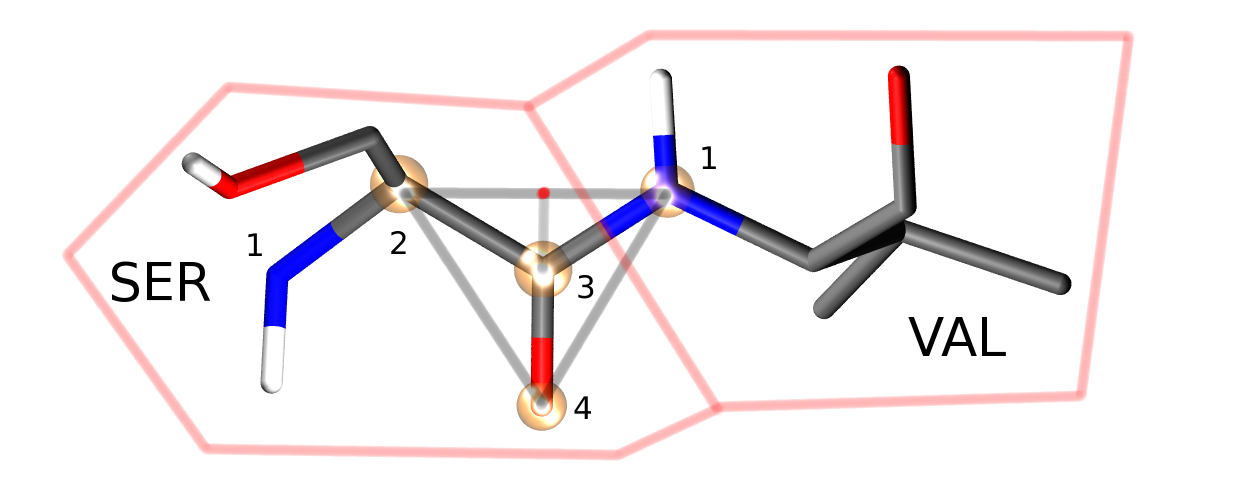
\includegraphics{backbone.png}}
\caption{Four atoms from each protein residue are designated as backbone atoms (bbatoms). For most residues these atoms are the N, CA, C and O atoms respectively. The four backbone atoms for two neighbouring residues are shown above. The protein backbone move moves the last three bbatoms of one residue and the first bbatom of the next residue. This is because the moves assumes that these four bbatoms form a rigid triangle (as is shown by the grey lines). The four atoms are translated and rotated as a rigid triangle, with the origin of rotation of the triangle centered on the intersection of the vector between bbatoms 2 and 1, and the vector between bbatoms 3 and 4 (marked as a red dot directly above the C=O bond). Because this triangle is translated and rotated as a rigid unit, all atoms connected to the atoms of this triangle will also be translated and rotated as a rigid unit.}\end{figure}

Four special backbone atoms (bbatoms) are identified in the chain-backbone of each residue. These atoms form the reference from which the rest of the residue atoms are built. These four atoms can be translated and rotated as a rigid unit via protein backbone moves (see figure above). As the rest of the residue is constructed from these bbatoms, the rest of the residue is thus also translated and rotated. Because the bbatoms are translated and rotated as a rigid unit, the internal geometry of these backbone atoms are held constant throughout the simulation. This means that the internal geometry of the bbatoms is taken from the PDB file, and may not be modified by the chain or residue templates. It is also not possible to build missing bbatoms, so they must all be present in the PDB file.

Once the coordinates and z-matrices of each residue have been assigned, interresidue bonds are added between the first bbatom of each residue and the third bbatom of the previous residue (e.g. for ‘ASP’, bonds would be added from the ‘N’ atom of the ‘ASP’ residue to the ‘C’ atom of the preceeding amino acid residue). If the length of this bond is less than 4 A then this bond is added as a real bond, and its energy is evaluated as part of the forcefield. However, if the length is greater than 4 A, then this bond will be added as a dummy bond, and a warning message output. This is useful in cases where you wish to load up a protein scoop, e.g. from around the active site. This option should be used with care in conjunction with backbone moves.


\begin{threeparttable}
\capstart\caption{Table 1.0 The default value of the maximum number of proteins, GCsolutes, solutes and solvents that may be loaded simultaneously by ProtoMS. These values may be changed by editing the dimensions.inc file located in the src directory, and recompiling ProtoMS.}

\begin{tabulary}{\linewidth}{|L|L|L|}
\hline
\textsf{\relax 
Parameter
} & \textsf{\relax 
Description
} & \textsf{\relax 
Values
}\\
\hline
MAXPROTEINS
 & 
Maximum number of proteins
 & 
3
\\
\hline
MAXRESIDUES
 & 
Maximum number of residues per protein
 & 
500
\\
\hline
MAXSCATOMS
 & 
Maximum number of atoms per protein residue
 & 
30
\\
\hline
MAXSOLUTES
 & 
Maximum number of solutes
 & 
25
\\
\hline
MAXSOLUTERESIDUES
 & 
Maximum number of residues per solute
 & 
25
\\
\hline
MAXSOLUTEATOMSPERRESIDUE
 & 
Maximum number of solute atoms per residue
 & 
50
\\
\hline
MAXSOLVENTS
 & 
Maximum number of solvent molecules
 & 
10000
\\
\hline
MAXSOLVENTS
 & 
Maximum number of GCsolute molecules
 & 
10000
\\
\hline
MAXSOLVENTATOMS
 & 
Maximum number of atoms per solvent
 & 
10
\\
\hline\end{tabulary}

\end{threeparttable}


\textbf{Limits}

ProtoMS is written using slightly extended Fortran 77 (see {\hyperref[compilation:fortran77]{\emph{Programming Language}}}). This means that the maximum numbers of loaded proteins, solutes and solvents has to be set at compile time. Table 1.0 gives the default values for the maximum number of proteins, solutes and solvents. Please note that you may change these numbers to fit the system that you are interested in, e.g. if you were investigating a single protein in a lipid bilayer then you may choose to model the lipid as a solute (thus requiring a large increase in the number of solute molecules, but a decrease in the number of solute residues), and you could reduce the maximum number of protein molecules to one. By balancing the numbers of protein, solutes and solvents you should find that you are able to load up the system that you want to simulate.

\index{Forcefields}

\section{Classical forcefields}
\label{protoms:index-5}\label{protoms:classical-forcefields}
ProtoMS was designed to perform simulations using a range of different molecular mechanics (MM) forcefields. To achieve this aim, a generic forcefield has been implemented, and this can be specialised into a specific, traditional forcefield.

The forcefield in ProtoMS is comprised of several terms;

\index{Intermolecular Potential}\index{Coulomb Potential}\index{van der Waals Potential}
\textbf{Intermolecular Potential}

An intermolecular potential acts between all molecules within the system. The intermolecular potential between a pair of molecules, \emph{A} and \emph{B}, \(U_{molecule} (A, B)\), with \emph{A} consisting of \(n_A\) atoms and \emph{B} consisting of \(n_B\) atoms, is formed as the sum of the non-bonded potential, \(U_{nb} (i, j)\) between each pair of atom sites, \emph{i} and \emph{j}, between the two molecules, scaled by a constant, \emph{scl}, e.g.
\phantomsection\label{protoms:equation-intermol1}\begin{gather}
\begin{split}U_{molecule}(A,B) = scl(R)\times\biggl( \sum_{i=1}^{n_A} \sum_{j=1}^{n_B} U_{nb}(i,j) \biggr)\end{split}\label{protoms-intermol1}
\end{gather}
where \emph{R} is the shortest distance between a pair of atom sites between the molecules. The scaling factor is set according to
\begin{gather}
\begin{split}&R \ge r_{cut} \rightarrow scl = 0.0 \\\end{split}\notag\\\begin{split}&r_{cut}-r_{feather} \le R \le r_{cut} \rightarrow scl = \frac{r_{cut}^2-R^2}{r_{cut}^2-(r_{cut}-r_{feather})^2} \\\end{split}\notag\\\begin{split}&R \le r_{feather} \rightarrow scl = 1.0,\end{split}\notag
\end{gather}
where \(r_{cut}\) and \(r_{feather}\) are the non-bonded cutoff and feather parameters.

The non-bonded potential between the pair of atoms is evaluated as the sum of the Coulombic and Lennard-Jones (LJ) potentials between the atoms,
\phantomsection\label{protoms:equation-intermol2}\begin{gather}
\begin{split}U_{nb}(i,j) = \frac{q_i q_j}{4\pi\epsilon_{0} r(i,j)} + 4\epsilon_{ij}\biggl[ \biggl(\frac{\sigma_{ij}}{r(i,j)}\biggr)^{12} - \biggl(\frac{\sigma_{ij}}{r(i,j)}\biggr)^6 \biggr],\end{split}\label{protoms-intermol2}
\end{gather}
where \(q_i\) and \(q_j\) are the partial charges on the two atom sites, \emph{r(i, j)} is the distance between the atom sites, \(\epsilon_0\) is the permittivity of free space and \(\sigma_{ij}\) and \(\epsilon_{ij}\) are the Lennard Jones parameters for the atom site pair \emph{i} and \emph{j}. The LJ parameters for an atom site pair are calculated as the average of the LJ parameters for the same site pair.

\index{combination rules}
Either the arithmetic average is used, or the geometric average is used, e.g.
\phantomsection\label{protoms:equation-arithmetriccomb}\begin{gather}
\begin{split}\sigma_{ij} = 0.5\times(\sigma_{ii} + \sigma_{jj}).\end{split}\label{protoms-arithmetriccomb}
\end{gather}\phantomsection\label{protoms:equation-geometriccomb}\begin{gather}
\begin{split}\epsilon_{ij} = \sqrt{\epsilon_{ii}\times\epsilon_{jj}}.\end{split}\label{protoms-geometriccomb}
\end{gather}
The AMBER family of forcefields use the arithmetic average for \(\sigma\), and the geometric average for \(\epsilon\), while the OPLS family of forcefields use the geometric average for both parameters. The intermolecular potential is formed as the sum of the non-bonded potential over all pairs of atom sites. It should be noted that an atom site does not necessarily need to lie at the center of each atom, and it may lie between atoms, or at the location of any lone pairs. Individual atoms may possess many atom sites, or even no atom sites.

\index{Bond Potential}
\textbf{Bond Potential}

A bond potential acts over all of the explicitly added, non-dummy bonds within a molecule. ProtoMS makes no attempt to find any implicit bonds within a molecule, and it is not possible to add a bond between atoms of different molecules. The energy of each bond, \(U_{bond}\) , is evaluated according to
\phantomsection\label{protoms:equation-bondpot}\begin{gather}
\begin{split}U_{bond}(r) = k_{bond}\bigl(r-r_0\bigr)^2,\end{split}\label{protoms-bondpot}
\end{gather}
where \emph{r} is the bond length, \(k_{bond}\) is the force constant for the bond, and \(r_0\) is the equilibrium bond length. The total bond energy of a molecule is the sum of the bond energies for all of the bonds within the molecule, and the total bond energy of the system is the sum of the bond energies for each of the molecules in the system.

\index{Angle Potential}
\textbf{Angle Potential}

An angle potential acts over all angles between atoms that are connected by non-dummy bonds, and over all
non-dummy angles that have been explicitly added to the molecule. The energy of each angle, Uangle , is evaluated
according to
\phantomsection\label{protoms:equation-angpot}\begin{gather}
\begin{split}U_{angle}(\theta) = k_{angle}\bigl(\theta-\theta_0\bigr)^2,\end{split}\label{protoms-angpot}
\end{gather}
where \(\theta\) is the size of the angle, \(k_{angle}\) is the force constant for the angle, and \(\theta_0\) is the equilibrium angle size. The total angle energy of a molecule is the sum of the angle energies for each of the angles within the molecule, and the total energy of the system is the sum of the angle energies for each of the molecules in the system.

\index{Urey-Bradley Potential}
\textbf{Urey-Bradley Potential}

A Urey-Bradley potential may act between the first and third atoms of some of the angles that are evaluated for the angle potential. If this is the case, then a Urey-Bradley energy is added onto the angle energy. The Urey-Bradley energy, \(U_{uby}\), is evaluated according to
\phantomsection\label{protoms:equation-ubpot}\begin{gather}
\begin{split}U_{uby}(x) = k_{uby}\bigl(x-x_0\bigr)^2,\end{split}\label{protoms-ubpot}
\end{gather}
where \emph{x} is the distance between the first and third atoms, \(k_{uby}\) is the Urey-Bradley force constant, and \(x_0\) is the equilibrium distance.

\index{Dihedral Potential}
\textbf{Dihedral Potential}

A dihedral potential acts over all dihedrals between atoms that are connected by non-dummy bonds, and over all non-dummy dihedrals that have been explicitly added to the molecule. Such explicitly added dihedrals may be used to add improper dihedrals that maintain the stereochemistry of chiral centers. The energy for each dihedral, \(U_{dihedral}\), is formed as the sum of \emph{n} cosine terms,
\phantomsection\label{protoms:equation-dihepot}\begin{gather}
\begin{split}U_{dihedral}(\phi) = \sum_{i=1}^{n} k_{i1}\bigl[1.0 + k_{i2}\bigl(cos(k_{i3}\phi + k_{i4})\bigr)\bigr],\end{split}\label{protoms-dihepot}
\end{gather}
where \(k_{i1}\) to \(k_{i4}\) are dihedral parameters and \(\phi\) is the size of the dihedral. The total dihedral energy of a molecule is the sum of the dihedral energies for each of the dihedrals in the molecule, and the total dihedral energy of the system is the sum of the dihedral energies of each of the molecules.

\index{Intramolecular non-bonded Potential}
\textbf{Intramolecular non-bonded Potential}

An intramolecular non-bonded potential acts between all intramolecular pairs of atoms that are either not connected by a non-dummy bond, or are not both connected to a third atom by a non-dummy bond. To make this more clear, if two atoms are connected by a non-dummy bond then they are said to be 1-2 bonded. If two atoms are both connected to a third atom by non-dummy bonds, then they are said to 1-?-3, or 1-3 bonded. Similarly, if the pair of atoms are connected together via two atoms via non-dummy bonds, then they are said to be 1-?-?-4, or 1-4 bonded. An intramolecular non-bonded potential does not act over 1-2 or 1-3 bonded pairs within a molecule, but does act over 1-4 bonded pairs and above. Note that ProtoMS only looks at the non-dummy bonds between atoms, and will not consider whether or not there are non-dummy angles, Urey-Bradley or dihedral terms involving these atoms.

The intramolecular non-bonded potential of a molecule, \(U_{intra}\) is the sum of the non-bonded energy between all 1-5 and above pairs of atoms within the molecule, plus the sum of the non-bonded energy between all 1-4 atoms scaled by a 1-4 scaling factor, e.g.
\phantomsection\label{protoms:equation-intrapot1}\begin{gather}
\begin{split}U_{intra} = &\sum_{\text{1-5+ i j pairs}} U_{coul}(i,j) + U_{lj}(i,j) + \sum_{\text{1-4 i j pairs}} scl_{coul} U_{coul}(i,j) + scl_{lj} U_{lj}(i,j),\end{split}\label{protoms-intrapot1}
\end{gather}
where
\phantomsection\label{protoms:equation-intrapot2}\begin{gather}
\begin{split}U_{coul}(i,j) = \frac{q_i q_j}{4\pi\epsilon_{0} r},\end{split}\label{protoms-intrapot2}
\end{gather}
and
\phantomsection\label{protoms:equation-intrapot3}\begin{gather}
\begin{split}U_{lj}(i,j) = 4\epsilon_{ij}\biggl[ \biggl(\frac{\sigma_{ij}}{r}\biggr)^{12} - \biggl(\frac{\sigma_{ij}}{r}\biggr)^6 \biggr].\end{split}\label{protoms-intrapot3}
\end{gather}
Equations \eqref{protoms-intrapot2} and \eqref{protoms-intrapot3} are the Coulomb and Lennard Jones equations, as seen in the intermolecular potential in equations \eqref{protoms-intermol1} and \eqref{protoms-intermol2}. \(scl_{coul}\) and \(scl_{lj}\) are the Coulomb and Lennard Jones scaling factors.

\index{GBSA Potential}
\textbf{Generalized Born Surface Area potential}

While free energy simulations are usually conducted in explicit solvent, ProtoMS supports Generalized Born Surface Area (GBSA) implicit solvent models. Relatively few free energy implicit solvent studies have been conducted and such option should be tested carefully before embarking onto expensive free energy simulations. The GBSA theory assumes that the total solvation free energy of a molecule A is a sum of a polar and non-polar energy term:
\phantomsection\label{protoms:equation-gb1}\begin{gather}
\begin{split}\Delta G_{solv} = \Delta G_{pol} + \Delta G_{nonpol}\end{split}\label{protoms-gb1}
\end{gather}
The second term, is simply proportional to the solvent accessible surface area (SASA) of the molecule, times a parameter that depends on the atom types present in the molecule. The first term is more complex and derived from the following equation :
\phantomsection\label{protoms:equation-gb2}\begin{gather}
\begin{split}\Delta G_{pol} = -\frac{1}{2}(\frac{1}{\epsilon_{vac}}-\frac{1}{\epsilon_{solv}})  \sum_{i}\sum_{j} \frac{q_{i}q_{j}}{\sqrt{r^{2}_{ij} + B_{i}B_{j} e^{\frac{-r^{2}_{ij}}{4B_{i}B_{j}}}   } }\end{split}\label{protoms-gb2}
\end{gather}
\(\epsilon_{vac}\) and \(\epsilon_{solv}\) are the dielectric constants of the vacuum and the solvent respectively, \(q_{i}\) the atomic partial charge of atom \emph{i}, \(r_{ij}\) the distance between a pair of atoms \emph{ij}, and \(B_{i}\) is the effective Born radius of atom \emph{i}.

The effective Born Radius \(B_{i}\) is in essence the spherically averaged distance of the solute atom to the solvent. An accurate estimate of this quantity is essential to calculate high quality solvation free energies. It is however fairly complex to compute as it formalyl involves an integral over the position of all the atoms in the system. While numerical techniques can calculate such value, they are too slow to be of practical use in a simulation. In ProtoMS, the effective Born radii are calculated using the Pairwise Descreening Approximation (PDA) method.
\begin{gather}
\begin{split}{\frac{1}{B_i}} = \frac{1}{\alpha _{i}} - \frac{1}{2} \sum_{j \not= i} \lbrack \frac{1}{L_{ij}}-\frac{1}{U_{ij}}+\frac{r_{ij}}{4}(\frac{1}{U_{ij}^{2}}-\frac{1}{L_{ij}^{2}}) +\frac{1}{2r_{ij}}ln\frac{L_{ij}}{U_{ij}} + \frac{S_{j}^{2}\alpha_{j}^{2}}{4r_{ij}}(\frac{1}{L_{ij}^{2}}-\frac{1}{U_{ij}^{2}} ) \rbrack\end{split}\notag\\\begin{split}L_{ij} &= 1 \quad if \quad r_{ij} + S_{j}\alpha_{j} \leq \alpha_{i} \\\end{split}\notag\\\begin{split}L_{ij} &= \alpha_{i} \quad if \quad r_{ij} - S_{j}\alpha_{j} \leq \alpha_{i}  <r_{ij} + S_{j}\alpha_{j}\\\end{split}\notag\\\begin{split}L_{ij} &= r_{ij} - S_{j}\alpha_{j} \quad if \quad \alpha_{i} \leq r_{ij} - S_{j}\alpha_{j}\\\end{split}\notag\\\begin{split}U_{ij} &= 1 \quad if \quad  r_{ij} + S_{j}\alpha_{j} \leq \alpha_{j}\\\end{split}\notag\\\begin{split}U_{ij} &= r_{ij} + S_{j}\alpha_{j} \quad if \quad \alpha{i} <  r_{ij} + S_{j}\alpha_{j}\\\end{split}\notag
\end{gather}
where \(r_{ij}\) is the distance between a pair of atoms \emph{ij} and \(\alpha_{i}\) is the intrinsic Born radius of atom \emph{i}, that is, the Born radius that atom \emph{i} would adopt if it was completely isolated. Finally \(S_{j}\) is a scaling factor which compensates for systematic errors introduced by this approximate Born radii calculation.

As the name says, the technique approximate the descreening (the extent to which a nearby atom j displaces a volume that would have otherwise been occupied by solvent) by a fast summation of pairwise terms. It is however not rigorous and has to be parameterised carefully to yield robust performance. The PDA method tend to systematically underestimate the Born radius of buried atoms because it incorrectly assign high dielectric constants to numerous small voids and crevices that exist between atoms in a protein and are not occupied by water. To increase accuracy, a re-scaling technique has been implemented.
\begin{gather}
\begin{split}{\frac{1}{B_i}}  = \frac{1}{\alpha _{i}} - Itanh\big( \alpha \psi - \beta \psi^{2} + \gamma \psi^{3}  \big)\end{split}\notag
\end{gather}
where \emph{I} is the summation term from the PDA calculation, \(\psi\), \(\alpha\), \(\beta\) and \(\gamma\) are parameters taken from the litterature.

The rescaling option has not been used extensively in ProtoMS and should be used with caution. It appears it may prove useful when simulation buried protein binding sites.

The GBSA force field implemented in ProtoMS was parameterised to be used with the AMBER99 and the GAFF force fields. While alternative force fields could be used, a loss of accuracy could be expected.

GBSA simulations are order of magnitude more efficient than explicit solvent simulations of small isolated molecules. However, they slow
down rapidly when the size of the system increases. This is especially notable in Monte Carlo simulations where a small movement of part of a system formally warrants the computation the entire solvation energy of the system. This issue arises because the GBSA energy terms are not strictly pairwise decomposable.  It is possible to use however different techniques to increase the speed of a GBSA simulation. Cutoffs in the calculation of the Born radii are introduced and in addition the update of pairwise GB energies can be skipped if the Born radii of either atoms have not changed more than a certain threshold value after a MC move. Because this option will introduce energy drifts, it is advised to periodically recalculate rigorously the GB energy. In addition, a more complex Monte Carlo move is implemented in ProtoMS. This option allows to conduct a simulation with a crude GBSA model and a low cutoff for the non bonded energy terms. Normally the  predicted macroscopic properties would suffer from such crude treatment of intermolecular energies. However, periodically, a special acceptance test is employed to remove the bias introduced by the crude potential and ensure that the equilibrium density of states generated by the Monte Carlo simulation converges to the equilibrium density of states suitable for the standard biomolecular potential.

Actual speedups using either techniques are system dependent and optimisation of the different parameters can be a complex task. It is advised to use the default parameters described latter in the manual.

\textbf{Caveats}

ProtoMS implements this forcefield mostly as described. However there are a few shortcuts that are taken to improve the efficiency of the code. These shortcuts are based on the three-way split of the molecules of the system into solvents, solutes and proteins
\begin{itemize}
\item {} 
\textbf{solvents} As solvents are rigid, there is no need to evaluate any of the intramolecular potentials. ProtoMS thus only evaluates the intermolecular energy of solvent molecules.

\item {} 
\textbf{solutes} ProtoMS evaluates the forcefield of solute molecules exactly as described, with no shortcuts. proteins ProtoMS implements a protein as a chain of residues. As these molecules can be large, and typically larger than the non-bonded cutoff, ProtoMS implements the non-bonded cutoff differently for

\item {} 
\textbf{proteins}. Instead of evaluating the non-bonded cutoff for the protein as a whole, ProtoMS implements a residue-based cutoff, with the cutoff scaling factors evaluated individually for each residue. Additionally, the intramolecular non-bonded energy is also scaled according to the non-bonded cutoffs given in equation \eqref{protoms-intermol1}. If you do not want to use residue based cutoffs, then it is possible to tell ProtoMS to use a molecule based cutoff, in which case the forcefield for proteins will be evaluated exactly as described with no shortcuts.

\end{itemize}

\index{Perturbations}

\section{Perturbations}
\label{protoms:index-14}\label{protoms:perturbations}
ProtoMS is capable of calculating the relative free energy of two systems. ProtoMS does this by perturbing one system into the other through the use of a \(\lambda\)-coordinate. If A and B are the two systems of interest, then the forcefield is constructed such that at \(\lambda\) = 0.0 the forcefield represents system A, at \(\lambda\) = 1.0 the forcefield represents system B, and at \(\lambda\) value inbetween, the forcefield represents a hybrid of A and B.

ProtoMS implements two methods of perturbing between systems A and B;
\begin{itemize}
\item {} 
\textbf{Single topology} System A is perturbed into system B by scaling the forcefield parameters such that the model morphs from A to B.

\item {} 
\textbf{Dual topology} System A and B are simulated together, with \(\lambda\) scaling the total energies of A and B such that one system is turned off as the other is turned on.

\end{itemize}

\index{Single Topology}
\textbf{Single Topology Calculations}

ProtoMS assigns two sets of parameters to every single forcefield term; one parameter represents that term at \(\lambda=0.0\) (\(par_0\)), the other represents that term at \(\lambda=1.0\) (\(par_1\)). \(\lambda\) is used to linearly scale between these two parameters to obtain the value of the parameter at each value of \(\lambda\) (\(par_\lambda\))
\phantomsection\label{protoms:equation-lambdamix}\begin{gather}
\begin{split}par_\lambda = (1.0-\lambda) \times par_0 + \lambda \times par_1.\end{split}\label{protoms-lambdamix}
\end{gather}
This equation is used to scale the charge, \(\sigma\) and \(\epsilon\) parameters assigned to each atom site (see equations \eqref{protoms-intermol1}), and the force constants (\(k_{bond}\), \(k_{angle}\) and \(k_{uby}\)) and equilibrium sizes (\(r_0\), \(\theta_0\) and \(x_0\)) for the bond, angle and Urey-Bradley terms (see equations \eqref{protoms-bondpot}, \eqref{protoms-angpot} and \eqref{protoms-ubpot}). This equation is not used to scale the dihedral parameters, as the functional form of the dihedral potential is more complicated. Rather than scale the dihedral parameters, ProtoMS uses \(\lambda\) to scale the total energy of each dihedral;
\phantomsection\label{protoms:equation-dihmix}\begin{gather}
\begin{split}U_{dihedral}(\phi)_\lambda = (1.0-\lambda)\times U_{dihedral}(\phi)_0 + \lambda \times U_{dihedral}(\phi)_1,\end{split}\label{protoms-dihmix}
\end{gather}
where \(U_{dihedral}(\phi)_0\) is the dihedral energy using the parameters for \(\lambda=0.0\), \(U_{dihedral}(\phi)_1\) is the dihedral energy using the parameters for \(\lambda=1.0\), and \(U_{dihedral}(\phi)_\lambda\) is the scaled dihedral energy at that value of \(\lambda\).

Any and all parts of the forcefield can be scaled. This includes all of the forcefield parameters of any solutes, all of the parameters of any proteins, and all parameters of any solvent molecules. While this is very useful, and enables perturbations of any and all parts of the system, there are many cases where just changing the forcefield parameters is not sufficient to smoothly morph from one system into the other. There are many cases where the geometry of the molecules needs to be changed with \(\lambda\). Fortunately ProtoMS provides this capability for solute molecules. Any internal coordinates that are part of the z-matrix of a solute molecule may perturbed with \(\lambda\). Geometry variations are a powerful tool as they allow for very complicated, yet very smooth transitions between two systems to be described. A good example of such a transition is the annihilation of the hydrogen atoms as a methyl group is morphed into a single hydrogen.
\begin{figure}[htbp]
\centering
\capstart

\scalebox{0.500000}{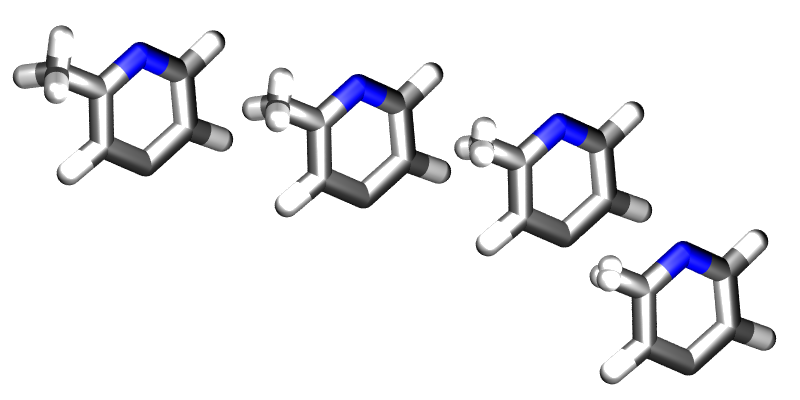
\includegraphics{alchemy.png}}
\caption{Geometry variations allow for a smoother transition between two systems, for example here a methyl group is smoothly converted into a hydrogen.}\end{figure}

As well as enabling smooth transitions between systems, geometry variations may be used to calculate potentials of mean force along structural coordinates.

\index{Dual Topology}
\textbf{Dual Topology Calculations}

A dual topology method to calculate free energy changes is also available in ProtoMS. In the single topology method force field terms were linearly interpolated so that they match the force field parameters suitable for particular molecule at either end of the perturbation (\(\lambda\) 0.0 or \(\lambda\) 1.0). As two molecules often differ not only in their force field terms but also their geometry, it is often necessary to modify the internal coordinates as well. This is relatively easy In simple cases (morphing a methyl group into a hydrogen group) but for larger, complex, perturbations this is often cumbersome if not impossible. In the dual topology method no geometry variations are attempted. However, the interaction energy of a pair of solutes with their surroundings (solvent, protein, other solutes), is gradually turned on or off with the coupling parameter.
\phantomsection\label{protoms:equation-doubletopu}\begin{gather}
\begin{split}U(\lambda) = U_{0} + \lambda U(S_{2}) + (1 - \lambda) U(S_{1})\end{split}\label{protoms-doubletopu}
\end{gather}
Equation \eqref{protoms-doubletopu} thus shows that at any given value of \(\lambda\), the total energy of the system consists in a term \(U_{0}\) that is independent of the perturbation and a term \(U(S_{2})\) and \(U(S_{1})\) which is a function of the intermolecular energies of the pair of solutes for which a free energy change is to be calculated.

A dual topology setup is simpler and more generally applicable than a single topology setup. However dual topology approaches suffer from a number of technical difficulties which are mainly related to the fact that if a solute does not have any intermolecular interaction with its surroundings, it can drift anywhere in the simulation box. This usually causes the free energy difference to converge very very slowly (in practice not at all). To overcome these difficulties, the dual topology technique implemented in ProtoMS constrains a pair of solutes to stay together by the introduction of dummy bond between the center of geometry of the two solutes. As this does not prove to be sufficient to avoid convergence issues, a soft-core non bonded energy function is also implemented. In essence, the function that computes the intermolecular energy of the solutes is modified such that when a solute is not fully interacting with its surroundings, it's Lennard-Jones and couloumbic energies are softened such that atomic overlaps do not result in very large, positive, energies. The solute is effectively `softer'. There are three soft-core versions implemented in ProtoMS. The original implementation in ProtoMS for a solute
that is being turned off is described by equation \eqref{protoms-uljsoftmod}.
\phantomsection\label{protoms:equation-uljsoftmod}\begin{gather}
\begin{split}U_{non bonded,\lambda}= (1-\lambda) 4{\epsilon}_{ij} \left[ \left( \frac{ \sigma_{ij}^{12} }{ ( \lambda \delta \sigma_{ij} + r_{ij}^{2} )^{6}} \right) - \left( \frac{ \sigma_{ij}^{6} }{ (\lambda \delta \sigma_{iJ}  + r_{ij}^{2})^{3} } \right) \right] +  \frac{(1-\lambda)^{n} q_{i}q_{j}} {4\pi{\epsilon}_{0}\sqrt{(\lambda +  r_{ij}^{2})}}\end{split}\label{protoms-uljsoftmod}
\end{gather}
where the parameters n and \(\delta\) control the softness of the Coulombic and Lennard-Jones interactions respectively.

An alternative that has been useful in some applications is described by equation \eqref{protoms-uljsoftmod2}
\phantomsection\label{protoms:equation-uljsoftmod2}\begin{gather}
\begin{split}U_{non bonded,\lambda}= (1-\lambda) 4{\epsilon}_{ij} \left[  \left( \frac{ \sigma_{ij}^{12} }{ ( \lambda \delta \sigma_{ij}^6 + r_{ij}^{6} )^{2}} \right) -  \left( \frac{ \sigma_{ij}^{6} }{ \lambda \delta \sigma_{iJ}^6  + r_{ij}^{6} } \right) \right] +  \frac{(1-\lambda)^{n} q_{i}q_{j}} {4\pi{\epsilon}_{0} \left [ \lambda \delta_c +  r_{ij}^{6} \right ]^{1/6}}\end{split}\label{protoms-uljsoftmod2}
\end{gather}
with an additional softness parameter \(\delta_c\) for the Coulombic interactions.

Third, the soft-core implementation in the latest version of the Amber package is available and is described by equation \eqref{protoms-uljsoftmod3}
\phantomsection\label{protoms:equation-uljsoftmod3}\begin{gather}
\begin{split}U_{non bonded,\lambda}= (1-\lambda) 4{\epsilon}_{ij} \left[ \left( \frac{ \sigma_{ij}^{12} }{ ( \lambda \delta \sigma_{ij}^6 + r_{ij}^{6} )^{2}} \right) - \left( \frac{ \sigma_{ij}^{6} }{ \lambda \delta \sigma_{iJ}^6 + r_{ij}^{6} } \right) \right] +  \frac{(1-\lambda)^{n} q_{i}q_{j}} {4\pi{\epsilon}_{0} \sqrt{( \lambda \delta_c +  r_{ij}^{2})}}\end{split}\label{protoms-uljsoftmod3}
\end{gather}

\section{Generic Moves}
\label{protoms:generic-moves}\label{protoms:moves}
ProtoMS conducts a simulation by performing a sequence of moves on the system. The following moves are currently implemented
\begin{itemize}
\item {} 
\textbf{Residue moves} Standard Monte Carlo (MC) moves on protein residues.

\item {} 
\textbf{Solute moves} Standard MC moves on solute molecules.

\item {} 
\textbf{Solvent moves} Standard MC moves on solvent molecule.

\item {} 
\textbf{Volume moves} Monte Carlo moves that change the volume of the system. These are used to run constant pressure simulations.

\item {} 
\textbf{GCSolute moves} Standard MC moves on GCsolute molecules.

\item {} 
\textbf{Insertion moves} MC moves which selects a GCsolute with a \(\theta\) value of 0 and turns it to 1

\item {} 
\textbf{Deletion moves} MC moves which selects a GCsolute with a \(\theta\) value of 1 and turns it to 0

\item {} 
\textbf{Theta moves} MC moves which sample the value of \(\theta\) on a GCsolute molecule

\item {} 
\textbf{Sample moves} MC moves which sample the value of \(\theta\) on a GCsolute molecule whilst applying a biasing potential \(\lambda\)-moves Monte Carlo moves that change \(\lambda\). These may be used to perform umbrella sampling free energy simulations.

\item {} 
\textbf{Dual potential moves} Works only with implicit solvent simulations. Allows to sample rapidly configurations with a crude potential but correct for errors with a specific acceptance test.

\end{itemize}

\index{Residue Moves}
\textbf{Residue Moves}
A residue move is a Monte Carlo move on a single protein residue. Obviously, for a residue move to be be performed, at least one protein that has flexible residues must be loaded. Each residue move comprises the following steps
\begin{enumerate}
\item {} 
A protein is picked randomly from the set of proteins that have flexible residues. Note that each protein is weighted equally, so each protein has an equal chance of being chosen, regardless of how many flexible residues it contains. This behaviour is likely to change in future versions of the code, as ideally the probability of choosing to move a protein should be proportional to the number of flexible residues.

\item {} 
One of the flexible residues within the protein is chosen randomly from the set of all flexible residues in the protein. Again, there is no weighting of residues, so each flexible residue has an even chance of being chosen, despite the size of each residue.

\item {} 
If the backbone of this residue is flexible, then a random number between 1 and 3 is generated. If the random number is equal to 1, then only a backbone move on the residue will be attempted. If the random number is equal to 2 then only a sidechain move will be attempted, where all of the flexible internals of the residue are moved. If the random number is equal to 3 then a backbone and sidechain move are attempted simultaneously. If the backbone of this residue is fixed, then only a sidechain move is attempted.

\item {} 
The change in energy that results from this move is evaluated, and then tested according to the Metropolis criterion to decide whether or not to accept the move.

\item {} 
If the move is accepted, then the new configuration of the residue is saved. If the move was rejected then the original configuration of the residue is restored.

\end{enumerate}

You can change the flexibility of any residue in any protein by using the fixbackbone and fixresidues commands described in section {\hyperref[protoms:misccmd]{\emph{Miscellaneous}}}. All residues of all proteins are flexible by default, and have flexible backbones. Note that the backbone move is still experimental and not thouroughly tested. I recommend that you fix the backbone of all residues for production simulations. You control the maximum amounts that the residue moves via the residue template (see {\hyperref[protoms:temref]{\emph{Templates}}}). The actual amount that a residue moves by will be based on random values generated within the limits of the maximum amounts set in the residue template, e.g. if the maximum change of an angle was \(5.0^\circ\) , then the angle will be changed by a random value generated evenly between \(-5.0^\circ\) and \(+5.0^\circ\).

\index{Solute Moves}
\textbf{Solute Moves}
A solute move is a Monte Carlo move on a single solute molecule. Obviously, for a solute move to be performed, at least one solute molecule must be loaded. Each solute move comprises the following steps
\begin{enumerate}
\item {} 
A solute is picked randomly from the set of loaded solutes. Each solute is weighted equally, regardless of its size or numbers of degrees of freedom.

\item {} 
One of the residues is chosen at random within the solute. Again, each residue is weighted equally, regard- less of its size.

\item {} 
All of the flexible internals of this residue are changed, and the whole solute molecule is randomly translated, and rotated around its center of geometry.

\item {} 
The change in energy associated with this move is evaluated and then tested via the Metropolis criterion to decide whether or not to accept the move.

\item {} 
If the move is accepted then the new configuration of the solute is saved. If the move was rejected then the original configuration is restored. You can control the maximum amounts that the solute moves via the solute template (see {\hyperref[protoms:temref]{\emph{Templates}}}).

\end{enumerate}

\index{Solvent Moves}
\textbf{Solvent Moves}

A solvent move is a Monte Carlo move on a single solvent molecule. Obviously, for a solvent move to be performed, at least one solvent molecule must be loaded. Each solvent move comprises the following steps
\begin{enumerate}
\item {} 
A solvent molecule is randomly chosed from the set of loaded solvent molecules. If preferential sampling is turned on (see {\hyperref[protoms:parameters]{\emph{Simulation parameters}}}), then the solvent molecules closest to the preferred solute have a relatively higher weight, so will be more likely to be chosen. If preferential sampling is off, then each solvent is weighted equally, regardless of its relative size or proximity to a solute.

\item {} 
The solvent molecule is randomly translated and rotated around its center of geometry.

\item {} 
The change in energy associated with this move is evaluated and used to decide whether or not to accept this move via the Metropolis criterion if preferential sampling was turned off, or via a biased Monte Carlo test if preferential sampling were turned on.

\item {} 
If the move was accepted then the new solvent configuration is saved, otherwise the original configuration is restored.

\end{enumerate}

You can control the maximum amounts that the solvent is translated and rotated by by editing its solvent template (see {\hyperref[protoms:temref]{\emph{Templates}}}).

\index{Volume Moves}
\textbf{Volume Moves}

A volume move is a Monte Carlo move that changes the volume of the system. This is needed to be able to perform Monte Carlo simulations at constant pressure (i.e. using the NPT ensemble). For a volume move to be performed you need to have loaded a box of solvent molecules, and be running using periodic boundary conditions. A volume move is comprised of the following steps
\begin{enumerate}
\item {} 
A random change in volume is chosen within the range set via the maxvolchange command (see {\hyperref[protoms:parameters]{\emph{Simulation parameters}}}).

\item {} 
The volume of the system is changed by this amount by scaling all of the coordinates evenly from the center of the simulation box.

\item {} 
The change in energy associated with this change in volume is evaluated and used to decide whether or not to accept this move via the constant pressure Monte Carlo test, for the system pressure set via the pressure command (see {\hyperref[protoms:parameters]{\emph{Simulation parameters}}}).

\item {} 
If the move is accepted then the new system configuration is saved, otherwise the original system configuration is restored.

\end{enumerate}

\index{GCSolute Moves}
\textbf{GCsolute Moves}

A GCsolute move is a Monte Carlo move on a single Gcsolute molecule. Each GCsolute move comprises the following steps
\begin{enumerate}
\item {} 
A GCsolute molecule is randomly chosed from the set of loaded GCsolute molecules.

\item {} 
The GCsolute molecule is randomly translated and rotated around its center of geometry. If it attempts to leave the confines of its predefined cubic region then it experiences a huge energetic penalty, ensuring that the Metropolis move is rejected.

\item {} 
The change in energy associated with this move is evaluated and used to decide whether or not to accept this move via the Metropolis criterion.

\item {} 
If the move was accepted then the new GCsolute configuration is saved, otherwise the original configuration is restored.

\end{enumerate}

You can control the maximum amounts that the GCsolute is translated and rotated by by editing its template (see {\hyperref[protoms:temref]{\emph{Templates}}}).

\index{Insertion Moves}
\textbf{Insertion Moves}

An insertion move is a Monte Carlo move on a single GCsolute molecule, whereby the \(\theta\) value of a GCsolute is turned from 0 to 1. Each insertion move comprises the following steps;
\begin{enumerate}
\item {} 
A GCsolute molecule is randomly chosed from the set of loaded GCsolute molecules. The value of \(\theta\) is examined; if it is set to 1 then another is chosen until the examined \(\theta\) value is 0

\item {} 
The value of \(\theta\) for that GCsolute molecule is set to 1, and the new energy associated with this value of \(\theta\) is calculated

\item {} 
The change in energy associated with this move is evaluated and used to decide whether or not to accept this move via the Metropolis criterion.

\item {} 
If the move was accepted then the new value of \(\theta\) for that GCsolute molecule is saved, otherwise the original value of 0 is restored.

\end{enumerate}

\index{Deletion Moves}
\textbf{Deletion Moves}

A deletion move is a Monte Carlo move on a single GCsolute molecule, whereby the \(\theta\) value of a GCsolute is turned from 1 to 0. Each deletion move comprises the following steps
\begin{enumerate}
\item {} 
A GCsolute molecule is randomly chosed from the set of loaded GCsolute molecules. The value of \(\theta\) is examined; if it is set to 0 then another is chosen until the examined \(\theta\) value is 1

\item {} 
The value of \(\theta\) for that GCsolute molecule is set to 0, and the new energy associated with this value of \(\theta\) is calculated

\item {} 
The change in energy associated with this move is evaluated and used to decide whether or not to accept this move via the Metropolis criterion.

\item {} 
If the move was accepted then the new value of \(\theta\) for that GCsolute molecule is saved, otherwise the original value of 1 is restored.

\end{enumerate}

\index{Theta Moves}
\textbf{Theta Moves}

A theta move is a Monte Carlo move on a single GCsolute molecule, whereby the \(\theta\) value of a GCsolute is sampled. Each theta move comprises the following steps
\begin{enumerate}
\item {} 
A GCsolute molecule is randomly chosed from the set of loaded GCsolute molecules

\item {} 
The value of \(\theta\) for that GCsolute molecule is randomly changed, and the new energy associated with this value of \(\theta\) is calculated

\item {} 
The change in energy associated with this move is evaluated and used to decide whether or not to accept this move via the Metropolis criterion.

\item {} 
If the move was accepted then the new value of \(\theta\) for that GCsolute molecule is saved, otherwise the original value of \(\theta\) is restored.

\end{enumerate}

\index{Sample Moves}
\textbf{Sample Moves}

A sample move is a Monte Carlo move on a single GCsolute molecule, whereby the \(\theta\) value of a GCsolute is sampled whilst applying a biasing potential, jbias. Each sample move comprises the following steps
\begin{enumerate}
\item {} 
A GCsolute molecule is randomly chosed from the set of loaded GCsolute molecules (typically only one GCsolute molecule is studied in a sample move)

\item {} 
The biasing potential is added onto the value of ieold for that molecule, based upon the volume of the restraint and the applied jbias

\item {} 
The value of \(\theta\) for that GCsolute molecule is randomly changed, and the new energy associated with this value of \(\theta\) is found

\item {} 
The biasing potential is added onto the value of ienew for that molecule, based upon the volume of the restraint and the applied jbias

\item {} 
The change in energy associated with this move is evaluated and used to decide whether or not to accept this move via the Metropolis criterion.

\item {} 
If the move was accepted then the new value of \(\theta\) for that GCsolute molecule is saved, otherwise the original value of \(\theta\) is restored.

\end{enumerate}

\index{Move Probabilities}
\textbf{Relative Move Probabilities}

You can specify which moves should be run by passing arguments to the simulate and equilibrate commands (see {\hyperref[protoms:runcmd]{\emph{Running a Simulation}}}). You can use these commands to assign a weight to each type of move, e.g. 100 for solvent moves, 10 for protein moves, 1 for solute moves and 0 for volume move. The type of move chosen for each step of the simulation is generated randomly based on these set relative weights. These weights mean that on average, in 111 moves, 100 of these moves will be solvent moves, 10 of these moves will be protein moves, 1 of these moves will be solute moves and none of the moves will be volume moves (e.g. no volume moves will be performed). Note that you need to perform some volume moves if you wish to sample from the NPT ensemble!


\chapter{Executing ProtoMS}
\label{protoms:executing-protoms}
ProtoMS is a simple program that may be used from the command line. Once you have compiled it you should find it in the top directory (it is called simply protoms3). If you run the program you should see that it prints out some information about the program and license, then it complains that nothing has been loaded so it closes down. The interface to ProtoMS has been designed to allow easy integration of ProtoMS with scripts, and to enable simple use from a command file. A ProtoMS input consists of a set of commands and values, e.g. the command \code{temperature} could have the value \emph{25.0} . This would set the simulation temperature to \(25^\circ\) C. The input is passed to ProtoMS via a command file. The above command could thus be input by setting by placing the line

\begin{Verbatim}[frame=single,commandchars=\\\{\}]
temperature 25.0
\end{Verbatim}

into a file and have ProtoMS read commands from that file. You specify the command file by passing it to ProtoMS on the command line, e.g.

\begin{Verbatim}[frame=single,commandchars=\\\{\}]
protoms3 mycmdfile.txt
\end{Verbatim}

Note that the ProtoMS is insensitive to whether commands, variables or contents of files are uppercase or lowercase, so you are free to mix and match capitals and small case wherever you want. The only exception to this is in the specification of filenames, where your operating system may care about case.

For replica exchange or ensemble type calculations, you have to execeute ProtoMS through the OpenMPI program, e.g.

\begin{Verbatim}[frame=single,commandchars=\\\{\}]
mpirun \PYGZhy{}np 16 protoms3 mycmdfile.txt
\end{Verbatim}

\index{Output}\index{Streams}

\section{File output}
\label{protoms:file-output}\label{protoms:index-27}
If you run ProtoMS from the command line you should see that it prints out a lot of information to the screen (on Unix called standard output, STDOUT). If you look closely at the output you should see that each line of output is preceeded by a tag, such as ‘HEADER’ or ‘INFO’. ProtoMS uses streams to output data, and these tags state which stream the line of data came from. Thus the information at the top of the output that gives the license and version details has been printed to the ‘HEADER’ stream, while the lines stating that ProtoMS is closing down because nothing has been loaded have gone to the ‘FATAL’ stream. ProtoMS uses the following streams
\begin{itemize}
\item {} 
\textbf{HEADER} Used to print the program header.

\item {} 
\textbf{INFO} Used to print general information.

\item {} 
\textbf{WARNING} Warnings are printed to this stream. ProtoMS will generally try to continue if it detects a problem, and will print out information about any errors to the WARNING stream. It is up to you to check the WARNING stream to ensure that your simulation is working correctly.

\item {} 
\textbf{FATAL} If an error is so serious that ProtoMS is forced to shutdown then it will first try to tell you what the problem is by sending text to the FATAL stream.

\item {} 
\textbf{RESTART} The restart file is written to the RESTART stream.

\item {} 
\textbf{PDB} Any output PDB files are written to the PDB stream.

\item {} 
\textbf{MOVE} Information about moves are printed to this stream, e.g. whether or not a move was accepted, and how much progress has been made during the simulation.

\item {} 
\textbf{ENERGY} Information about the energy components for the moves are printed to this stream, e.g. the bond energy of solute 1, or the coulomb energy between protein 1 and the solvent.

\item {} 
\textbf{RESULTS} The results of the simulation are written to the RESULTS stream. These include the free energy averages and energy component averages.

\item {} 
\textbf{DETAIL} The DETAIL stream contains lots of additional detail about the setup of the simulation. This can be very verbose, as it includes complete detail of the connectivity of the system and the loaded forcefield. The DETAIL stream is useful when you are setting a simulation up, though should be turned off when you are running production.

\item {} 
\textbf{SPENERGY} The SPENERGY stream is used to report the results of single point energy calculations.

\item {} 
\textbf{ACCEPT} The ACCEPT stream is used to print information about the numbers of attempted and accepted moves.

\item {} 
\textbf{RETI} The RETI stream is used to report the energies needed by the RETI free energy method.

\item {} 
\textbf{DEBUG} The DEBUG stream is used by the developers to report debugging information during a ProtoMS run. This stream is only active if ‘debug’ is set to true.

\end{itemize}

These streams may be switched on or off, directed to STDOUT, directed to STDERR or directed to a file. You can do this by using the commands

\begin{Verbatim}[frame=single,commandchars=\\\{\}]
streamSTREAM STDOUT

streamSTREAM STDERR

streamSTREAM off

streamSTREAM /path/to/file.txt
\end{Verbatim}

where \emph{STREAM} is the name of the stream that you wish to direct (e.g. streamINFO). ProtoMS is insensitive to case, so you could use the command

\begin{Verbatim}[frame=single,commandchars=\\\{\}]
streaminfo stdout
\end{Verbatim}

However, your operating system may be sensitive to case so you should ensure that you use the correct case for filenames.

You are free to direct multiple streams into a single file, or to turn undesired streams off. If a stream is output to STDOUT or STDERR then the name of the stream is prepended to the start of each line. The name is not attached if the stream is directed into a file. The WARNING and FATAL streams are special as unlike the other
streams, these two cannot be turned off. These two streams will be directed to STDERR if they have not been directed elsewhere.

By default, the HEADER, INFO, MOVE and RESULTS streams are directed to STDOUT, the WARNING and FATAL streams are directed to STDERR, and the remaining streams are switched off. Bear this in mind if you think that you should be getting output and you are not - make sure that the stream that contains your output is directed to something!

The streamSTREAM command is used to specify the direction of the stream at the start of the simulation. It is possible to redirect streams while the simulation is running. This is slightly more complicated than then streamSTREAM command, and is described in section {\hyperref[protoms:misccmd]{\emph{Miscellaneous}}}.


\section{Simulation parameters}
\label{protoms:parameters}\label{protoms:simulation-parameters}
There are many commands to set parameters that you can use to control your simulation. To make it easier to search for those relevant to your calculations, these will be divided in several subsections.

In the subsections below, unless otherwise specified:
\begin{itemize}
\item {} 
\code{locical} stands for \emph{true} or \emph{false}, \emph{yes} or \emph{no}, \emph{on} or \emph{off} (depending on your personal preference)

\item {} 
\code{integer} or \code{int} stands for any integer number

\item {} 
\code{float} stands for any floating point number

\item {} 
\code{string} stands for a string of characters

\end{itemize}


\subsection{Parameters for developers}
\label{protoms:parameters-for-developers}
\index{debug}
\begin{Verbatim}[frame=single,commandchars=\\\{\}]
debug logical
\end{Verbatim}

This turns on or off debugging output that may be useful for ProtoMS developers. By default \code{debug} is \emph{off}.

\index{testenergy}
\begin{Verbatim}[frame=single,commandchars=\\\{\}]
testenergy logical
\end{Verbatim}

This is used to set whether or not to turn on testing of energies. This is useful if you are developing ProtoMS. By default \code{testenergy} is \emph{off}.


\subsection{General parameters}
\label{protoms:general-parameters}
\index{prettyprint}
\begin{Verbatim}[frame=single,commandchars=\\\{\}]
prettyprint logical
\end{Verbatim}

Turn on or off pretty printing. With pretty printing turned on, you will see nice starry boxes drawn highlighting certain parts of the output. By default, \code{prettyprint} is \emph{on}.

\index{dryrun}
\begin{Verbatim}[frame=single,commandchars=\\\{\}]
dryrun logical
\end{Verbatim}

Whether or not to perform a dry run of the simulation. If this is true then all of the files will be loaded up and your commands parsed. If there are any problems then these will be reported in the WARNING stream. No actual simulation will be run, though any files that would be created may be created. While this option is very useful for testing your commands, it is not perfect and cannot check everything. I thus recommend that you also perform a short version of your simulation before you commit yourself to full production. By default \code{dryrun} is off.

\index{ranseed}
\begin{Verbatim}[frame=single,commandchars=\\\{\}]
ranseed integer
\end{Verbatim}

where \code{integer} is any positive integer. This command is used to set the random number seed to be used by the random number generator. The random number seed can be any positive integer, and you will want to specify a seed if you wish to run reproducable simulations. If you do not specify a random number seed then a seed is generated based on the time and date that the simulation started.

\index{temperature}
\begin{Verbatim}[frame=single,commandchars=\\\{\}]
temperature float
\end{Verbatim}

Use this command to specify the simulation temperature in \emph{Celsius}. By default temperature is 25.0 C.

\index{pdbparam}
\begin{Verbatim}[frame=single,commandchars=\\\{\}]
pdbparam logical
\end{Verbatim}

Whether or not to automatically detect and use, in the simulation, any chunks which might be included in the input PDB files after REMARK. It is most commonly used to include the fixresidues and fixbackbone commands often found at the beginning of a protein scoop. Any chunks included in pdb files will be applied before any other chunk. By default \emph{pdbparam} is on.

\index{cutoff}
\begin{Verbatim}[frame=single,commandchars=\\\{\}]
cutoff float
\end{Verbatim}

where \code{float} is any positive number. This command is used to set the size of the non-bonded cutoff, in Angstroms, used to truncate the intermolecular non-bonded potentials (see eq \eqref{protoms-intermol1}). By default the non-bonded cutoff is 15A.

\index{feather}
\begin{Verbatim}[frame=single,commandchars=\\\{\}]
feather float
\end{Verbatim}

To prevent an abrupt cutoff, the non-bonded energy is scaled quadratically down to zero over the last part of the cutoff (see eq \eqref{protoms-intermol1}). The feather command sets the distance over which this scaling occurs, e.g.

\begin{Verbatim}[frame=single,commandchars=\\\{\}]
feather 1.3
\end{Verbatim}

sets this feathering to occur over the last 1.3A. The default value of the feather is 0.5A.

\index{cuttype}
\begin{Verbatim}[frame=single,commandchars=\\\{\}]
cuttype string
\end{Verbatim}

where \code{string} is either \emph{residue} or \emph{molecule}. This specifies the type of non-bonded cutting to use; either residue, where the cutoff is between protein residues, solute molecules and solvent molecules, or molecule, where the cutoff is between protein molecules, solutes molecules and solvent molecules. By default the \code{cuttype} is \emph{residue}.

\index{pressure}
\begin{Verbatim}[frame=single,commandchars=\\\{\}]
pressure float
\end{Verbatim}

This command sets the pressure of the system in atmospheres. By setting the pressure to a non-zero value you will be able to perform a simulation in the NPT isothermal-isobaric ensemble. Note that you need to perform volume moves (see {\hyperref[protoms:moves]{\emph{Generic Moves}}}) to be able to run in the NPT ensemble. By default the pressure is equal to zero, and thus a NPT simulation is not performed.

\index{maxvolchange}
\begin{Verbatim}[frame=single,commandchars=\\\{\}]
maxvolchange float
\end{Verbatim}

This command sets the maximum change in volume for a volume move in cubic Angstroms. This command only has meaning if an NPT simulation is being performed. By default \code{maxvolchange} is equal to the number of solvent molecules divided by ten.

\begin{Verbatim}[frame=single,commandchars=\\\{\}]
prefsampling integer
\end{Verbatim}

This command is used to turn on preferential sampling of the solvent, and to specify which solute is used to define the center of the preferential sampling sphere. The command

\index{prefsampling}
\begin{Verbatim}[frame=single,commandchars=\\\{\}]
prefsampling 1
\end{Verbatim}

means that the solvents closest to solute 1 will be moved more frequently than those furthest from solute 1. An optional parameter may be used to change the influence of the sphere, e.g.

\begin{Verbatim}[frame=single,commandchars=\\\{\}]
prefsampling 1 100.0
\end{Verbatim}

will specify a preferential sampling sphere centered on solute 1, with a parameter of 100.0. The larger the parameter, the more highly focussed the influence of the sphere around the closest solvent molecules. By default the parameter is 200.0, and preferential sampling is turned off.

\index{boundary}
\begin{Verbatim}[frame=single,commandchars=\\\{\}]
boundary none
\end{Verbatim}

This turns off any boundary conditions, i.e. the simulation will be performed in vacuum.

\begin{Verbatim}[frame=single,commandchars=\\\{\}]
boundary periodic dimx dimy dimz
\end{Verbatim}

This turns on periodic boundaries, using a orthorhombic box centered on the origin, with dimensions \code{dimx} A by \code{dimy} A by \code{dimz} A. Note that these dimensions may be modified by any loaded solvent file

\begin{Verbatim}[frame=single,commandchars=\\\{\}]
boundary periodic ox oy oz tx ty tz
\end{Verbatim}

This turns on periodic boundaries using an orthorhombic box with the bottom-left-back corner at coordinates (\code{ox} , \code{oy} , \code{oz}) A and the top-right-front corner at (\code{tx} , \code{ty} , \code{tz}) A. Note that these dimensions may be modified by any loaded solvent file.

\begin{Verbatim}[frame=single,commandchars=\\\{\}]
boundary cap ox oy oz rad k
\end{Verbatim}

This turns on solvent cap boundary conditions. Protein and solute molecules will experience no boundary conditions, while solvent molecules will be restrained within a spherical region of radius rad A, centered at coordinates (\code{ox} , \code{oy} , \code{oz}) A. A half-harmonic restraint with force constant \code{k} kcal.mol-1.A-2 is added to the solvent energy if it moves outside of this sphere.

\begin{Verbatim}[frame=single,commandchars=\\\{\}]
boundary solvent
\end{Verbatim}

This sets the boundary conditions to whatever is set by the loaded solvent files. If no solvent files are loaded then no boundary conditions are used. This is the default option, and the method of setting boundary conditions via a solvent file is described in section {\hyperref[protoms:solventpdb]{\emph{Solvent File}}}


\subsection{GBSA parameters}
\label{protoms:gbsa-parameters}
\index{surface}
\begin{Verbatim}[frame=single,commandchars=\\\{\}]
surface quality 3 probe 1.4
\end{Verbatim}

This command will cause surface area calculations to be performed during the simulation. \code{quality} can be set to 1,2,3,4 and will result in increasingly precise surface area calculations. For typical simulations, 3 should be fine and 2 will not give a huge error. \code{probe} is the radius of the probe and should be set to 1.4 if you want to calculate the solvent accessible surface area of water, but can be set to 0 if you want to calculate the van der waals surface area of a molecule.

\index{born}
\begin{Verbatim}[frame=single,commandchars=\\\{\}]
born cut 20 threshold 0.005 proteins
\end{Verbatim}

This command will enable Generalised Born energy calculations. Thus to run a full GBSA simulation you should use both the surface and born keywords. cut controls the cutoff distance for the computation of the Born radii. If you work with a medium sized protein scoop of circa 100-150 residues, 20 should be fine but you may want a larger value for simulations of large proteins. threshold controls the number of pairwise terms that are not updated when the effective Born radii must be calculated by the Pairwise descreening approximation. The default value
0.005 appear to be a good tradeoff. Increasing it will make the simulation faster but less accurate. proteins activates the rescaling of the Born radii to compensate for systematic errors of the Pairwise Descreening Approximation in large biomolecules. It should be used only when simulating proteins and then its effectiveness has not been yet
convincingly demonstrated.


\subsection{Free energy calculation parameters}
\label{protoms:free-energy-calculation-parameters}
To be able to run a single simulation for a given lambda value, you will need to use the following parameters:

\index{lambda}
\begin{Verbatim}[frame=single,commandchars=\\\{\}]
lambda float
\end{Verbatim}

where \code{float} is a number between 0.0 and 1.0. Specify the value of \(\lambda\). If a single value is given then that is used for \(\lambda\). If three values are given then these are used for \(\lambda\), and \(\lambda\) in the forwards and backwards windows, e.g.

\begin{Verbatim}[frame=single,commandchars=\\\{\}]
lambda 0.5 0.6 0.4
\end{Verbatim}

would set \(\lambda\) for the reference state to 0.5, \(\lambda\) for the forwards perturbed state to 0.6, and \(\lambda\) for the backwards perturbed state to 0.4. By default all values of \(\lambda\) are 0.0.

To be able to run several lambdas in parallel and hence perform your full perturbation at once with ProtoMS, you will need the commands shown below. Running your free energy calculation in this manner, you will be able to attempt exchanges between the configurations of your system at the different lambdas, increasing the chances of convergence.

\index{lambdare}
\begin{Verbatim}[frame=single,commandchars=\\\{\}]
lambdare integer float float float
\end{Verbatim}

is the right command to set a replica exchange calculation between the different \(\lambda\) given as floats, where \code{float} is a number between 0.0 and 1.0. In principle, any desired number of \(\lambda\) values can be used, and the simulation will require to be runned in as many cores as \(\lambda\) values are provided. The integer value stands for the frequency at which the exchange between the different \(\lambda\) values is attempted. Please, note that this value should be a multiple of the frequency of printing output when the dump commands are used (see {\hyperref[protoms:frequent-output-generation]{Frequent output generation}}). If no exchange is desired, the frequency of exchange can simply be set to the total number of moves of the simulation.

As an example:

\begin{Verbatim}[frame=single,commandchars=\\\{\}]
lambdare 20 0.000 0.333 0.667 1.000
\end{Verbatim}

corresponds to a simulation which will run at four different \(\lambda\) windows in parallel, and will attempt swaps between the conformations of different \(\lambda\) windows each 20 moves.

\index{lambdare}
\begin{Verbatim}[frame=single,commandchars=\\\{\}]
dlambda float
\end{Verbatim}

where \code{float} is a number between 0.0 and 1.0 (often of the order of 0.001). This command sets the gradient for a free energy calculation. It is required for thermodynamic integration (TI) to be applied on the simulation results.

\index{printfe}
\begin{Verbatim}[frame=single,commandchars=\\\{\}]
printfe string
\end{Verbatim}

where \code{string} should be either \code{off}, \code{bar} or \code{mbar}. Whether to print the free energy estimates required to proceed with BAR or MBAR calculations. Take into acount that this estimates will take some time. Your simulations may run faster when this option is set to off (default).

In case dual topology is desired, whether it is for a single or multiple \(\lambda\) simulation, the following parameters must be used:

\begin{Verbatim}[frame=single,commandchars=\\\{\}]
dualtopologyint integer1 integer2 synctrans syncrot
\end{Verbatim}

This turns on the dual topology method of calculating relative free energies, where \emph{int1} is the perturbed solute at \(\lambda\) = 0.0 and \emph{in2} is the solute at \(\lambda\) = 1.0 . If \code{synctrans} is set, the rigid body translations of the two solutes will be synchronised. If \code{syncrot} is set, the rigid body rotations of the two solutes will also be synchronised.

\index{softcore}
\begin{Verbatim}[frame=single,commandchars=\\\{\}]
softcoreint solute integer
\end{Verbatim}

This causes the intermolecular energy of solute integer to be softened. Alternatively, you can write \code{all} instead of the solute index and all solutes will have their non bonded energy softened. The softcore is only supported for solutes.

\index{softcoreparams}
\begin{Verbatim}[frame=single,commandchars=\\\{\}]
softcoreparams coul 1 delta 1.5 gb 0 old
\end{Verbatim}

This causes the solutes non bonded energy to be softened with a parameter \emph{n} set to 1 and \(\delta\) set to 1.5. (see eq \eqref{protoms-uljsoftmod}). The old keyword selects the original soft-core implementation and can be omitted. If conducting a GBSA simulation, this also causes the GB energy to be softened as well. It is recommended to use the same parameter for the Coulombic and Generalised Born energy. The values listed here, seem to work well for a number of relative binding free energy calculations but actual optimum values of these parameters will depend on your system.

\begin{Verbatim}[frame=single,commandchars=\\\{\}]
softcoreparams coul 1 delta 0.2 deltacoul 2.0 soft66
\end{Verbatim}

This causes the solutes non bonded energy to be softened with a parameter \emph{n} set to 1, \(\delta\) set to 0.2 and \(\delta_c\) set to 2.0. (see eq \eqref{protoms-uljsoftmod2}). The soft66 keyword selects the second soft-core implementation, eq \eqref{protoms-uljsoftmod2} .

\begin{Verbatim}[frame=single,commandchars=\\\{\}]
softcoreparams coul 1 delta 0.5 deltacoul 12.0 amber
\end{Verbatim}

This causes the solutes non bonded energy to be softened with a parameter \emph{n} set to 1, \(\delta\) set to 0.5 and \(\delta_c\)  set to 12.0. (see eq \eqref{protoms-uljsoftmod3} ). The amber keyword selects the third soft-core implementation, eq \eqref{protoms-uljsoftmod3}. The values listed here are the default values in the Amber package.


\subsection{GCMC and JAWS parameters}
\label{protoms:gcmc-and-jaws-parameters}
\index{gcmc}
\begin{Verbatim}[frame=single,commandchars=\\\{\}]
gcmc 0
\end{Verbatim}

This command tells ProtoMS that it is to perform a GCMC simulation, and that the starting value of \(\Theta\) all of the GCsolutes is 0.

\index{potential}
\begin{Verbatim}[frame=single,commandchars=\\\{\}]
potential float
\end{Verbatim}

This command will set a \emph{B}-value of \code{float} (i.e. -8) for moves in the Grand Canonical Ensemble. The value of \emph{B} can be related to the excess chemical by the following equation:
\phantomsection\label{protoms:equation-bval}\begin{gather}
\begin{split}B = \frac{\mu'}{k_{B}T}+\ln \bar{n}\end{split}\label{protoms-bval}
\end{gather}
In the equation, \(\bar{n}\) is the number density of the GCsolute multiplied by the simulation subvolume.

\index{potential}
\begin{Verbatim}[frame=single,commandchars=\\\{\}]
multigcmc float float float
\end{Verbatim}

is the right command to several gcmc simulations running in parallel for different B values. Each \code{float} is the B value for each independent calculation. In principle, the number of B values is not restricted. The simulation will need to be submited to run in parallel in as many cores as B values.

\index{origin}
\begin{Verbatim}[frame=single,commandchars=\\\{\}]
originx float
\end{Verbatim}

This command will set the X origin of the defined GCsolute sampling subvolume to be the specified \code{float}

\begin{Verbatim}[frame=single,commandchars=\\\{\}]
originy float
\end{Verbatim}

This command will set the Y origin of the defined GCsolute sampling subvolume to be the specified \code{float}

\begin{Verbatim}[frame=single,commandchars=\\\{\}]
originz float
\end{Verbatim}

This command will set the Z origin of the defined GCsolute sampling subvolume to be the specified \code{float}

\begin{Verbatim}[frame=single,commandchars=\\\{\}]
x float
\end{Verbatim}

This command will set the distance along the X coordinate from originx to be the specified \code{float}

\begin{Verbatim}[frame=single,commandchars=\\\{\}]
y float
\end{Verbatim}

This command will set the distance along the Y coordinate from originy to be the specified \code{float}

\begin{Verbatim}[frame=single,commandchars=\\\{\}]
z float
\end{Verbatim}

This command will set the distance along the Z coordinate from originz to be the specified \code{float}

Alternatively to the origin, the position of the box may be set using its center:

\begin{Verbatim}[frame=single,commandchars=\\\{\}]
centerx float
\end{Verbatim}

This command will set the X center of the defined GCsolute sampling subvolume to be the specified \code{float}

\begin{Verbatim}[frame=single,commandchars=\\\{\}]
centery float
\end{Verbatim}

This command will set the Y center of the defined GCsolute sampling subvolume to be the specified \code{float}

\begin{Verbatim}[frame=single,commandchars=\\\{\}]
centerz float
\end{Verbatim}

This command will set the Z center of the defined GCsolute sampling subvolume to be 9

A different, equally valid expression for the distance or length of the box is the keyword \emph{len?}:

\begin{Verbatim}[frame=single,commandchars=\\\{\}]
lenx float
\end{Verbatim}

This command will set the distance along the X coordinate from originx to be the specified \code{float}

\begin{Verbatim}[frame=single,commandchars=\\\{\}]
leny float
\end{Verbatim}

This command will set the distance along the Y coordinate from originy to be the specified \code{float}

\begin{Verbatim}[frame=single,commandchars=\\\{\}]
lenz float
\end{Verbatim}

This command will set the distance along the Z coordinate from originz to be the specified \code{float}

\index{jaws1}
\begin{Verbatim}[frame=single,commandchars=\\\{\}]
jaws1 0
\end{Verbatim}

This command tells ProtoMS that it is to perform a JAWS stage one simulation, and that the starting value of \(\theta\) all of the GCsolutes is 0.

\index{thres}
\begin{Verbatim}[frame=single,commandchars=\\\{\}]
thres 0.95
\end{Verbatim}

This command will set the \(\theta\) threshold for defining whether a molecule is \emph{on} in the first stage of the JAWS method to be 0.95 (default)

Note here that, in order to run a JAWS stage 1 calculation, you will also need to include softcores. The parameters to do this can be found among the {\hyperref[protoms:free-energy-calculation-parameters]{Free energy calculation parameters}}.

\index{jaws2}
\begin{Verbatim}[frame=single,commandchars=\\\{\}]
jaws2 1
\end{Verbatim}

This command tells ProtoMS that it is to perform a JAWS stage two simulation, and that the starting value of \(\theta\) all of the GCsolutes is 1.

\index{jbias}
\begin{Verbatim}[frame=single,commandchars=\\\{\}]
jbias float
\end{Verbatim}

This command will set the value of the biasing potential in the second stage of the JAWS algorithm to be \code{float}, in kcal/mol (i.e. 14).


\section{Specifying input files}
\label{protoms:specifying-input-files}\label{protoms:incmd}
As well as controlling the simulation, commands are also used to specify the names of the input files that describe the system and forcefield for the simulation. These input files are specified using the following commands

\index{protein, command}
\begin{Verbatim}[frame=single,commandchars=\\\{\}]
proteinN filename
\end{Verbatim}

Specifies the name of the Nth protein file, e.g.

\begin{Verbatim}[frame=single,commandchars=\\\{\}]
protein1 protein.pdb
\end{Verbatim}

specifies that protein 1 should be loaded from the file protein.pdb. Note that proteins must be numbered sequentially from 1 to MAXPROTEINS. The format of a protein file is described in {\hyperref[protoms:protpdb]{\emph{Protein File}}}.

\index{solute, command}
\begin{Verbatim}[frame=single,commandchars=\\\{\}]
soluteN filename
\end{Verbatim}

specifies the name of the Nth solute file. Note that the solutes must be numbered sequentially from 1 to MAXSOLUTES. The format of a solute file is described in section {\hyperref[protoms:solpdb]{\emph{Solute File}}}.

\begin{Verbatim}[frame=single,commandchars=\\\{\}]
solventN filename
\end{Verbatim}

specifies the name of the Nth solvent file. Unlike the protein and solute files, the solvent file may contain multiple solvent molecules, though the total number of solvent molecules cannot exceed MAXSOLVENTS. The format of a solvent file is described in section {\hyperref[protoms:solventpdb]{\emph{Solvent File}}}.

\index{grand}
\begin{Verbatim}[frame=single,commandchars=\\\{\}]
grandN filename
\end{Verbatim}

specifies the name of the Nth GCsolute file. Unlike the protein and solute files, the GCsolute file may contain multiple GCsolute molecules, though the total number of GCsolute molecules cannot exceed MAXSOLVENTS. The format of a GCsolute file is described in section {\hyperref[protoms:gcpdb]{\emph{GCsolute File}}}.

\index{parfile}
\begin{Verbatim}[frame=single,commandchars=\\\{\}]
parfile filename
\end{Verbatim}

Specify the name of a forcefield parameter file. You can specify as many parameter files as you wish. The list of parameter files is read from top to bottom, such that if any paramater files contain contradictory information, the last parameters read by ProtoMS are used. The format of the parameter file is described in section {\hyperref[protoms:parfil]{\emph{Parameter / Forcefield Files}}} .


\section{Running a Simulation}
\label{protoms:running-a-simulation}\label{protoms:runcmd}
\index{chunk}
There are two main keywords related to running a simulation. These are \emph{chunk} and \emph{dump}. All individual actions (commands which ProtoMS should perform only as it is prompted to do so) are handled with \emph{chunk} lines. Actions which ProtoMS should perform with a certain frequency \emph{while} the simulation is running, are handled with \emph{dump} lines. We can start by talking about chunks.

A simulation can be run as a sequence of chunks. Different things may be accomplished in each chunk, e.g. running some steps of equilibration, printing the protein coordinates to a PDB or redirecting a stream to a new file. Chunks may be mixed and matched, and you can run as many chunks as you desire within a single simulation. You specify a chunk using the command

\begin{Verbatim}[frame=single,commandchars=\\\{\}]
chunk chunk command
\end{Verbatim}

Chunks are executed in the order they appear in the command file.


\subsection{Equilibration and Production}
\label{protoms:equilibration-and-production}
The meat of a simulation is equilibration and production. In ProtoMS equilibration is defined as sampling without the collection of free energy or energy averages, while production is sampling with the collection of free energy and energy averages. Equilibration and production are specified using the equilibrate and simulate chunks, e.g.

\index{equilibrate}
\begin{Verbatim}[frame=single,commandchars=\\\{\}]
chunk equilibrate 50
\end{Verbatim}

performs 50 steps of equilibration.

\index{simulate}
\begin{Verbatim}[frame=single,commandchars=\\\{\}]
chunk simulate 1000
\end{Verbatim}

performs 1000 steps of production.

Additional options may be passed to these two chunks to control the probability of different types of move and the frequency of printing out move and energy details to the MOVE and ENERGY streams. These options are

\index{printmove}
\begin{Verbatim}[frame=single,commandchars=\\\{\}]
\PYG{n}{printmove}\PYG{o}{=}\PYG{n}{N}
\end{Verbatim}

Print move and energy information every N moves.

\begin{Verbatim}[frame=single,commandchars=\\\{\}]
\PYG{n}{protein}\PYG{o}{=}\PYG{n}{N}
\end{Verbatim}

Set the relative probability of protein moves to N.

\begin{Verbatim}[frame=single,commandchars=\\\{\}]
\PYG{n}{solute}\PYG{o}{=}\PYG{n}{N}
\end{Verbatim}

Set the relative probability of solute moves to N.

\begin{Verbatim}[frame=single,commandchars=\\\{\}]
\PYG{n}{solvent}\PYG{o}{=}\PYG{n}{N}
\end{Verbatim}

Set the relative probability of solvent moves to N.

\begin{Verbatim}[frame=single,commandchars=\\\{\}]
\PYG{n}{gcsolute}\PYG{o}{=}\PYG{n}{N}
\end{Verbatim}

Set the relative probability of gcsolute moves to N.

\begin{Verbatim}[frame=single,commandchars=\\\{\}]
\PYG{n}{insertion}\PYG{o}{=}\PYG{n}{N}
\end{Verbatim}

Set the relative probability of insertion moves to N.

\begin{Verbatim}[frame=single,commandchars=\\\{\}]
\PYG{n}{deletion}\PYG{o}{=}\PYG{n}{N}
\end{Verbatim}

Set the relative probability of deletion moves to N.

\begin{Verbatim}[frame=single,commandchars=\\\{\}]
\PYG{n}{theta}\PYG{o}{=}\PYG{n}{N}
\end{Verbatim}

Set the relative probability of GCsolute theta moves to N.

\begin{Verbatim}[frame=single,commandchars=\\\{\}]
\PYG{n}{sample}\PYG{o}{=}\PYG{n}{N}
\end{Verbatim}

Set the relative probability of GCsolute sample moves to N.

\begin{Verbatim}[frame=single,commandchars=\\\{\}]
\PYG{n}{volume}\PYG{o}{=}\PYG{n}{N}
\end{Verbatim}

Set the relative probability of volume moves to N.

\begin{Verbatim}[frame=single,commandchars=\\\{\}]
\PYG{n}{newprob}
\end{Verbatim}

Reset relative move probabilities to zero.

Note that succeeding equilibration or production chunks inherit the move probabilities and printing frequency of preceeding simulation or equilibration chunks. I thus recommend that you use the newprob option to reset the move probabilities for each equilibration or production chunk you run.

The following examples illustrate the use of these options;

\begin{Verbatim}[frame=single,commandchars=\\\{\}]
chunk newprob equilibrate 500 printmove=10 protein=1 solvent=1000
\end{Verbatim}

Perform 500 steps of equilibration, printing move and energy information every 10 moves, making on average 1 protein move for every 1000 solvent moves (and performing no other types of move).

\begin{Verbatim}[frame=single,commandchars=\\\{\}]
chunk equilibrate 100 solute=500
\end{Verbatim}

Perform 100 steps of equilibration. Because this chunk will inherit from the previous chunk, the move and energy information will still be printed every 10 moves, and still, on average 1 protein move will be made every 1000 solvent moves. However this line has added that on average 500 solute moves should be made for every 1000 solvent moves, thus the probability of a protein move is now 1 in 1501, the probablity of a solute move is 500 in 1501, and the probability of a solvent move is 1000 in 1501.

\begin{Verbatim}[frame=single,commandchars=\\\{\}]
chunk simulate 500 printmove=1 newprob volume=1 solvent=300
\end{Verbatim}

Now perform 500 steps of production, printing move and energy information every move, performing no protein moves, and 1 volume move for every 300 solvent moves.

A couple of \emph{simulate-like} commands are specifically related to GBSA simulations.

\index{splitgbsasimulate}
\begin{Verbatim}[frame=single,commandchars=\\\{\}]
chunk splitgbsasimulate 100 10 solute=1 protein=9
\end{Verbatim}

The above command should only be used if you are doing an implicit solvent simulation (e.g, you turned on the surface and born keywords). This will cause to run 10 moves with a crude GBSA potential and then perform an acceptance test based on the difference of energies between the crude GBSA potential and the GBSA potential you set with the cutoff, born and surface keywords. This will be repeated 100 times. Here the move probabilities were set to 1 and 9 for solute and protein, but could be other figures. After this keyword has been used it is advised to use the following keyword.

\index{resetgb}
\begin{Verbatim}[frame=single,commandchars=\\\{\}]
chunk resetgb
\end{Verbatim}

This will cause the total energy of the system to be calculated fully and the Born radii to be correctly updated. Periodic usage of this command, along with the previous one, avoids drifts in the total energy of the system.


\subsection{Results and Restarts}
\label{protoms:results-and-restarts}
As well as controlling the sampling, you can also control the collection and output of results using simulation chunks, and the reading and writing of restart files.

\index{averages}
\begin{Verbatim}[frame=single,commandchars=\\\{\}]
chunk averages reset
\end{Verbatim}

Reset all averages to zero and start collection of results from scratch.

\begin{Verbatim}[frame=single,commandchars=\\\{\}]
chunk averages write
\end{Verbatim}

Write out the energy and free energy averages to the RESULTS stream. It is probably a good idea to do this a some point before the end of the simulation!

\begin{Verbatim}[frame=single,commandchars=\\\{\}]
chunk averages write myfile.txt
\end{Verbatim}

Does the same as above, but redirects the RESULTS stream to myfile.txt before the results are written.

\index{restart command}
\begin{Verbatim}[frame=single,commandchars=\\\{\}]
chunk restart write
\end{Verbatim}

Write a restart file for the current configuration to the RESTART stream.

\begin{Verbatim}[frame=single,commandchars=\\\{\}]
chunk restart write myfile.txt
\end{Verbatim}

Does the same as above, but redirects the RESTART stream to myfile.txt before the restart file is written.

\begin{Verbatim}[frame=single,commandchars=\\\{\}]
chunk restart read myfile.txt
\end{Verbatim}

Read in a restart file from the file myfile.txt.

Note that all the \emph{chunk averages} lines above are equally valid, if \emph{results} is written instead of \emph{averages}:

\begin{Verbatim}[frame=single,commandchars=\\\{\}]
chunk results write myfile.txt
\end{Verbatim}


\subsection{PDB Output}
\label{protoms:pdb-output}
\index{pdb command}
You can use a simulation chunk to output a PDB of the current configuration. The output can be tailored to include only the parts of the system that you are interested in. This is useful if you are trying to conserve disk usage. You can output PDBs using the ‘pdb’ chunk

\begin{Verbatim}[frame=single,commandchars=\\\{\}]
chunk pdb all
\end{Verbatim}

Output a PDB of all proteins and solutes to the PDB stream

\begin{Verbatim}[frame=single,commandchars=\\\{\}]
chunk pdb protein=all
\end{Verbatim}

Output a PDB of all proteins to the PDB stream

\begin{Verbatim}[frame=single,commandchars=\\\{\}]
chunk pdb protein=2
\end{Verbatim}

Output a PDB of protein 2 to the PDB stream

\begin{Verbatim}[frame=single,commandchars=\\\{\}]
chunk pdb solute=all
\end{Verbatim}

Output a PDB of all solutes to the PDB stream

\begin{Verbatim}[frame=single,commandchars=\\\{\}]
chunk pdb solute=1
\end{Verbatim}

Output a PDB of solute 1 to the PDB stream

The output PDB can be controlled via additional commands added to the above lines, e.g.:

\begin{Verbatim}[frame=single,commandchars=\\\{\}]
chunk pdb all solvent=all
\end{Verbatim}

Output the PDB including all solvent molecules.

\begin{Verbatim}[frame=single,commandchars=\\\{\}]
chunk pdb solute=1 solvent=5.0
\end{Verbatim}

Output a PDB including all solvent molecules within 5.0A of whatever else is printed - in this case solute 1.

\begin{Verbatim}[frame=single,commandchars=\\\{\}]
chunk pdb protein=1 showdummies
\end{Verbatim}

Output a PDB that also includes dummy atoms.

\begin{Verbatim}[frame=single,commandchars=\\\{\}]
chunk pdb solute=all showhidden
\end{Verbatim}

Output a PDB that also includes hidden solute molecules (solutes that are used to perform geometry perturbations).

\begin{Verbatim}[frame=single,commandchars=\\\{\}]
chunk pdb all file=myfile.txt
\end{Verbatim}

Redirect the PDB stream to myfile.txt then print the PDB.

\begin{Verbatim}[frame=single,commandchars=\\\{\}]
chunk pdb all solvent=all standard
\end{Verbatim}

Output a PDB that have a more standard format than normal, such that it can be viewed and interpreted correctly in most programs.

\index{restraints}

\subsection{Restraints}
\label{protoms:restraints}\label{protoms:index-71}
ProtoMS supports a number of restraining potentials which can be used to modify the potential energy function and bias the simulation towards particular configurations. To use a restraint in ProtoMS you must first assign an id number to a particular atom or set of atoms, using the following command

\begin{Verbatim}[frame=single,commandchars=\\\{\}]
chunk id add int1 type int2 atname resname\textbar{}resnumber
\end{Verbatim}

where \emph{int1} is the index numberr for this id. So if this if the first id you create you may want to use the number 1. type can be SOLUTE or SOLVENT or PROTEIN depending on where the atom you want to tagg is. \emph{atname} is the name of the atom (e.g CA), \emph{resname} is the name of the residue the atom is in if you are dealing with a SOLUTE or SOLVENT. However if it the atom is in a protein, then you must use the PDB residue number.
Once you have specified a few ids, you can create restraints using these ids and the following command

\begin{Verbatim}[frame=single,commandchars=\\\{\}]
restraint add id1[\PYGZhy{}id2\PYGZhy{}id3\PYGZhy{}id4] type1 type2 [other parameters]
\end{Verbatim}

where \emph{id1} to \emph{id4} designate up to four ids. \emph{type1} designate the type of the restraint. It can be either \emph{cartesian},{}`bond{}` or \emph{dihedral}. In the first case the restraint is applied in cartesian coordinates and will apply to only one atom (\emph{id1}). In the second case, it is applied in internal coordinates, and will apply to only two atoms (\emph{id1}-\emph{id2}). In the last case it is applied to four atoms (\emph{id1}-\emph{id2}-\emph{id3}-\emph{id4}) and in internal coordinates. \emph{type2} designate the functional form of the restraint. It can be \emph{harmonic} or \emph{flatbottom}. Each functional form requires additional parameters. The following options are currently possible:

\index{Cartesian restraint}
\begin{Verbatim}[frame=single,commandchars=\\\{\}]
restraint add id1 cartesian harmonic xrest yrest zrest krest
\end{Verbatim}

For a cartesian harmonic restraint you need to specify the coordinates of the anchoring point and the value of the force constant.

\begin{Verbatim}[frame=single,commandchars=\\\{\}]
restraint add id1 cartesian flattbottom xrest yrest zrest krest wrest
\end{Verbatim}

For a flatbottom restraint you must in addition specify the width of the flat region of the potential.

\index{bond restraint}
\begin{Verbatim}[frame=single,commandchars=\\\{\}]
restraint add id1\PYGZhy{}id2 bond harmonic krest
\end{Verbatim}

For a bond restraint you must specify only the force constant

\index{dihedral restraint}
\begin{Verbatim}[frame=single,commandchars=\\\{\}]
restraint add id1\PYGZhy{}id2\PYGZhy{}id3\PYGZhy{}id4 dihedral harmonic theta krest
\end{Verbatim}

For a dihedral harmonic restraint you must specify the target equilibrium angle and the force constant. This restraint does not work on solvent molecules and on protein backbone atoms.

The following example shows how to add a harmonic potential restraint between a ligand atom and a protein atom.

\begin{Verbatim}[frame=single,commandchars=\\\{\}]
chunk id add 1 SOLUTE 1 N2 LI8
\end{Verbatim}

This chunk will create id number 1 which will point to solute atom 1 (the first atom in the solute pdb file), named c00, from residue L10.

\begin{Verbatim}[frame=single,commandchars=\\\{\}]
chunk id add 2 PROTEIN 1 O 318
\end{Verbatim}

This chunk will create id number 2 which will point to protein pdb loaded as protein1 by ProtoMS. The atom named O in residue 318 will be selected. Note that 318 is the residue number that appear in the PDB file. It is not necessarily the 318th residue to be loaded by ProtoMS in this protein.

\begin{Verbatim}[frame=single,commandchars=\\\{\}]
restraint add 1\PYGZhy{}2 bond harmonic 5.0 3.33
\end{Verbatim}

This chunk will cause a restraint to be added between the atoms id 1 and 2 points to. The functional form of this restraint will be a harmonic potential that is function of the distance between these two atoms. The force constant will be 5 kcal mol - 1. A - 2 and the equilibrium distance 3.33 angstrom.

\index{hardwall restraint}
Applying a hardwall restraint is slightly different

\begin{Verbatim}[frame=single,commandchars=\\\{\}]
chunk id add 1 SOLUTE 2 O00 WAT
\end{Verbatim}

This chunk will create id number 1 which will point to solute number 2, looking at the O00 atom of resname WAT

\begin{Verbatim}[frame=single,commandchars=\\\{\}]
hardwall 1 25.890 16.895 59.083 1.8 1000000000
\end{Verbatim}

This chunk will apply a hardwall restraint to the center of geometry of the solute number 2. The form of this restraint is spherical, with a radius of 1.8 and will be centered at the point defined by the coordinates 25.890 16.895 59.083. If the center of geometry of the molecule attempts to leave this radius then a huge penalty is applied, preventing the move. Equally, if any atom from another molecule tries to occupy the hardwall region then the penalty is applied.

A hardwall restraint can also be applied on the initial position of the center of geometry of a ligand. In this case, no coordinates need to be specified, and the lines results:

\begin{Verbatim}[frame=single,commandchars=\\\{\}]
hardwall 1 1.8 1000000000
\end{Verbatim}

This option should be quite useful when the ligand simply wants to be kept in its initial position.


\subsection{Frequent output generation}
\label{protoms:frequent-output-generation}
Incidental generation of output files might not be convenient either for the production of results and restart files nor for PDB outputs. Consistently, there is an alternative option which allows for the generation of these files \emph{while} the \emph{simulate} chunk is running.

\index{dump files}
This is controlled with the alternative key word dump:

\begin{Verbatim}[frame=single,commandchars=\\\{\}]
dump frequency command
\end{Verbatim}

This manner of output generation can be applied to all commands included in {\hyperref[protoms:results-and-restarts]{Results and Restarts}} secction, as well as {\hyperref[protoms:pdb-output]{PDB output}} section.

An example of a dump line would be:

\begin{Verbatim}[frame=single,commandchars=\\\{\}]
dump 100000 results write results
\end{Verbatim}

This line, given as input for ProtoMS, will append results information to the \emph{results} file every 100000 moves, thoughout the \emph{simulate} part of your simulation.

It is important to note how the appending behaviour variates. For frequent results and PDB printing, new results will be appended to the existent file. However for the restart generation, the existing file will be overwritten every time. Consistently these imput lines:

\begin{Verbatim}[frame=single,commandchars=\\\{\}]
dump 100 results write results
dump 100 pdb all file=all.pdb
dump 100 restart write restart
dump 100 averages reset
chunk simulate 400 solvent=10 solute=5 volume=1
\end{Verbatim}

Will generate four results reports all appended to the file \emph{results}, four PDB conformations of the system appended to \emph{all.pdb}, but only one restart report (the last printed) in the file \emph{restart}.

Dump lines can be written in any order, and they all will be applied while the \emph{simulate} chunk is running.


\subsection{Miscellaneous}
\label{protoms:miscellaneous}\label{protoms:misccmd}
As well as running the simulation, there are also a collection of other things that you can do in a simulation chunk. These are

\index{singlepoint}
\begin{Verbatim}[frame=single,commandchars=\\\{\}]
chunk singlepoint
\end{Verbatim}

Calculate the energy of the current system and output it to the SPENERGY stream. This is useful if you just want to use ProtoMS to evaluate a forcefield energy. You can set up the input files, turn off all streams, direct stream SPENERGY to STDOUT and run a simulation that only consists of this ‘singlepoint’ chunk.

\index{solutenergy}
\begin{Verbatim}[frame=single,commandchars=\\\{\}]
chunk soluteenergy N
\end{Verbatim}

Calculate the energy of solute N. This calculates the energy of solute N and outputs the components of this energy in great detail. This is useful for debugging a forcefield or for collecting average energy components that are more finely divided than those normally collected.

\index{retienergy}
\begin{Verbatim}[frame=single,commandchars=\\\{\}]
chunk retienergy 0.2
\end{Verbatim}

The RETI free energy method requires the calculation of the energy at the neighbouring two \(\lambda\) windows at the end of the simulation. This chunk will calculate the energy at \(\lambda\) windows 0.2 above and below the reference state, and will output the results to the RETI stream.

\index{lambda chunk}
\begin{Verbatim}[frame=single,commandchars=\\\{\}]
chunk lambda 0.5
\end{Verbatim}

Sets \(\lambda\) to 0.5. Will calculate and return the change in energy associated with this change in \(\lambda\). This is useful if you wish to perform a slow growth or fast growth free energy simulation. You could also use this in conjunction with the ‘averages print’ and ‘averages reset’ chunks to calculate the free energy of all windows across \(\lambda\) within a single simulation. This is because the window widths are preserved by the change in \(\lambda\), thus if the \(\lambda\) windows were 0.1 0.2 0.4 before the change, then they would be 0.4 0.5 0.7 after the change. Note that the values of \(\lambda\) are clamped between 0.0 and 1.0.

\begin{Verbatim}[frame=single,commandchars=\\\{\}]
chunk lambda 0.5 0.6 0.4
\end{Verbatim}

As above, except set the \(\lambda\) values of the forwards and backwards windows to 0.6 and 0.4 respectively.

\begin{Verbatim}[frame=single,commandchars=\\\{\}]
chunk lambda delta 0.1
\end{Verbatim}

As above except instead of directly setting \(\lambda\), change \(\lambda\) by 0.1. This will also increase the value of \(\lambda\) for the for- wards and backwards windows by 0.1.

\index{freeenergy}
\begin{Verbatim}[frame=single,commandchars=\\\{\}]
chunk freeenergy 0.3 0.5
\end{Verbatim}

Calculate quantities need for free energy estimators. This will calculate the derivative of the potential with respect to \(\lambda\) as needed for thermodynamic integration, and energies at \(\lambda\) =0.3 and \(\lambda\) =0.5 as needed for Bennett Acceptance Ratio method. All of these energies will be printed to the INFO and ENERGY streams.

\index{fixresidues}
\begin{Verbatim}[frame=single,commandchars=\\\{\}]
chunk fixresidues 1 all
\end{Verbatim}

Fix all of the residues of protein 1.

\begin{Verbatim}[frame=single,commandchars=\\\{\}]
chunk fixresidues 1 1\PYGZhy{}10 12 14 16\PYGZhy{}20
\end{Verbatim}

Fix the residues of protein 1. Only fix residues 1 to 10, 12, 14 and 16 to 20.

\begin{Verbatim}[frame=single,commandchars=\\\{\}]
chunk fixresidues 1 none
\end{Verbatim}

Unfix all of the residues of protein 1.

\index{fixbackbone}
\begin{Verbatim}[frame=single,commandchars=\\\{\}]
chunk fixbackbone 1 all
\end{Verbatim}

Fix the backbone of all residues of protein 1. This chunk has the same syntax as the fixresidues chunk.

\begin{Verbatim}[frame=single,commandchars=\\\{\}]
chunk fixbackbone 1 none 20\PYGZhy{}35
\end{Verbatim}

Unfix all of the residues of protein 1, then fix the backbone of residues 20-35. This ensures that only the backbone of residues 20-35 is fixed.

\begin{Verbatim}[frame=single,commandchars=\\\{\}]
chunk12 transrot 1 0.0 0.0
\end{Verbatim}

Set the translation and rotation displacements for solute 1 to zero. This overrides the values read in the template file. The first floating point number is the translation displacement and the second one is the rotation displacement and is optional. Can be useful for pure solvent and gas-phase calculations.

\index{setstream}
\begin{Verbatim}[frame=single,commandchars=\\\{\}]
setstream info=stdout move=off
\end{Verbatim}

Direct the INFO stream to STDOUT and turn the MOVE stream off.

\begin{Verbatim}[frame=single,commandchars=\\\{\}]
setstream restart=myfile.txt warning=stderr
\end{Verbatim}

Direct the RESTART stream to myfile.txt and the WARNING stream to STDERR. solvate{]}

\index{solvent chunk}
\begin{Verbatim}[frame=single,commandchars=\\\{\}]
chunk solvent box xdim ydim zdim [xorig yorig zorig xmax ymax zmax]
\end{Verbatim}

This command can be used to replicate a solvent file loaded as solvent1 such that the final solvent occupies a box of dimensions xdim ydim zdim with origin (0,0,0). Alternatively the origin can be specified along with the maximum coordinates of the cubix box. solvate2{]}

\begin{Verbatim}[frame=single,commandchars=\\\{\}]
chunk solvent cap xorig yorig zorig rad
\end{Verbatim}

As before but the output will be a spherical cap of solvent centered at the specified origin and with a radius rad. The last two commands can be used to create large solvent boxes when needed. Once this chunk has been performed, you should save a pdb of the system using the chunk pdb and then edit the output file such that it can load as ProtoMS solvent pdb. The process of replicating the solvent molecules can be quite memory consuming and you may find you have to recompile ProtoMS so that it can handle a large number of solvent molecules, particularly if the coordinates of the system you want to solvate are far away from the coordinates of the solvent molecules in the input solvent box.


\section{Setup and analysis tools}
\label{protoms:setup-and-analysis-tools}

\chapter{Input Files}
\label{protoms:input-files}
ProtoMS can read in five types of input file
\begin{itemize}
\item {} 
\textbf{Parameter / Forcefield file} These provide the forcefield parameters used in a simulation, and the templates (z-matricies) that are used to specify the connectivity and flexibility of the simulated molecules.

\item {} 
\textbf{Protein file} These are simple PDB format files that contain the coordinates of the protein chains to be simulated. Only one protein chain may be contained within each protein PDB file.

\item {} 
\textbf{Solute file} These are simple PDB format files that contain the coordinates of the solutes to be simulated. Only one solute may be contained within each solute PDB file.

\item {} 
\textbf{Solvent file} These are simple PDB format files that contain the coordinates of the solvent molecules to be simulated. Multiple solvent molecules may be contained within each solvent file.

\item {} 
\textbf{Restart file} These are files used by ProtoMS to save and restore the coordinates of all of the molecules in the system.

\end{itemize}

ProtoMS is insensitive to case, so you can mix upper case and lower case within these files without affecting how
they are read.


\section{Parameter / Forcefield Files}
\label{protoms:parfil}\label{protoms:parameter-forcefield-files}
The parameter file is the most powerful, and hence the most complicated of all of the input files read by ProtoMS. The parameter file provides all of the forcefield parameters that are used in a simulation, and it also provides all of the templates that provide the connectivity and z-matrices of all of the loaded molecules. The parameter file uses a word based format, meaning that you can leave as many spaces between words on a line as you like, and you do not have to worry about lining up data into particular columns.

The general format of a parameter file is shown below:

\begin{Verbatim}[frame=single,commandchars=\\\{\}]
\PYGZsh{} comment lines start with a \PYGZsq{}\PYGZsh{}\PYGZsq{}

mode clj
\PYGZsh{}.... charge / Lennard Jones forcefield parameters

mode bond
\PYGZsh{}.... bond parameters

mode template
\PYGZsh{}.... templates

\PYGZsh{}parameter file uses a word\PYGZhy{}based format, so leave as many spaces as
\PYGZsh{}you want between words, e.g.
       mode            clj

mode bond   \PYGZsh{}comments can also go at the end of any lines, like this!

MoDe DiHeDrAl  \PYGZsh{} you can use whatever case you want (though try to make
               \PYGZsh{} things readable!
\end{Verbatim}

How ProtoMS reads the parameter file is controlled by which \code{mode} the file has been set. There are several different modes, and as figure 3.5 shows, it is possible to change between modes within a single file. The different modes are
\begin{itemize}
\item {} 
\textbf{info} This mode is used to read in control information for the forcefield.

\item {} 
\textbf{clj} This mode is used to read in the charge and Lennard Jones (clj) parameters for the simulation.

\item {} 
\textbf{bond} This mode is used to read in the bond parameters for the simulation.

\item {} 
\textbf{angle} This mode is used to read in the angle parameters.

\item {} 
\textbf{ureybradley} This mode is used to read in the Urey-Bradley parameters.

\item {} 
\textbf{dihedral} This mode is used to read in the dihedral parameters.

\item {} 
\textbf{template} This mode is used to read in the templates (z-matricies) used in the simulation. The template format is quite complex, so is described in the next section.

\end{itemize}

ProtoMS will only read lines that are valid within the mode that is being read. If ProtoMS could not read a line, or finds an incorrectly formatted line, then ProtoMS will print a message to the WARNING stream and will skip that line. It is therefore very important that you check the WARNING stream if you are writing or modifying a parameter file. To help you, ProtoMS will write out detailed information about a loaded parameter file to the DETAIL stream. You should check this output to ensure that any changes you make to a parameter file are being
correctly loaded by ProtoMS.

ProtoMS can be asked to load as many forcefield files as you desire. Each parameter or template within the forcefield files has either a numerical or name based ID. If two forcefield files have parameters or templates that share the same ID, then ProtoMS will use the value that was read last. ProtoMS will of course warn you that it has overwritten an earlier parameter (by outputting a message to the WARNING stream) but this behaviour could still trip you up! To help you, all of the parameters that use numerical IDs in the forcefield files supplied with ProtoMS use IDs that are between 1 and 2999. You can thus use numerical IDs that are greater than or equal to 3000 without worrying about a clash.

\index{mode info}
\textbf{mode info}

This mode is used to read in control information for the forcefield. This information is used to set parameters that affect which functions are used to evaluate the forcefield, and to set the values of forcefield-global parameters. The following lines are valid within this mode

\begin{Verbatim}[frame=single,commandchars=\\\{\}]
ljcombine type
\end{Verbatim}

where \emph{type} can be \emph{arithmetic} or \emph{geometric}. This sets the combining rules used for the Lennard Jones \(\sigma\) parameter to either the arithmetic mean (as used by AMBER), or the geometric mean (as used by OPLS). See equations \eqref{protoms-arithmetriccomb} and \eqref{protoms-geometriccomb} for the functional forms of these combining rules.

\begin{Verbatim}[frame=single,commandchars=\\\{\}]
scl14coul float
\end{Verbatim}

This sets the 1-4 coulombic scaling factor, e.g. for OPLS the value should be 0.5 (see eq \eqref{protoms-intrapot1}).

\begin{Verbatim}[frame=single,commandchars=\\\{\}]
scl14lj float
\end{Verbatim}

This sets the 1-4 Lennard Jones scaling factor, e.g. for OPLS the value should be 0.5 (see eq \eqref{protoms-intrapot1}).

\index{mode clj}
\textbf{mode clj}

This mode is used to read in the charge and Lennard Jones (clj) parameters used by the simulation (see equations \eqref{protoms-intermol1} and \eqref{protoms-intrapot3}). Only one type of line is valid within this mode

\begin{Verbatim}[frame=single,commandchars=\\\{\}]
par id amber proton\PYGZhy{}number charge sigma epsilon
\end{Verbatim}

\emph{id} is the unique identifying number for this clj parameter. This can be any number from 1 to MAXCLJ (by default this is 10000). If this ID is the same as an already read CLJ parameter, then ProtoMS will write a warning to the WARNING stream, and will overwrite the old CLJ parameter with the new parameter. To help prevent unintentional ID clashes, then the forcefields supplied with ProtoMS only use parameter IDs from 1 to 2000, and the solvent models supplied with ProtoMS use parameter IDs 2001 to 2999. You are thus free to use parameter IDs from 3000 in your own parameter files.

\emph{amber} is the AMBER atom type associated with this clj parameter. The AMBER atom type is a two letter code that is used to identify the atom for the purposes of assigning bond, angle, dihedral or Urey-Bradley parameters. If this is a parameter for a dummy or non-chemical parameter, then the AMBER atom type should be ‘??’. Note that the AMBER type is case sensitive. This is different to other parts of ProtoMS, and is required as the GAFF forcefield uses case to distinguish between different AMBER types.

\emph{proton-number} is the number of protons in the atom associated with this clj parameter, e.g. 1 for hydrogen, 6 for carbon or 8 for oxygen.

\emph{charge}, \emph{sigma} and \emph{epsilon} are the partial charge (in \textbar{}e\textbar{}), and Lennard Jones \(\sigma\) (A) and \(\epsilon\) (kcal mol-1 ) parameters associated with this clj parameter, e.g.

\begin{Verbatim}[frame=single,commandchars=\\\{\}]
par 2001 OW 8 \PYGZhy{}0.834 3.15061 0.1521 \PYGZsh{} TIP3P oxygen
\end{Verbatim}

specifies the clj parameter for oxygen in TIP3P water, with parameter number 2001, AMBER atom type ‘OW’ proton number 8, a partial charge of -0.834 \textbar{}e\textbar{}, \(\sigma\) = 3.15061 A and \(\epsilon\) = 0.1521 kcal mol-1 .

Parameter ID 0 is a special clj parameter used to represent a null atom. This null atom has charge, \(\sigma\) and \(\epsilon\) values of 0.0, an AMBER atom type of ‘DM’ and a proton number of 0.

\index{mode bond}
\textbf{mode bond}

This mode is used to read in the bond parameters used by the simulation. Two types of line are valid within this mode

\begin{Verbatim}[frame=single,commandchars=\\\{\}]
par id force\PYGZhy{}constant bond\PYGZhy{}length
\end{Verbatim}

\code{id} is an identifying number from 1 to MAXBNDPARAM (default 5000) that is used to uniquely identify a bond. As in the case of the clj parameters, new parameters with the same ID number will overwrite old parameters with that ID number, and the parameter files supplied with ProtoMS will only use IDs from 1 to 2999, so you can safely use parameters 3000 and up.

\code{force-constant} is the force constant (\(k_{bond}\), see eq \eqref{protoms-bondpot}) for the bond parameter. The units of \(k_{bond}\) are kcal mol-1 A-2 . \code{bond-length} is the equilibrium bond length (\(r_0\) ), in units of A.

The second type of line valid in this mode is used to associate a pair of AMBER atom types with a bond parameter

\begin{Verbatim}[frame=single,commandchars=\\\{\}]
atm amb1 amb2 id
\end{Verbatim}

This line specifies the bond between atoms with AMBER atom types \code{amb1} and \code{amb2} is assigned the parameters from bond ID \code{id}. Note that this bond parameter does not need to have been loaded when this line of the parameter file is being read, as bond parameters are not assigned until after all parameter files have been read. If none of the bond parameter files provide this bond ID, then ProtoMS will print a message to the WARNING stream and will set the bond ID to 0. As in the case of the clj parameters, 0 is a special parameter used to specify a null bond, whose bond parameters, and thus energy, are all 0.0. In addition, any bond involving an AMBER atom with a null clj parameter (i.e. having AMBER atom type ‘DM’) will be automatically set to use bond parameter 0. It is not possible to have a non-null bond parameter for bonds that involve dummy atoms.

These bond atm lines are indexed by the AMBER pair amber1-amber2. If this AMBER pair has already been loaded then its parameter is overwritten with the new parameter. Note that bonds are symmetrical, thus bond index amb1-amb2 is equal to amb2-amb1.

\index{mode angle}
\textbf{mode angle}

This mode is used to read in the angle parameters used in the simulation and its format and behaviour is almost identical to that used in the bond mode. Again, only two types of line are valid within the angle mode

\begin{Verbatim}[frame=single,commandchars=\\\{\}]
par id force\PYGZhy{}constant angle\PYGZhy{}size
\end{Verbatim}

and

\begin{Verbatim}[frame=single,commandchars=\\\{\}]
atm amb1 amb2 amb3 id
\end{Verbatim}

\code{id} is an indentifying number from 1 to MAXANGPARAM (default 5000) that is used to uniquely identify an angle parameters. \code{force-constant} is the force constant (\(k_{angle}\) , see eq \eqref{protoms-angpot}) for the angle parameter, in units of kcal mol-1 degree-2 . \code{angle-size} is the equilibrium angle size (\(\theta_0\)) in units of degrees. Angle ID 0 is the null angle, and the forcefield files supplied with ProtoMS will only use angle IDs from 1 to 2999.

The atm line is again very similar to that in the bond mode, with in this case the angle between atoms with AMBER types \code{amb1-amb2-amb3} being assigned angle parameter id. Angles are also symmetric, so \code{amb1-amb2-amb3} is equivalent to \code{amb3-amb2-amb1}. Like the bond mode, any angle involving dummy atoms (AMBER type ‘DM’) will automatically be set to use the angle parameter 0. It is not possible to use a non-null angle parameter over an angle involving dummy atoms.

\index{mode ureybradley}
\textbf{mode ureybradley}

This mode is used to read in Urey-Bradley parameters (see eq \eqref{protoms-ubpot}), and its format is identical to that of the angle mode. There are only two valid lines in this mode

\begin{Verbatim}[frame=single,commandchars=\\\{\}]
par id force\PYGZhy{}constant uby\PYGZhy{}size
\end{Verbatim}

and

\begin{Verbatim}[frame=single,commandchars=\\\{\}]
atm amb1 amb2 amb3 id
\end{Verbatim}

In this case force-constant refers to the Urey-Bradley force constant (\(k_{uby}\) ), in units of kcal mol-1 A -2 and \code{uby-size} refers to the equilibrium Urey-Bradley length (\(x_0\) ) in units of A. Everything else about this mode is identical to that of the bond mode.

\index{mode dihedral}
\textbf{mode dihedral}

This mode is used to read in the dihedral parameters that are used in the simulation. There are three types of line that are value in this mode. The first of these is used to provide the parameters for a single dihedral cosine term :
\begin{quote}

term term-id k1 k2 k3 k4
\end{quote}

\code{term-id} is an ID number from 1 to MAXDIHTERMS (default 5000) that uniquely identifies this dihedral cosine term. \code{k1} to \code{k4} are the values of the four constants (\(k_1\) to \(k_4\) ) that control the dihedral cosine term (see eq \eqref{protoms-dihepot}). \code{k1} has units of kcal mol-1 , \code{k2} and \code{k3} are dimensionless, and \code{k4} is in units of degrees.

A full dihedral parameter is composed from the sum of individual dihedral cosine terms. The second valid line in the dihedral mode specifies which terms are associated with which parameters, e.g

\begin{Verbatim}[frame=single,commandchars=\\\{\}]
par id 3 10 32
\end{Verbatim}

specifies that dihedral parameter \code{id} is formed as the sum of dihedral cosine terms 3, 10 and 32. You may specify as many dihedral cosine terms on this line as you wish from 1 to MAXDIHTERMSPERDIHEDRAL (default 6). As in the bond, angle and ureybradley modes, \code{id} is a uniquely identifying number, in this case from 1 to MAXDIHPARAM (default 5000), with ID 0 referring to the special, null dihedral.

As in the case of the bond, angle and ureybradley modes, the AMBER atom set is used to associate dihedral parameters with actual dihedrals in a molecule. The final valid line associates the AMBER atom types of the four  atoms in the dihedral with the dihedral parameter ID, e.g

\begin{Verbatim}[frame=single,commandchars=\\\{\}]
atm amb1 amb2 amb3 amb4 id
\end{Verbatim}

Because dihedrals are symmetrical, \code{amb1-amb2-amb3-amb4} is equivalent to \code{amb4-amb3-amb2-amb1}.

\index{mode born}
\textbf{mode born}

This mode is used to read the Generalised Born parameters that are used in the simulation. A valid line is

\begin{Verbatim}[frame=single,commandchars=\\\{\}]
par id atype iborn scalefac
\end{Verbatim}

where \code{atype} is an AMBER/GAFF atom type, \code{iborn} is an intrinsic born radius and scalefac a scaling factor for Pairwise Descreening Approximation calculations. These parameters have been optimised to be used with the AMBER or GAFF force fields.

\index{mode surface}
\textbf{mode surface}

This mode is used to read surface area parameters that are used in the simulation. A valid line is

\begin{Verbatim}[frame=single,commandchars=\\\{\}]
par id atype radius surftens
\end{Verbatim}

where \code{atype} is an AMBER/GAFF atom type, \code{radius} is the radius of the atom and \code{surftens} the surface tension of this atom type, which relates the solvent accessible surface area of this atom to a non polar energy. These parameters have been optimised to be used with the AMBER or GAFF force fields.


\section{Templates}
\label{protoms:templates}\label{protoms:temref}
Templates are used to assign the z-matrix and forcefield parameters to loaded molecules. Templates are read in using the template mode of the parameter / forcefield file. Different types of template are used with the different types of molecules in ProtoMS
\begin{itemize}
\item {} 
\textbf{proteins} The backbone of each protein residue is assigned via a chain template. The sidechain of each residue is assigned via a residue template.

\item {} 
\textbf{solutes} Solutes are assigned via solute templates.

\item {} 
\textbf{solvents} Solvents are assigned via solvent templates.

\item {} 
\textbf{GCsolutes} GCsolutes are assigned via GCsolute templates.

\end{itemize}

\textbf{Chain Templates}

Chain templates are used to assign the z-matrix and parameters of the backbone of protein residues. The start of a new chain template is indicated by the line

\begin{Verbatim}[frame=single,commandchars=\\\{\}]
chain name
\end{Verbatim}

where name is the name of the chain template. This name uniquely identifies this chain template. If another chain template has been loaded with this name, then this chain template will overwrite it and a message will be output to the WARNING stream.

The valid lines that comprise a chain template are

\begin{Verbatim}[frame=single,commandchars=\\\{\}]
bbatom id nam par0 par1
\end{Verbatim}

This line identifies which are the four bbatoms of the residue. \code{id} identifies which bbatom this atom is (from 1 to 4), \code{nam} gives the name of the atom (maximum of four characters), and \code{par0} and \code{par1} are the CLJ parameters for this atom at \(\lambda\) = 0.0 and \(\lambda\) = 1.0, and these must refer to a valid CLJ parameter (from 0 to MAXCLJ, default 10000). Note that CLJ parameter 0 is used to assign a dummy atom. The name of the atom is the same as that given in the PDB file for the protein, and is limited to a maximum of four characters. The atom name must uniquely identify the atom within the residue, so this name must not be used elsewhere within this chain template, or in any residue templates that connect to this chain template

\begin{Verbatim}[frame=single,commandchars=\\\{\}]
atom nam par0 par1 bndnam angnam dihnam
\end{Verbatim}

This line identifies any extra atoms that are part of the backbone. \code{nam}, \code{par0} and \code{par1} have the same meanings as for the bbatom line. This is a z-matrix line, and \code{bndnam}, \code{angnam} and \code{dihnam} are the names of the atoms that are the reference from which the coordinates of this atom are generated (bond, angle and dihedral atoms). Note that this line does not state that there is a bond, angle or dihedral with these atoms. This line only says that these three atoms are used to construct this extra atom. Note that the atoms in a residue are built in sequence, so the bond, angle and dihedral atoms in this line must refer to atoms that were previously listed in the chain template.

\begin{Verbatim}[frame=single,commandchars=\\\{\}]
zmat nam bndval angval dihval
\end{Verbatim}

This line provides the default values of the internal z-matrix coordinates for the atom called \code{nam}. \code{bndval}, \code{angval} and \code{dihval} are the default values of the bond length, angle size and dihedral size. This line is optional, and is only required if you either want ProtoMS to construct this atom if it is missing from the PDB file, or if you want ProtoMS to reset bond and angles to default values.

\begin{Verbatim}[frame=single,commandchars=\\\{\}]
bond nam1 nam2
\end{Verbatim}

This line adds a bond between atoms name \code{nam1} and \code{nam2}. These two atom names must be present in the chain template. ProtoMS will not automatically add any bonds between atoms (except inter-residue bonds), so you must add all bonds that are present in the chain template. ProtoMS will use all of these explicitly added non-dummy bonds between atoms to generate all of the implicit angles and dihedrals within the backbone. Additional arguments may be present on this line to control the type of bond that is added, e.g.

\begin{Verbatim}[frame=single,commandchars=\\\{\}]
bond nam1 nam2 dummy
\end{Verbatim}

adds a dummy bond between atoms \code{nam1} and \code{nam2}. A dummy bond is really a non-bond, as it has no energy, and its presence forces ProtoMS to treat atoms nam1 and nam2 as though they were not bonded together. You can make this bond flexible by adding the flex argument to the bond line, e.g.

\begin{Verbatim}[frame=single,commandchars=\\\{\}]
bond nam1 nam2 flex delta
\end{Verbatim}

where \code{delta} is the maximum change in the bond length attempted in a Monte Carlo move in A. Note that you can only make degrees of freedom flexible if they are used in the construction of the z-matrix, i.e. atom \code{nam1} must be constructed via a bond with \code{nam2}, or \code{nam2} constructed from \code{nam1}.

The forcefield parameters for this bond will normally be assigned via the AMBER atom types of the constituent atoms. It is possible to override this assignment by explicitly assigning bond parameters, e.g.

\begin{Verbatim}[frame=single,commandchars=\\\{\}]
bond nam1 nam2 param par0 par1
\end{Verbatim}

where \code{par0} and \code{par1} are the bond parameter IDs for this bond at \(\lambda\) = 0.0 and \(\lambda\) = 1.0. The bond parameter IDs must refer to valid bond parameters (0 to MAXBNDPARAM, default 5000), where parameter 0 is used to refer to a null bond. You can use parameter 0 to state that two atoms are bonded, but that the energy of the bond should not be evaluated, e.g.

\begin{Verbatim}[frame=single,commandchars=\\\{\}]
bond nam1 nam2 param 0 0
\end{Verbatim}

Angles and Urey-Bradley terms and dihedrals in the chain template are specified almost identically as for the bond line, e.g.

\begin{Verbatim}[frame=single,commandchars=\\\{\}]
angle nam1 nam2 nam3
\end{Verbatim}

adds an angle between atoms named \code{nam1-nam2-nam3},

\begin{Verbatim}[frame=single,commandchars=\\\{\}]
ureybradley nam1 nam2 nam3
\end{Verbatim}

adds a Urey-Bradley term between atoms named \code{nam1-nam2-nam3}, and

\begin{Verbatim}[frame=single,commandchars=\\\{\}]
dihedral nam1 nam2 nam3 nam4
\end{Verbatim}

adds a dihedral between atoms named \code{nam1-nam2-nam3-nam4}. \code{dummy} and \code{param} options may be added to all of these lines, and \code{flex} may be added to the angle and dihedral lines (where delta is given in units of degrees).

ProtoMS uses the bonds specified in the template to work out where all of the implicit angles and dihedrals are in the backbone. You do not need to include implicit (additional) angles or dihedrals in the template file, and you can just the template to just the flexible angles and dihedrals. However there are some cases where you would not wish an implicit angle or dihedral to be evaluated, for example the dihedral energy may only need to be evaluated via one of the dihedrals around a bond, and not via any additional dihedrals. If this is the case then you will need to add those additional dihedrals to the template and use the dummy keyword to specify that these are dummy dihedrals and that their energy should not be evaluated.

It is not possible to add multiple bonds between the same pair of atoms, or multiple angles to the same triplet of atoms etc. ProtoMS will only use the first definition of a bond, angle, dihedral or Urey-Bradley term and will ignore any further attempts to set them.

As an example, the chain template for an amino acid backbone in the middle of a chain is as follows

\begin{Verbatim}[frame=single,commandchars=\\\{\}]
\PYGZsh{}
\PYGZsh{}       \PYGZhy{}\PYGZhy{}  HN      O  \PYGZhy{}\PYGZhy{}
\PYGZsh{}        \textbar{}   \textbar{}      \textbar{}  \textbar{}
\PYGZsh{}   res\PYGZhy{}1\textbar{} \PYGZhy{}\PYGZhy{}N\PYGZhy{}\PYGZhy{}CA\PYGZhy{}\PYGZhy{}C\PYGZhy{}\PYGZhy{}\textbar{}res+1
\PYGZsh{}        \textbar{}       \textbar{}     \textbar{}
\PYGZsh{}       \PYGZhy{}\PYGZhy{}       X     \PYGZhy{}\PYGZhy{}
\PYGZsh{}
mode template
chain aacenter
bbatom 1  N  3  3
bbatom 2  CA 6  6
bbatom 3  C  1  1
bbatom 4  O  2  2
atom  HN 4 4  N  CA  C
zmat  HN 1.010 119.8 180.0
bond  O  C
bond  C  CA
bond  CA N
bond  HN N
angle HN N CA flex 3.0
dihedral HN N CA C flex 3.0
\PYGZsh{} Now the parameters
mode clj
par 3 N  7 \PYGZhy{}0.570 3.250 0.170 \PYGZsh{} N, sp2 N in amide
par 6 CH 6  0.200 3.800 0.080 \PYGZsh{} CA, sp3 C with 1 H
par 1 C  6  0.500 3.750 0.105 \PYGZsh{} C, carbonyl C
par 2 O  8 \PYGZhy{}0.500 2.960 0.210 \PYGZsh{} O, carbonyl O
par 4 H  1  0.370 0.000 0.000 \PYGZsh{} HN, amide hydrogen
\end{Verbatim}

This shows that it can be convienient to combine the chain template with the CLJ parameters for the template into a single parameter file.

\textbf{Residue Templates}

Residue templates are used to assign the z-matrix and forcefield parameters for the sidechains of protein residues. The format of a residue templates is almost identical to that of a chain template.

As an example, here is the residue template for OPLS united atom alanine

\begin{Verbatim}[frame=single,commandchars=\\\{\}]
\PYGZsh{} ALANINE
\PYGZsh{}
\PYGZsh{}     N\PYGZhy{}CA\PYGZhy{}C
\PYGZsh{}        \textbar{}
\PYGZsh{}       CB
\PYGZsh{}
mode template
residue ALA
info rotate 0.5 translate 1.0
backbone first aanterm middle aacenter last aacterm single aasingle
atom  CB  7 7 CA N C
zmat  CB  1.525 111.1 \PYGZhy{}120.0
bond  CB CA
angle CB CA N flex 0.5
\PYGZsh{}parameters
mode clj
par 7 C3 6  0.000 3.910 0.160 \PYGZsh{} CB, sp3 with 3 H
\end{Verbatim}

The start of a new residue template is signalled by the line

\begin{Verbatim}[frame=single,commandchars=\\\{\}]
residue name
\end{Verbatim}

where name is the name of the residue template. This name uniquely identifies the template and because residues locate templates via the residue name, the residue template name is limited to a maximum of four characters. The lines that comprise a residue template are

\begin{Verbatim}[frame=single,commandchars=\\\{\}]
info rotate rotdel translate trandel
\end{Verbatim}

This line provides information about the residue template. The option \code{rotate} \code{rotdel} specifies that the backbone rotation move would rotate the backbone by a maximum of \code{rotdel} degrees. The option translate \code{trandel} specifies that the backbone translation move would translate the backbone by a maximum of \code{trandel} A. Both of these options are optional, and may appear in any order on this line. If these options are not given, then the default translation and rotation values are both 0.0.

\begin{Verbatim}[frame=single,commandchars=\\\{\}]
backbone position chain
\end{Verbatim}

This line states which chain templates are associated with this residue template for different positions of the residue within the protein, e.g.

\begin{Verbatim}[frame=single,commandchars=\\\{\}]
backbone first aanterm middle aacenter last aacterm single aasingle
\end{Verbatim}

states that this residue template uses the chain template called \code{aanterm} if this was the first residue in the protein, \code{aacenter} if this residue was in the middle of the protein, \code{aacterm} if this was the last residue in the protein, and \code{aasingle} if this was the only residue in the protein. You can place as many positions on this line as you wish, with possible positions being first, middle, last and single. You do not need to specify a chain template for every one of these positions, but ProtoMS will print a message to the WARNING stream if it needs a position that has not been specified.

The remaining lines in the residue template are the \code{atom}, \code{zmat}, \code{bond}, \code{angle}, \code{ureybradley} and \code{dihedral} lines, which have exactly the same meaning and formats as those in the chain template lines. Note that the names of atoms in the residue template must be different to those in any of its associated chain templates. Also note that you can (and indeed will have to!) refer to atoms that are present in the associated chain templates. In the example in above you can see that the only atom in the residue template is the united-atom ‘CB’, and that this is built from the ‘CA’, ‘N’ and ‘C’ atoms of its associated chain templates. This means that all of the chain templates associated with this residue template must include atoms named ‘CA’, ‘N’ and ‘C’. If these atoms don’t exist then ProtoMS will print many messages to the WARNING stream, and the simulation will fail.

ProtoMS will use the non-dummy bonds present in the residue template to find all of the implicit (additional) angles and dihedrals. If one of the bonds connect the sidechain to the backbone (one of the bonds should!), then the implicit angles and dihedrals between the sidechain and backbone will also be found. If you do not want the energy of these implicit angles and dihedrals to be evaluated then you need to specify them in the residue template with the \code{dummy} option set.

It is possible for a residue template to contain no atoms! While this may sound strange, it is necessary for residues such as glycine in united atom forcefields, or for some terminating residues (e.g. methylamine). The following example is the residue template for OPLS united atom glycine

\begin{Verbatim}[frame=single,commandchars=\\\{\}]
\PYGZsh{} GLYCINE \PYGZhy{} this consists only of the glycine backbones
\PYGZsh{}
\PYGZsh{}    \PYGZhy{}\PYGZhy{}C\PYGZhy{}\PYGZhy{}CA\PYGZhy{}\PYGZhy{}N\PYGZhy{}\PYGZhy{}
\PYGZsh{}
mode template
residue GLY
info rotate 0.5 translate 1.0
backbone first glynterm middle glycenter last glycterm single glysingle
\PYGZsh{} glycine has no atoms, or internals!
\end{Verbatim}

\textbf{Solute templates}

Solute templates are used to assign the z-matrix and forcefield parameters to solute molecules. An example solute template for a united atom biphenyl is shown blelow

\begin{Verbatim}[frame=single,commandchars=\\\{\}]
mode template   \PYGZsh{} make sure that the parameter file is being read in
                \PYGZsh{} in template mode

\PYGZsh{}                 \textbar{}
\PYGZsh{}     CH3\PYGZhy{}\PYGZhy{}CH2    \textbar{}     CH2\PYGZhy{}\PYGZhy{}CH3        Biphenyl, built as two residues,
\PYGZsh{}    /        \PYGZbs{}   \textbar{}    /        \PYGZbs{}             PH1 and PH2
\PYGZsh{}  CH4        CH1\PYGZhy{}\textbar{}\PYGZhy{}CH1         CH4
\PYGZsh{}    \PYGZbs{}        /   \textbar{}    \PYGZbs{}        /        Note that each atom in a residue
\PYGZsh{}     CH5\PYGZhy{}\PYGZhy{}CH6    \textbar{}     CH6\PYGZhy{}\PYGZhy{}CH5         must have a unique name but
\PYGZsh{}  PH1            \textbar{}              PH2     that atoms in different residues
\PYGZsh{}                                        may have the same name
solute biphenyl
info translate 1.0 rotate 5.0

\PYGZsh{} Atoms in the first, PH1 residue
\PYGZsh{}
atom CH1 PH1  20 20  DM3 DUM  DM2 DUM  DM1 DUM  \PYGZsh{} First three atoms are built
atom CH2 PH1  20 20  CH1 PH1  DM3 DUM  DM2 DUM  \PYGZsh{} from the auto\PYGZhy{}generated
atom CH3 PH1  20 20  CH2 PH1  CH1 PH1  DM3 DUM  \PYGZsh{} dummy atoms (DM1\PYGZhy{}DM2\PYGZhy{}DM3)
atom CH4 PH1  20 20  CH3 PH1  CH2 PH1  CH1 PH1
atom CH5 PH1  20 20  CH4 PH1  CH3 PH1  CH2 PH1
atom CH6 PH1  20 20  CH5 PH1  CH4 PH1  CH3 PH1

\PYGZsh{} Atoms in the second, PH2 residue
\PYGZsh{}
atom CH1 PH2  20 20  CH1 PH1  CH2 PH1  CH3 PH1
atom CH2 PH2  20 20  CH1 PH2  CH1 PH1  CH2 PH1
atom CH3 PH2  20 20  CH2 PH2  CH1 PH2  CH1 PH1
atom CH4 PH2  20 20  CH3 PH2  CH2 PH2  CH1 PH2
atom CH5 PH2  20 20  CH4 PH2  CH3 PH2  CH2 PH2
atom CH6 PH2  20 20  CH5 PH2  CH4 PH2  CH3 PH2
\PYGZsh{} Bonds between atoms \PYGZhy{} residue PH1
bond CH1 PH1  CH2 PH1
bond CH2 PH1  CH3 PH1
bond CH3 PH1  CH4 PH1
bond CH4 PH1  CH5 PH1
bond CH5 PH1  CH6 PH1
bond CH6 PH1  CH1 PH1
\PYGZsh{} interconnecting bond
bond CH1 PH1  CH1 PH2
\PYGZsh{} bonds in residue PH2
bond CH1 PH2  CH2 PH2
bond CH2 PH2  CH3 PH2
bond CH3 PH2  CH4 PH2
bond CH4 PH2  CH5 PH2
bond CH5 PH2  CH6 PH2
bond CH6 PH2  CH1 PH2

\PYGZsh{} only one flexible dihedral \PYGZhy{} interconnecting dihedral
dihedral CH2 PH2  CH1 PH2  CH1 PH1  CH2 PH1  flex 5.0
\end{Verbatim}

The format for a solute template is very similar to that of a residue template. The main difference is that while residue atoms are uniquely identified by thier atom name, solute atoms are uniquely identified by the combined atom name and residue name, e.g. the biphenyl atom CH2 PH2 is a different atom to CH2 PH1.

A new solute template is started with the line

\begin{Verbatim}[frame=single,commandchars=\\\{\}]
solute name
\end{Verbatim}

where \code{name} is the uniquely identifying name of the solute template. As with the other templates, if a solute template with this name already exists, then it is overwritten by the new template. The name of the solute template can be any length up to 300 characters that can include spaces. Valid solute names thus include ‘biphenyl’ and ‘test ligand 132B’ Note that ProtoMS is insensitive to case, so it doesn’t matter how you capitalise the solute name as ProtoMS will ignore it. The solute names ‘biphenyl’, ‘BIPHENYL’ and ‘BiPhenyl’ are all equivalent. ProtoMS will also strip the spaces before and after the solute name, and will replace multiple spaces within the name with single spaces, e.g. ‘ test ligand 132B ’ is equivalent to ‘test ligand 132B’.

The format and meaning of the valid lines in a solute template file are very similar to those of a residue and chain template. The line

\begin{Verbatim}[frame=single,commandchars=\\\{\}]
info rotate rotdel translate trandel
\end{Verbatim}

has exactly the same format for a solute template as it does for a residue template, and the meaning is very similar. In this case this line sets the maximum amounts that the solute molecule as a whole will be rotated and translated by, in units of A and degrees respectively. This line is optional, and it is not present then the default maximum rotation and translation amounts are both zero. Note that translation and rotation of a solute is about the location of the first automatically added dummy atom at the center of geometry of the solute.

\begin{Verbatim}[frame=single,commandchars=\\\{\}]
atom nam res par0 par1 bnd bndres ang angres dih dihres
\end{Verbatim}

This line has a very similar meaning to the atom line of the residue and chain templates. In this case, this line identifies the solute atom called \code{nam}, in residue named \code{res}, and assigns it the CLJ parameters \code{par0} at \(\lambda\) = 0.0 and \code{par1} at \(\lambda\) = 1.0. The bond, angle and dihedral z-matrix atoms that are used to build this atom are the atom named \code{bnd} in residue \code{bndres}, the atom named \code{ang} in residue \code{angres} and the atom named \code{dih} in residue \code{dihres}. These z-matrix atoms must have appeared in the solute template before this atom. Note that this line does not add a bond, angle or dihedral between any of these atoms. The atom lines only specify how to move and construct the solute, not how to evaluate its energy.

\begin{Verbatim}[frame=single,commandchars=\\\{\}]
bond nam1 res1 nam2 res2
\end{Verbatim}

This line adds a bond between solute atoms \code{nam1} in residue \code{res1} and \code{nam2} in residue \code{res2}. You can make this bond flexible by using the \code{flex} keyword in the same way as described for the chain and residue templates (as long as this bond is used in one of the atom z-matrix lines to construct one of the atoms). You can also use the same \code{dummy} keyword as the chain and residue templates to turn this into a dummy bond. As in those cases, a dummy bond is a non-bond, and has the effect of stating that the two atoms are not bonded together. The forcefield parameters for this bond are obtained via the AMBER types of the two solute atoms. However these parameters may be overridden through the use of the param keyword as used in the chain and residue templates, e.g.

\begin{Verbatim}[frame=single,commandchars=\\\{\}]
bond nam1 res1 nam2 res2 param par0 par1
\end{Verbatim}

This line states that this bond uses bond parameter \code{par0} at \(\lambda\) = 0.0 and bond parameter \code{par1} at \(\lambda\) = 1.0. The angles, Urey Bradley terms and dihedrals in the solute are specified in a very similar manner

\begin{Verbatim}[frame=single,commandchars=\\\{\}]
angle nam1 res1 nam2 res2 nam3 res3

ureybradley nam1 res1 nam2 res2 nam3 res3

dihedral nam1 res1 nam2 res2 nam3 res3 nam4 res4
\end{Verbatim}

the \code{dummy}, \code{flex} and \code{param} options may be used with these lines, with the exception of the \code{ureybradley} line, which cannot use the \code{flex} option. ProtoMS only uses the bonds listed in the solute template to work out which atoms are bonded together. ProtoMS does not try to guess which atoms are bonded together, so you will need to add all bonds that exist in the solute to the template file to ensure that the intramolecular energy is calculated correctly. ProtoMS will use these explicitly added, non-dummy bonds to work out all of the implicit (additional) angles and dihedrals in the solute. You do not need to include any additional angles or dihedrals in the solute template as they are added automatically by ProtoMS. If you do not want the energy of an additional angle or dihedral to be evaluated then you will need to add it to the template with the dummy option set. This is the same behaviour as in the chain and
residue templates.

Solute templates have one extra type of valid line compared to chain or residue templates. This line is used to describe how the geometry of the solute changes with \(\lambda\)

\begin{Verbatim}[frame=single,commandchars=\\\{\}]
variable nam res type val0 val1
\end{Verbatim}

\code{nam} and \code{res} are the name and residue of the atom that changes geometry with \(\lambda\). \code{typ} can be either \emph{bond}, \emph{angle} or \emph{dihedral} and describes whether the bond, angle or dihedral changes with \(\lambda\), with \code{val0} giving its value at \(\lambda\) = 0.0 and \code{val1} giving its value at \(\lambda\) = 1.0. These variable geometry lines are very useful for free energy calculations where an atom is being ‘switched off’ by turning it into a dummy atom. You can use the variable geometry line to shrink the bond length to its z-matrix bonded atom, thus having the effect of pulling it within the van der waals sphere of the bonded atom. This prevents instabilities that may arise when the atom is close to being fully switched off.

Another use for variable geometry lines is to perform free energy calculations along structural coordinates, e.g. pulling two molecules apart. You can perform these sorts of calculations in ProtoMS by loading both molecules as a single solute, with no bonds between the two molecules. You could then use a variable geometry line to change the distance between the two molecules with respect to \(\lambda\).

Yet another use of geometry variation is to calculate the energy along an internal degree of freedom, e.g. by performing a torsion drive for the purposes of generating a dihedral forcefield parameter.

While \(\lambda\) may be used to change the forcefield parameters of any atom of any molecule in the entire system, only solutes may have their geometry changed with respect to \(\lambda\). This is because geometry variations are implemented by making two copies of the solute and using these to shadow the original, reference solute. While you will not see these shadow solutes, they will reduce the number of solutes that you can load by two for every solute of variable geometry that you load. This means that while you can load a maximum of 50 solutes, you can only load a maximum of 16 solutes that have variable geometry.

\textbf{Solvent Templates}

Solvent molecules are implemented as rigid molecules in ProtoMS, so they do not require a z-matrix, nor do they have any internal degrees of freedom or energy terms. Solvent templates are thus much more simple than chain, residue and solute templates as they are only used to assign the forcefield parameters of the solvent molecules. An example solvent template for TIP4P water is shown in below

\begin{Verbatim}[frame=single,commandchars=\\\{\}]
\PYGZsh{}
\PYGZsh{} TIP4P (T4P)
\PYGZsh{}
\PYGZsh{}     O00       dist(OH) = 0.9572 A
\PYGZsh{}   /  \textbar{}  \PYGZbs{}     dist(OM) = 0.15 A
\PYGZsh{} H01 M03 H02   ang(HOH) = 104.52 deg
\PYGZsh{}

mode clj
par 2003  OW  8  0.000  3.15363  0.1550
par 2004  HW  1  0.520  0.0      0.0
par 2005  ??  0 \PYGZhy{}1.040  0.0      0.0

mode template
solvent T4P
info translate 0.15 rotate 15.0
atom O00 2003 2003
atom H01 2004 2004
atom H02 2005 2005
atom M03 2006 2006
\end{Verbatim}

A new solvent template is signified by the line

\begin{Verbatim}[frame=single,commandchars=\\\{\}]
solvent name
\end{Verbatim}

where \code{name} is the uniquely identifying name of the solvent template. As in the cases of the other templates, if a solvent template with this name has been previously loaded, then it is overwritten. Solvent molecules are named using the residue name column from the PDB file, so the solvent name is limited to four characters. There are only two types of line that are valid within a solvent template. These are an info line, that has the same meaning as that in the solute templates, and

\begin{Verbatim}[frame=single,commandchars=\\\{\}]
atom nam par0 par1
\end{Verbatim}

which states that the solvent atom called \code{nam} has CLJ parameters \code{par0} at \(\lambda\) = 0.0 and \code{par1} at \(\lambda\) = 1.0. The file \emph{solvents.ff} in the \emph{parameter} directory contains the solvent templates for a large number of standard solvents. All of the CLJ parameters used in this file range from 2001 to 2999.

\textbf{GCsolute Templates}

GCsolute molecules are implemented as rigid molecules in ProtoMS, like solvents, so they do not require a z-matrix, nor do they have any internal degrees of freedom or energy terms. GCsolutes templates are thus much more simple than chain, residue and solute templates as they are only used to assign the forcefield parameters of the GCsolute molecules. An example GCsolute template for TIP4Pg water is shown below

\begin{Verbatim}[frame=single,commandchars=\\\{\}]
mode template
grand WAT
info translate 0.15 rotate 15
atom   O00  8003 8003
atom   H01  8004 8004
atom   H02  8004 8004
atom   M03  8005 8005
mode clj
\PYGZsh{}parameter atm proton\PYGZhy{}num charge(\textbar{}e\textbar{}) sigma(A) epsilon(kcal mol\PYGZhy{}1)
par  8003   OW    8    0.000      3.15363    0.1550
par  8004   HW    1    0.520      0.0        0.0
par  8005   ??    0   \PYGZhy{}1.040      0.0        0.0
\end{Verbatim}

A new GCsolute template is signified by the line

\begin{Verbatim}[frame=single,commandchars=\\\{\}]
grand name
\end{Verbatim}

where \code{name} is the uniquely identifying name of the GCsolute template. As in the cases of the other templates, if a GCsolute template with this name has been previously loaded, then it is overwritten. GCsolute molecules are named using the residue name column from the PDB file, so the name is limited to four characters. There are only two types of line that are valid within a GCsolute template. These are an info line, that has the same meaning as that in the solute templates, and :
\begin{quote}

atom nam par0 par1
\end{quote}

which states that the GCsolute atom called \code{nam} has CLJ parameters \code{par0} at \(\lambda\)  = 0.0 and \code{par1} at \(\lambda\) = 1.0. GCsolute templates should have values of CLJ parameters used in the files ranging from 8001 to 8999.


\section{Protein File}
\label{protoms:protein-file}\label{protoms:protpdb}
Proteins are loaded from protein files. The names of the protein files are specified using the proteinN command described in section {\hyperref[protoms:incmd]{\emph{Specifying input files}}}. The protein file is just a standard PDB format file. The name of the protein contained within this file is taken from the HEADER line of the PDB. e.g.:

\begin{Verbatim}[frame=single,commandchars=\\\{\}]
HEADER p38 kinase
\end{Verbatim}

The protein name may contain spaces, though ProtoMS will strip any spaces before or after the name, and will collapse multiple spaces into a single space (much like it does with the solute name).

ProtoMS tries to follow the PDB format when it reads in PDB lines (see \href{http://www.rcsb.org/pdb/docs/format/pdbguide2.2/guide2.2}{http://www.rcsb.org/pdb/docs/format/pdbguide2.2/guide2.2} frame.html). Atom names and coordinates are given on lines that start with ATOM or HETATM. As with the rest of ProtoMS, the capitalisation of these keywords is not important. Unlike the rest of ProtoMS, these lines have a strict format with respect to in which column each piece of data is recorded.

ProtoMS constructs the protein chain from the residue order that it reads in from the PDB file. This means that if a protein file contains residues numbered 5, 10 and 2, in that order, then ProtoMS will construct a protein chain with the sequence 5-10-2. ProtoMS will not try to be clever and numerically order your residues for you! One requirement when loading a protein PDB is that all atoms that are part of a residue are together within the PDB file. It is not possible to scatter atoms from one residue throughout the entire PDB file. In addition, all residues in the protein must have a unique residue number, and all atoms within the same residue must have unique names. ProtoMS loads the protein and assigns residue templates based on the residue names that it finds in the PDB filele. If ProtoMS cannot find a residue template that matches the residue name then it prints a message to the WARNING stream and then skips the residue. ProtoMS will use the residue and chain templates that it finds to work out which atom names should be present in the residue. If the PDB file provides an atom that matches the atom name, then ProtoMS assigns that atom from the template. If the PDB file does not provide an atom that matches the name, then if the atom name corresponds to one of the required bbatoms, then ProtoMS will print a severe message to the WARNING stream and will then skip the residue. If the missing atom is not a bbatom, then if the residue or chain templates provide zmat information for that atom then the coordinates for the atom are constructed automatically (and a message output to the WARNING stream). If no zmat information is available for this atom, then it is skipped and a severe message is output to the WARNING stream. Finally, if the PDB file provides an atom that is not part of the template, then that atom is skipped.

ProtoMS can only read a single protein chain from a PDB file. This means that you must split multi-chain PDB files into several files, and that PDBs using the ‘A’ or ‘B’ chain notation will be read incorrectly. If ProtoMS reads TER line, then it will print a message to the WARNING stream, and will then skip the rest of the PDB file. ProtoMS is capable of reading a wide variety of PDB files, and of fixing many of the errors that it encounters. Despite this, I would recommend that you do not just use a PDB direct from the databank, but that you first preprocess the PDB with another software package to ensure that the PDB is correct, and that polar hydrogens and titratable residues are included correctly.


\section{Solute File}
\label{protoms:solpdb}\label{protoms:solute-file}
Solute input files are very similar to protein input files. Solute files are standard PDB format coordinate files. The name of the solute is read from the HEADER line in an identical manner to the name of a protein, e.g.:

\begin{Verbatim}[frame=single,commandchars=\\\{\}]
header biphenyl
\end{Verbatim}

The solute name is used to locate the solute template, which is used to assign the z-matrix and forcefield parameters of the solute.

The solute PDB file has the same format as a standard PDB, with the requirements that all atoms belonging to a residue are together in the PDB, that each residue name is unique, and that all atom names within a residue are unique.

As is the case for protein files, ProtoMS will only read a single solute from each solute PDB file, and will skip the rest of the solute PDB if it encounters a TER line. It is intended that a future version of ProtoMS will remove this restriction.

ProtoMS will use the solute name to find the solute template for this molecule, and will then try to locate each atom from the template within the PDB file. If the atom does not exist then ProtoMS can automatically build the missing atom as long as its zmat information has been provided. If ProtoMS cannot build the atom then it skips it, after writing severe messages to the WARNING stream. If the PDB contains atoms that are not listed in the template then these atoms are ignored.


\section{GCsolute File}
\label{protoms:gcpdb}\label{protoms:gcsolute-file}
GCsolute input files are very similar to protein input files, except that multiple GCsolutes can be loaded at once. GCsolute files are standard PDB format coordinate files. An example is shown below in figure 3.15 The name of each solvent molecule is taken from the residue name, and it is this name that is used to locate the template for each GCsolute molecule.


\section{Solvent File}
\label{protoms:solvent-file}\label{protoms:solventpdb}
Solvent input files are very similar to protein and solute input files. Solvent files are standard PDB format coordinate files. Unlike the protein and solute files, many solvent molecules may be contained within each solvent input file. The name of each solvent molecule is taken from the residue name, and it is this name that is used to locate the template for each solvent molecule. ProtoMS will then try to locate each atom from the template within the PDB file. If the atom cannot be found then ProtoMS will write a severe message to the WARNING stream and will skip that atom. If the PDB contains atoms that are not part of the template then they are skipped. Note that ProtoMS will take the coordinates of the solvent molecule from the PDB file and will make no attempt to ensure that the internal geometry of the solvent molecule is correct for the template model (e.g. that
TIP4P water has an O-H bond length of 0.9572 A).

If multiple solvent files are loaded, then the solvents from the newer files are appended onto the list of solvents loaded from the previous file. If solvent file 1 contains 340 solvent molecules, and solvent file 2 contains 10 solvent molecules, then the solvents from file 1 will be loaded as solvent molecules 1-340, and those from solvent file 2 will be loaded as solvent molecules 341-350.

\textbf{Boundary conditions}

As well as containing the coordinates of the solvent molecules, the solvent file may be used to specify the parameters needed for the boundary conditions. To do this, the solvent file must include a HEADER line that has one of the following formats

\begin{Verbatim}[frame=single,commandchars=\\\{\}]
HEADER box dimx dimy dimz
\end{Verbatim}

This states that the solvent file contains a box of solvent of dimensions \emph{dimx} A by \emph{dimy} A by \emph{dimz} A, with the box centered on the origin. Note that ProtoMS will not check to see if this information is correct, so you will need to ensure that that no solvent molecules lie outside of this box.

\begin{Verbatim}[frame=single,commandchars=\\\{\}]
HEADER box ox oy oz tx ty tz
\end{Verbatim}

This states that the solvent file contains a box of solvent with the bottom-left-back corner located at coordinates (\emph{ox},{}`oy{}`,{}`oz{}`) A and the top-right-front corner located at coordinates (\emph{tx},{}`ty{}`,{}`tz{}`) A. Again ProtoMS will not check that this information is accurate!

\begin{Verbatim}[frame=single,commandchars=\\\{\}]
HEADER cap ox oy oz rad k
\end{Verbatim}

This states that the solvent file contains solvent molecules restrained to be within a spherical cap of \emph{radius} rad A, centered at coordinates (\emph{ox},{}`oy{}`,{}`oz{}`) A, using a half-harmonic force constant of k kcal mol-1 A -2 . ProtoMS will not check to see whether or not this information is accurate.

Only one HEADER line may be included in each solvent file. How ProtoMS interprets these HEADER lines depends on which boundary conditions had been set for the simulation.
\begin{enumerate}
\item {} 
If no boundaries had been set for the simulation, then any information in the solvent files is ignored.

\item {} 
If a solvent cap had been set for the simulation, then any information in the solvent files is ignored and the solvent cap parameters are taken from the simulation parameter.

\item {} 
If a solvent box had been set then the solvent box dimensions are initially taken from the simulation parameter. However if any of the loaded solvent files specify the solvent box size then the solvent box dimensions are increased to encompass both the initial dimensions and the solvent box dimensions.

\end{enumerate}

4. If ‘solvent’ boundaries had been set for the simulation then the boundaries used will be those obtained from the first solvent file that is loaded that contains a HEADER line. If none of the loaded solvent files contain a HEADER line then a warning is printed and no boundary conditions are used. Note that by default ‘solvent’ boundaries are set for all simulations.
Warnings are printed if solvent files contain conflicting boundary types (e.g. specifying a box when a spherical solvent cap is used), or if multiple solvent files supply solvent cap parameters. If multiple solvent files supply solvent box dimensions then the box is increased to the minimum size necessary to encompass all of the solvent boxes.

To make things simple, I recommend that you use one solvent file to describe your boundary conditions, and use the default option of specifying solvent boundaries via the solvent file (use \code{boundary solvent} in your command file, or do not supply a \code{boundary} value as \code{solvent} is the default).

ProtoMS will print out the boundary dimension to any output PDB file if that file contains solvent molecules.


\section{Restart File}
\label{protoms:restart-file}
The restart file is used to save the coordinates of the entire system to a high precision such that they can be loaded up at a future point, or by another ProtoMS simulation. The format of the restart file is not yet fixed, so unfortunately there is the possibility that different versions of ProtoMS may not be able to read each other’s restart files. This is considered a bug, and it is a development aim to stabilise the restart file format.

The restart file has deliberately been written as a human-readable text file. This means that the restart file is larger than it could be, but that it should be possible to manually edit a restart file, and understand its contents. If you wish to save space then I recommend that you compress the restart file via bzip2 or gzip. While the
restart file is human-readable and editable, I recommend that you do not attempt to change the restart file unless you have a good understanding of the writerestart.F and readrestart.F source files that are used by ProtoMS to read and write them.

The restart file only contains the coordinates of the entire system and the parameters needed for the boundary conditions. This file does not contain energies or energy averages, as these are output via the RESULTS stream. The restart file does not contain information about the connectivity or setup of the system as these are contained in the command file and the protein, solute, solvent and parameter files.

You can write a restart file at any point during your simulation, and you can write as many restart files as you wish. This means that you can start your simulation with a bit of equilibration, and write a restart file for the final equilibrated configuration, and then run some production. This is a strategy used by many of the examples in the next chapter.

You can read a restart file at any point during your simulation, and you can read restart files as many times as you desire during a simulation. A restart file merely resets the coordinates of the system to those saved when the restart file was written. This means that you could run multiple chunks of a simulation from the same equilibrated configuration by reading in a restart file from the equilibrated configuration before performing each chunk of production. Note that you can only read a restart file into the same system that was used to write that restart file. If you try to load an incompatible restart file then the program will print lots of warnings and will probably close down!


\chapter{protoms.py}
\label{protomspy:protoms-py}\label{protomspy::doc}
This program is used to setup a ProtoMS simulation. It was made with usability at highest priority. The only input that should be necessary is a couple of prepared PDB files containing the molecules one would like to simulate.

The program will create force field for small molecules, setup the protein and solvate the prepared system. At the moment it can setup the following types of simulations:
\begin{itemize}
\item {} 
Equilibration

\item {} 
Sampling

\item {} 
Dual-topology free energy

\item {} 
Single-topology free energy

\item {} 
Grand Canonical Monte Carlo (GCMC)

\item {} 
Just Add Waters, stage 1 and 2 (JAWS-1, JAWS-2)

\end{itemize}

The program will create files and inputs based on experience that should work in most situations. However there might be situations where the created settings are not appropriate. One can then use individual tools to make a more custom setup, see this . One might also have to edit the files manually.

\textbf{Syntax:}
\begin{quote}

\code{protoms.py {[}-s none\textbar{}equilibration\textbar{}sampling\textbar{}dualtopology\textbar{}singletopology\textbar{}gcmc\textbar{}jaws1\textbar{}jaws2{]} {[}-f folder1 folder2{]} {[}-p protein.pdb{]} {[}-o scoop.pdb{]} {[}-l lig1.pdb lig2.pdb ...{]} {[}-t template1 template2 ...{]} {[}-w water.pdb{]} {[}-c cmdfile{]} {[}-r nrepeats \textbar{} prefix{]} {[}-{-}outfolder folder{]} {[}-{-}atomnames namefile{]} {[}-{-}watmodel tip4p\textbar{}tip3p{]} {[}-{-}waterbox watbox{]} {[}-{-}charge charge1 charge2{]} {[}-{-}singlemap mapfile{]}  {[}-{-}center cent{]} {[}-{-}innercut icut{]} {[}-{-}outercut ocut{]} {[}-{-}flexin sidechain\textbar{}flexible\textbar{}rigid{]} {[}-{-}flexout sidechain\textbar{}flexible\textbar{}rigid{]} {[}-{-}scooplimit N{]} {[}-{-}capradius radius{]} {[}-{-}lambdas nlambdas \textbar{} lambda1 lambda2 ...{]} {[}-{-}adams B1 B2 ...{]} {[}-{-}jawsbias bias{]} {[}-{-}gcmcwater wat.pdb{]} {[}-{-}gcmcbox box.pdb{]} {[}-{-}nequil N{]} {[}-{-}nprod N{]} {[}-{-}dumpfreq N{]} {[}-{-}absolute{]} {[}-{-}dovacuum{]} {[}-{-}testrun{]}}
\end{quote}
\begin{itemize}
\item {} \begin{description}
\item[{\code{-s none\textbar{}equilibration\textbar{}sampling\textbar{}dualtopology\textbar{}singletopology\textbar{}gcmc\textbar{}jaws1\textbar{}jaws2} = the type of simulation to perform}] \leavevmode
optional, default = \code{none}

\end{description}

\item {} \begin{description}
\item[{\code{-f folder1 folder2} = name of folders to search for input files}] \leavevmode
optional, no default

\end{description}

\item {} \begin{description}
\item[{\code{-p protein.pdb} = the name of the protein PDB file}] \leavevmode
optional, no default

\end{description}

\item {} \begin{description}
\item[{\code{-o scoop.pdb} = the name of a protein scoop PDB file}] \leavevmode
optional, no default

\end{description}

\item {} \begin{description}
\item[{\code{-l lig1.pdb lig2.pdb ...} = the name(s) of PDB file(s) containing ligand(s)}] \leavevmode
optional, no default

\end{description}

\item {} \begin{description}
\item[{\code{-t template1 template2 ...} = the name(s) of ProtoMS template file(s) that needs to be loaded}] \leavevmode
optional, no default

\end{description}

\item {} \begin{description}
\item[{\code{-w water.pdb} = the name of a PDB file with bulk water for the protein}] \leavevmode
optional, no default

\end{description}

\item {} \begin{description}
\item[{\code{-c cmdfile} = the prefix for the created ProtoMS command file}] \leavevmode
optional, default = \code{run}

\end{description}

\item {} \begin{description}
\item[{\code{-r nrepeats \textbar{} prefix} = setup independent repeats of the simulation}] \leavevmode
optional, default = 1
\code{nrepeat} = repeats a created from 1 to \code{nrepeat}
\code{prefix} = a single repeat is created, but prefix is appended to folders and files

\end{description}

\item {} \begin{description}
\item[{\code{-{-}outfolder folder} = the ProtoMS output folder}] \leavevmode
optional, default = \code{""} (empty string)

\end{description}

\item {} \begin{description}
\item[{\code{-{-}atomnames namefile} = the name of file containing conversion instructions}] \leavevmode
optional, no default
if not given, takes the one in \code{\$PROTOMSHOME/data}

\end{description}

\item {} \begin{description}
\item[{\code{-{-}watermodel tip4p\textbar{}tip3p} = the water model to use}] \leavevmode
optional, default = \code{tip4p}

\end{description}

\item {} \begin{description}
\item[{\code{-{-}waterbox watbox} = the name a of a PDB file with a pre-equilibrated water box}] \leavevmode
optional, no default
if not given, takes one in \code{\$PROTOMSHOME/data}

\end{description}

\item {} \begin{description}
\item[{\code{-{-}charge charge1 charge2} ... = the charges of the ligands}] \leavevmode
optional, default = 0

\end{description}

\item {} \begin{description}
\item[{\code{-{-}singlemap mapfile} = the correspondence map for single-topology setup}] \leavevmode
optional, no default

\end{description}

\item {} \begin{description}
\item[{\code{-{-}center cent} = the centre of the scoop}] \leavevmode
optional, default = 0.0,0.0,0.0

\end{description}

\item {} \begin{description}
\item[{\code{-{-}innercut icut} == the inner region cut-off in Angstroms}] \leavevmode
optional, default = 16.9 A

\end{description}

\item {} \begin{description}
\item[{\code{-{-}outercut ocut} == the outer region cut-off in Angstroms}] \leavevmode
optional, default = 20.0 A

\end{description}

\item {} \begin{description}
\item[{\code{-{-}flexin sidechain\textbar{}flexible\textbar{}rigid} = determine the flexibility of the inner region}] \leavevmode
optional, default = \code{flexible}
\code{sidechain} = only the sidechains will be sampled in the simulation
\code{flexible} = both sidechain and backbone will be sampled in the simulation
\code{rigid} = no residues will be sampled

\end{description}

\item {} \begin{description}
\item[{\code{-{-}flexout sidechain\textbar{}flexible\textbar{}rigid} = determine the flexibility of the outer region}] \leavevmode
optional, default = \code{sidechain}
\code{sidechain} = only the sidechains will be sampled in the simulation
\code{flexible} = both sidechain and backbone will be sampled in the simulation
\code{rigid} = no residues will be sampled

\end{description}

\item {} \begin{description}
\item[{\code{-{-}scooplimit N} = the minimum removed number of residues in a scoop}] \leavevmode
optional, default = 10

\end{description}

\item {} \begin{description}
\item[{\code{-{-}capradius radius} = the radius of the droplet solvating the protein}] \leavevmode
optional, default = 30

\end{description}

\item {} \begin{description}
\item[{\code{-{-}lambdas nlambdas \textbar{} lambda1 lambada2} ... = specification of \(\lambda\); space for free energy calculations}] \leavevmode
optional, default = 16
if a single value is given, this number of \(\lambda\)-values is created uniformly from 0 to 1
if a list of values are given, this is the \(\lambda\)-values to use

\end{description}

\item {} \begin{description}
\item[{\code{-{-}adams B1 B2} ... = the Adams parameter for GCMC}] \leavevmode
optional, default = 0

\end{description}

\item {} \begin{description}
\item[{\code{-{-}jawsbias bias} = the bias to apply in JAWS-2 simulations}] \leavevmode
optional, default = 0

\end{description}

\item {} \begin{description}
\item[{\code{-{-}gcmcwater wat.pdb} = the name of a PDB file with reservoir waters for GCMC and JAWS-1}] \leavevmode
optional, no default

\end{description}

\item {} \begin{description}
\item[{\code{-{-}gcmcbox box.pdb} = the name of a PDB file with GCMC or JAWS-1 simulation box dimension}] \leavevmode
optional, no default

\end{description}

\item {} \begin{description}
\item[{\code{-{-}nequil N} = the number of equilibration moves}] \leavevmode
optional, default = 5E6

\end{description}

\item {} \begin{description}
\item[{\code{-{-}nprod N} = the number of production moves}] \leavevmode
optional, default = 40E6

\end{description}

\item {} \begin{description}
\item[{\code{-{-}dumpfreq N} = the frequency with which output is written to disc}] \leavevmode
optional, default = 1E5

\end{description}

\item {} \begin{description}
\item[{\code{-{-}absolute} = turns \emph{on} the setup of absolute free energies}] \leavevmode
optional, default = off

\end{description}

\item {} \begin{description}
\item[{\code{-{-}dovacuum} = turns \emph{on} the setup of vacuum simulation}] \leavevmode
optional, default = off

\end{description}

\item {} \begin{description}
\item[{\code{-{-}testrun} = turns \emph{on} the setup of a short simulations appropiate for tests}] \leavevmode
optional, default = off

\end{description}

\end{itemize}

\textbf{Examples:}

\begin{Verbatim}[frame=single,commandchars=\\\{\}]
protoms.py
protoms.py.py \PYGZhy{}s sampling \PYGZhy{}l lig1.pdb \PYGZhy{}\PYGZhy{}dovacuum \PYGZhy{}\PYGZhy{}testrun
protoms.py \PYGZhy{}s dualtopology \PYGZhy{}l lig1.pdb lig2.pdb \PYGZhy{}p protein.pdb
protoms.py \PYGZhy{}s dualtopology \PYGZhy{}l lig1.pdb \PYGZhy{}\PYGZhy{}absolute
protoms.py \PYGZhy{}s gcmc \PYGZhy{}p protein.pdb \PYGZhy{}\PYGZhy{}adams \PYGZhy{}4 \PYGZhy{}2 0 2 4 6
\end{Verbatim}

\textbf{Notes:}

The program will try to locate previously created files for the protein and ligand in the current working directory or any folder specified with the \code{-f} flag. For ligands the program will replace \code{.pdb} with the appropriate ending, such as \code{.prepi} for Amber prepi files and \code{.tem} for ProtoMS template files.

Starting with just the PDB-files of the ligand(s) and the protein, the program will create the following files in the same folder as those PDB-files
\begin{itemize}
\item {} 
\code{lig.prepi} = the z-matrix and atom types of the ligand in Amber format

\item {} 
\code{lig.frcmod} = additional parameters not in GAFF

\item {} 
\code{lig.zmat} = the z-matrix of the ligand used to sample it in the MC simulation

\item {} 
\code{lig.tem} = the complete template (force field) file for the ligand in ProtoMS format

\item {} \begin{description}
\item[{\code{li1-li2.tem} = the combined template file of all ligands}] \leavevmode
the filename is a combination of the residue name of all ligands

\end{description}

\item {} 
\code{lig\_box.pdb} = the box of water solvating the ligand

\item {} 
\code{protein\_scoop.pdb} = the truncated protein structure

\item {} \begin{description}
\item[{\code{protein\_pms.pdb} = the original protein structure with ProtoMS naming convention}] \leavevmode
if the scoop removes to few residues, this file be created instead

\end{description}

\item {} 
\code{water.pdb} = the cap of water solvating the protein system

\end{itemize}

In addition, for dual-topology simulations the following files are created: :
\begin{itemize}
\item {} \begin{description}
\item[{\code{lig1\_dummy.pdb} = the dummy particle that the ligand will be perturbed to}] \leavevmode
only created if the --absolute flag is set

\end{description}

\end{itemize}

In addition, for single-topology simulations the following files are created:
\begin{itemize}
\item {} 
\code{li1-li2\_ele.tem} = the ProtoMS template file for electrostatic single-topology perturbation

\item {} 
\code{li1-li2\_vdw.tem} = the ProtoMS template file for van der Waals single-topology perturbation

\item {} \begin{description}
\item[{\code{settings.singlemap} = the created correspondance map for single topology}] \leavevmode
only named like this if the --singlemap argument is not set

\end{description}

\end{itemize}

In addition, for GCMC / JAWS-1 simulations the following files are created:
\begin{itemize}
\item {} 
\code{gcmc\_box.pdb} / \code{jaws1\_box.pdb} = the GCMC / JAWS-1 simulation box

\item {} 
\code{gcmc\_wat.pdb} = the GCMC / JAWS-1 reservoire waters

\item {} 
\code{water\_clr.pdb} = the cap of water solvating the protein system, cleared from the GCMC / JAWS-1 simulation box

\end{itemize}

In addition, for JAWS-2 simulations the following files are created:
\begin{itemize}
\item {} \begin{description}
\item[{\code{jaws2\_watN.pdb} = the JAWS-2 water}] \leavevmode
each of the water given with the \code{-{-}gcmc\_water} flag will be written to an individual file

\end{description}

\item {} 
\code{jaws2\_notN.pdb} = the rest of the JAWS-2 water

\item {} 
\code{water\_clr.pdb} = the cap of water solvating the protein system, cleared from the GCMC / JAWS-1 simulation box

\end{itemize}

It will create at most three ProtoMS command files, one for the protein simulation, one for the ligand simulation and one for the gas-phase simulation. These can be used to run ProtoMS, e.g.

\begin{Verbatim}[frame=single,commandchars=\\\{\}]
\PYGZdl{}PROTOMS/protoms3 run\PYGZus{}free.cmd
\end{Verbatim}

\textbf{Prerequisites:}

The program assumes that both the ligand and the protein is prepared before. This includes for instance protonation. One can read more about setting up ligands and proteins here.

The progam requires AmberTools to make force field for small molecules.


\chapter{Tools}
\label{tools:tools}\label{tools::doc}
In the \code{\$PROTOMSHOME/tools} folder we have collect a range of useful scripts to setup and analyse ProtoMS simulations. Many of them are used by the \code{protoms.py} setup script. In this page we have collected the documentation for these tools with the user as a focus. Developers might be interested in looking at this page.


\section{ambertools.py}
\label{tools:ambertools-py}
\textbf{Syntax:}

\code{ambertools.py -f pdbfile {[}pdbfile2 ...{]} {[}-n name name2 ...{]} {[}-c charge charge2 ...{]}}
\begin{itemize}
\item {} \begin{description}
\item[{\code{-f pdbfile pdbfile2 ...} = the name of one or more structures in PDB format}] \leavevmode
at least one filename needs to be given

\end{description}

\item {} \begin{description}
\item[{\code{-n name name2 ...} = the name of the molecule(s) in the PDB file(s)}] \leavevmode
optional, default = UNK

\end{description}

\item {} \begin{description}
\item[{\code{-c charge charge2 ...} = the net charge of the molecule(s) in the PDB file(s)}] \leavevmode
optional, default=0

\end{description}

\end{itemize}

\textbf{Examples:}

\begin{Verbatim}[frame=single,commandchars=\\\{\}]
ambertools.py \PYGZhy{}f benzene.pdb
ambertools.py \PYGZhy{}f benzene.pdb \PYGZhy{}n BNZ
ambertools.py \PYGZhy{}f benzenamide.pdb \PYGZhy{}c 0
ambertools.py \PYGZhy{}f benzene.pdb toluene.pdb \PYGZhy{}n BNZ TOL
\end{Verbatim}

\textbf{Description:}

This tool encapsulate the program \code{antechamber} and \code{parmchk} from the AmberTools suite of programs.

It will produce an Amber prepi-file, containing the z-matrix and atom types of the given solutes, parametrized with the general Amber force field and AM1-BCC charges. It will also produce an Amber frcmod-file with additional parameters not found in the GAFF definition. These files be named after the input \code{pdbfile}, replacing the extension \code{.pdb} with \code{.prepi} and \code{.frcmod}

The AmberTools program should exist in the system path.


\section{build\_template.py}
\label{tools:build-template-py}
\textbf{Syntax:}

\code{build\_template.py -p prepifile {[}-f frcmodfile{]} {[}-z zmatfile{]} {[}-o outfile{]} {[}-n name{]} {[}-t trans{]} {[}-r rot{]}}
\begin{itemize}
\item {} 
\code{-p prepifile} = the name of an Amber prepi file containing the z-matrix and atom types of a solute

\item {} \begin{description}
\item[{\code{-f frcmodfile} = the name of an Amber frcmod file}] \leavevmode
optional, no default

\end{description}

\item {} \begin{description}
\item[{\code{-z zmatfile} = the name of a file containing the ProtoMS z-matrix of a solute}] \leavevmode
optional, no default

\end{description}

\item {} \begin{description}
\item[{\code{-o outfile} = the name of a ProtoMS template file}] \leavevmode
optional, default = lig.tem

\end{description}

\item {} \begin{description}
\item[{\code{-n name} = the name of the solute}] \leavevmode
optional, default = UNK

\end{description}

\item {} \begin{description}
\item[{\code{-t trans} = the maximum translational displacement}] \leavevmode
optional, default = 0.25 A

\end{description}

\item {} \begin{description}
\item[{\code{-r rot} = the maximum rotational displacement}] \leavevmode
optional, default = 5 degrees

\end{description}

\end{itemize}

\textbf{Examples:}

\begin{Verbatim}[frame=single,commandchars=\\\{\}]
build\PYGZus{}template.py \PYGZhy{}p benzene.prepi
build\PYGZus{}template.py \PYGZhy{}p benzene.prepi \PYGZhy{}f benzene.frcmod
build\PYGZus{}template.py \PYGZhy{}p benzene.prepi \PYGZhy{}f benzene.frcmod \PYGZhy{}o benzene.template \PYGZhy{}n BNZ
build\PYGZus{}template.py \PYGZhy{}p benzene.prepi \PYGZhy{}f benzene.frcmod \PYGZhy{}t 1.0 \PYGZhy{}r 10
\end{Verbatim}

\textbf{Description:}

This tool builds a ProtoMS template file for a solute given an Amber prepi file.

If the solute needs parameter not in the GAFF release, they should be supplied with the \code{frcmodfile}.

The tool will automatically make an appropriate z-matrix for Monte Carlo sampling. This works in most situations. However, if something is not working properly with the generated z-matrix, one can be supplied in the \code{zmatfile}

The default translational and rotational displacements are based on experience and should be appropriate in most situations.


\section{calc\_bar.py}
\label{tools:calc-bar-py}
\textbf{Syntax:}

\code{calc\_bar.py {[}-d directory{]} {[}-r results{]} {[}-s nskip{]} {[}-m nmax{]} {[}-t temperature{]}  {[}-b nbootstraps{]} {[}-pw{]} {[}-pu{]} {[}-pl{]}}
\begin{itemize}
\item {} \begin{description}
\item[{\code{-d directory} = name of output directory of the simulation}] \leavevmode
optional, default = current working directory (.)

\end{description}

\item {} \begin{description}
\item[{\code{-r results} = the beginning of the name of the file to analyse}] \leavevmode
optional, default = results\_inst

\end{description}

\item {} \begin{description}
\item[{\code{-s nskip} = the number of snapshots to skip at the beginning of the simulation}] \leavevmode
optional, default = 0

\end{description}

\item {} \begin{description}
\item[{\code{-m nmax} = the maximum number of snapshots to process}] \leavevmode
optional, default = the total number of snapshot in the results file, excluding nskip

\end{description}

\item {} \begin{description}
\item[{\code{-t temperature} = the simulation temperature in degree Celsius}] \leavevmode
optional, default = 25 degrees

\end{description}

\item {} \begin{description}
\item[{\code{-b nbootstraps} = the number of bootstraps samples to use in uncertainty estimation}] \leavevmode
optional, default = 100

\end{description}

\item {} \begin{description}
\item[{\code{-pw}  = flag that turns \emph{off} the printing of individual free energies between windows}] \leavevmode
optional, default = on

\end{description}

\item {} \begin{description}
\item[{\code{-pu}  = flag that turns \emph{off} the printing of uncertainties}] \leavevmode
optional, default = on

\end{description}

\item {} \begin{description}
\item[{\code{-pl}  = flag that turns \emph{off} the printing of \(\lambda\)-values}] \leavevmode
optional, default = on

\end{description}

\end{itemize}

\textbf{Examples:}

\begin{Verbatim}[frame=single,commandchars=\\\{\}]
calc\PYGZus{}bar.py \PYGZhy{}d out\PYGZus{}free/
calc\PYGZus{}bar.py \PYGZhy{}s 200
calc\PYGZus{}bar.py \PYGZhy{}m 200
calc\PYGZus{}bar.py \PYGZhy{}d out\PYGZus{}free/ \PYGZhy{}pw
\end{Verbatim}

\textbf{Description:}

This tool calculates free energies using the Bennets Acceptance Ratio (BAR) method.

The program expects that in the \code{directory} there exist an output folder for each \(\lambda\)-value, eg. \code{lam-0.000} and \code{lam-1.000}

The uncertainty of the free energies is estimated by boostrapping the energy differnces. The number of bootstrap samples is set by the \code{nbootstraps} argument. The procedure is rather slow, so in order to obtain a quick estimate of the free energy, lower this value.

Block estimates can be constructed by combining \code{nskip} and \code{nmax}. For instance, these commands calculates block estimates with a block size of 5 m snapshots

\begin{Verbatim}[frame=single,commandchars=\\\{\}]
for X in 0 50 100 150 200 250 300 350
do
calc\PYGZus{}bar.py \PYGZhy{}d out\PYGZus{}free \PYGZhy{}nskip \PYGZdl{}X \PYGZhy{}nmax 50 \PYGZhy{}b 5 \PYGZhy{}pw \PYGZhy{}pu
done
\end{Verbatim}


\section{calc\_density.py}
\label{tools:calc-density-py}
\textbf{Syntax:}

\code{calc\_density.py -f file1 {[}file2 ...{]}  {[}-o outfile{]} {[}-r residue{]} {[}-a atom{]} {[}-p padding{]} {[}-s spacing{]} {[}-e extent{]} {[}-n norm{]} {[}-t sphere\textbar{}gaussian{]}}
\begin{itemize}
\item {} \begin{description}
\item[{\code{-f file1 file2} ... = name(s) of PDB-file(s) containing simulation snapshots}] \leavevmode
at least one file needs to be specified

\end{description}

\item {} \begin{description}
\item[{\code{-o outfile} = the produced density in DX-format}] \leavevmode
optional, default = grid.dx

\end{description}

\item {} \begin{description}
\item[{\code{-r residue} = the name of the residue to make a grid on}] \leavevmode
optional, default = wat

\end{description}

\item {} \begin{description}
\item[{\code{-a atom} = the name of the atom in the residue to make a grid on}] \leavevmode
optional, default = o00

\end{description}

\item {} \begin{description}
\item[{\code{-p padding} = the amount to increase the minimum box in each dimension}] \leavevmode
optional, default = 2.0 A

\end{description}

\item {} \begin{description}
\item[{\code{-s spacing} = the grid resolution}] \leavevmode
optional, default = 0.5 A

\end{description}

\item {} \begin{description}
\item[{\code{-e extent} = the size of the smoothing}] \leavevmode
optional, default =  1.0 A

\end{description}

\item {} \begin{description}
\item[{\code{-n norm} = the normalisation constant}] \leavevmode
optional, default = the number of snapshot processed

\end{description}

\item {} \begin{description}
\item[{\code{-t sphere\textbar{}gaussian} = the type of coordinate smoothing}] \leavevmode
optional, default = sphere
\code{sphere} = spherical smoothing with extent radius
\code{gaussian} = smoothing with Gaussian with standard deviation = extent

\end{description}

\end{itemize}

\textbf{Examples:}

\begin{Verbatim}[frame=single,commandchars=\\\{\}]
calc\PYGZus{}density.py \PYGZhy{}f all.pdb
calc\PYGZus{}density.py \PYGZhy{}f all.pdb all2.pdb
calc\PYGZus{}density.py \PYGZhy{}f all.pdb \PYGZhy{}o gcmc\PYGZus{}density.dx
calc\PYGZus{}density.py \PYGZhy{}f all.pdb \PYGZhy{}r t4p \PYGZhy{}n o00
calc\PYGZus{}density.py \PYGZhy{}f all.pdb \PYGZhy{}p 1.0 \PYGZhy{}s 1.0
calc\PYGZus{}density.py \PYGZhy{}f all.pdb \PYGZhy{}e 0.5 \PYGZhy{}t gaussian
calc\PYGZus{}density.py \PYGZhy{}f all.pdb \PYGZhy{}n 100
\end{Verbatim}

\textbf{Description:}

This tool discretises atoms on a grid, thereby representing a simulation output as a density.

It will extract the coordinates of all atoms with name equal to \code{atom} in residues with name equal to \code{residue} in all input files and discretise them on a grid. By default this atom and residue name is set to match GCMC / JAWS output with the standard water template.

The produced density can be visualized with most programs, e.g.

\begin{Verbatim}[frame=single,commandchars=\\\{\}]
vmd \PYGZhy{}m all.pdb grid.dx
\end{Verbatim}


\section{calc\_dg.py}
\label{tools:calc-dg-py}
\textbf{Syntax:}

\code{calc\_dg.py {[}-d directory directory2 ...{]} {[}-r results{]} {[}-e ti\textbar{}bar\textbar{}mbar{]} {[}-s nskip{]} {[}-m nmax{]} {[}-t temperature{]}  {[}-b nbootstraps{]}  {[}-pe{]} {[}-pg{]} {[}-gr{]} {[}-{-}analytical{]} {[}-{-}numerical both\textbar{}back\textbar{}forw {]}}
\begin{itemize}
\item {} \begin{description}
\item[{\code{-d directory directory2} ... = name of output directories of simulations}] \leavevmode
optional, default = current working directory (.)
one or more directories can be specified

\end{description}

\item {} \begin{description}
\item[{\code{-r results} = the beginning of the name of the file to analyse}] \leavevmode
optional, default = results\_inst

\end{description}

\item {} \begin{description}
\item[{\code{-e ti\textbar{}bar\textbar{}mbar} = the free energy estimator}] \leavevmode
optional, default = ti bar mbar
one or more estimators can be specified

\end{description}

\item {} \begin{description}
\item[{\code{-s nskip} = the number of snapshots to skip at the beginning of the simulation}] \leavevmode
optional, default = 0

\end{description}

\item {} \begin{description}
\item[{\code{-m nmax} = the maximum number of snapshots to process}] \leavevmode
optional, default = the total number of snapshot in the results file, excluding nskip

\end{description}

\item {} \begin{description}
\item[{\code{-t temperature} = the simulation temperature in degree Celsius}] \leavevmode
optional, default = 25 degrees

\end{description}

\item {} \begin{description}
\item[{\code{-b nbootstraps} = the number of bootstraps samples to use in uncertainty estimation}] \leavevmode
optional, default = 100

\end{description}

\item {} \begin{description}
\item[{\code{-pe}  = flag that turns \emph{off} the printing of free energy for each directory}] \leavevmode
optional, default = on

\end{description}

\item {} \begin{description}
\item[{\code{-pg}  = flag that turns \emph{off} the printing of the gradient}] \leavevmode
optional, default = on

\end{description}

\item {} \begin{description}
\item[{\code{-gr}  = flag that turns \emph{on} the plotting of the gradient}] \leavevmode
optional, default = off

\end{description}

\item {} 
\code{-{-}analytical} = turns \emph{on} the use of analytical gradients
optional, default = off

\item {} 
\code{-{-}numerical} = turns \emph{on} the use of numerical gradients and selects the kind
optional, default = both
\code{both} = uses the free energy in both backward and forward direction to compute the free energy gradient
\code{back} = uses the free energy in the backward direction to compute the free energy gradient
\code{forw} = uses the free energy in the forward direction to compute the free energy gradient

\end{itemize}

\textbf{Examples:}

\begin{Verbatim}[frame=single,commandchars=\\\{\}]
calc\PYGZus{}dg.py \PYGZhy{}d out\PYGZus{}free/
calc\PYGZus{}dg.py \PYGZhy{}d out\PYGZus{}free1/ out\PYGZus{}free2/ out\PYGZus{}free3/ \PYGZhy{}s 200
calc\PYGZus{}dg.py \PYGZhy{}d out\PYGZus{}free1/ out\PYGZus{}free2/ out\PYGZus{}free3/ \PYGZhy{}m 200
calc\PYGZus{}dg.py \PYGZhy{}d out\PYGZus{}free1/ out\PYGZus{}free2/ out\PYGZus{}free3/ \PYGZhy{}e ti bar
\end{Verbatim}

\textbf{Description:}

This tool calculates free energies using the method of thermodynamic integration (TI), Bennet's Acceptance Ratio (BAR) and Multi BAR (MBAR).

The program expects that in the \code{directory}, \code{directory2} etc. there exist an output folder for each \(\lambda\)-value, eg. \code{lam-0.000} and \code{lam-1.000}

If the \code{-gr} flag is set the gradient with respect to \(\lambda\) is plotted and saved to a file called \code{gradient.png}

The MBAR estimator only works if PyMBAR is properly installed and can be loaded as a python library.


\section{calc\_replicapath.py}
\label{tools:calc-replicapath-py}
\textbf{Syntax:}

\code{calc\_replicapath.py -f file1 {[}file2 ...{]} -p replica1 {[}replica2 ...{]} -k lambda {[}-o outfile{]}}
\begin{itemize}
\item {} \begin{description}
\item[{\code{-f file1 file2} ... = the name(s) of ProtoMS results file(s)}] \leavevmode
at least one file needs to be given

\end{description}

\item {} \begin{description}
\item[{\code{-p replica1 replica2} ... = the replica values to plot}] \leavevmode
at least one replica value needs to be given

\end{description}

\item {} \begin{description}
\item[{\code{-k lambda} = the kind of replicas}] \leavevmode
optional, default = lambda
\code{lambda} = \(\lambda\) replica exchange replicas

\end{description}

\item {} \begin{description}
\item[{\code{-o outfile} = the name of a PNG file to write the replica paths}] \leavevmode
optional, default = replica\_path.png

\end{description}

\end{itemize}

\textbf{Examples:}

\begin{Verbatim}[frame=single,commandchars=\\\{\}]
calc\PYGZus{}replicapath.py \PYGZhy{}f out\PYGZus{}free/lam\PYGZhy{}0.*/results \PYGZhy{}p 0.000 1.000
calc\PYGZus{}replicapath.py \PYGZhy{}f out\PYGZus{}free/lam\PYGZhy{}0.*/results \PYGZhy{}p 0.000 0.500 1.000 \PYGZhy{}o replica\PYGZus{}paths.png
\end{Verbatim}

\textbf{Description:}

This tools plots the path of different replicas in a replica exchange simulation as a function of simulation time.

At the moment only paths from a \(\lambda\) replica exchange simulation is supported. Hence, the \code{-k} argument is reduntant.

If the kind of replicas is from \(\lambda\) replica exchange the \code{replica1} and \code{replica2} etc should be individual \(\lambda\)-values to plot.


\section{calc\_rmsd.py}
\label{tools:calc-rmsd-py}
\textbf{Syntax:}

\code{calc\_rmsd.py -i pdbfile -f file1 {[}file2 ...{]} -l ligand {[}-a atom{]} {[}-t temperature{]}}
\begin{itemize}
\item {} 
\code{-i pdbfile} = the reference, initial PDB file

\item {} 
\code{-f file1 file2} ... = the name(s) of ProtoMS results file(s)
at least one file needs to be given

\item {} 
\code{-l ligand} = the residue name of the ligand

\item {} 
\code{-a atom} = the atom to calculate the RMSD of
optional, if not set the program will calculate the RMSD of the geometric center

\item {} 
\code{-t temperature} = the simulation temperature in K
optional, default = 298 K

\end{itemize}

\textbf{Examples:}

\begin{Verbatim}[frame=single,commandchars=\\\{\}]
calc\PYGZus{}rmsd.py \PYGZhy{}i benzene.pdb \PYGZhy{}f out\PYGZus{}bnd/all.pdb \PYGZhy{}r bnz
calc\PYGZus{}rmsd.py \PYGZhy{}i benzene.pdb \PYGZhy{}f out\PYGZus{}bnd/all.pdb \PYGZhy{}r bnz \PYGZhy{}a c4
\end{Verbatim}

\textbf{Description:}

This tool calculate the RMSD of a ligand in a simulation.

If the \code{atom} name is given, the tool will calculate the RMSD of that atom with respect to its position in \code{pdbfile}. Otherwise, the program will calculate the RMSD of the geometric centre with respect to \code{pdbfile}.

A force constant to keep the ligand constrained is estimated from the RMSD using the equipartition theorem.


\section{calc\_series.py}
\label{tools:calc-series-py}
\textbf{Syntax:}

\code{calc\_series.py -f file1 {[}file2 ...{]} {[}-o outprefix{]} {[}-s series series2 ...{]} {[}-p sep\textbar{}sub\textbar{}single\textbar{}single\_first0\textbar{}single\_last0{]} {[}-{-}nperm N{]} {[}-{-}threshold N{]} {[}-{-}average{]} {[}-{-}moving windowsize{]}}
\begin{itemize}
\item {} \begin{description}
\item[{\code{-f file1 file2} ... = the name(s) of ProtoMS result file(s)}] \leavevmode
at least one name needs to be given

\end{description}

\item {} \begin{description}
\item[{\code{-o outprefix} = the prefix of the created PNG-files}] \leavevmode
optional, default = results

\end{description}

\item {} \begin{description}
\item[{\code{-s serie series2} ... = the name of the series to plot}] \leavevmode
optional, no default

\end{description}

\item {} \begin{description}
\item[{\code{-p sep\textbar{}sub\textbar{}single\textbar{}single\_first0\textbar{}single\_last0} = the type of plot if plotting multiple series}] \leavevmode
optional, no default
\code{sep} = separate plots
\code{sub} = sub plots
\code{single} = all series in one plot
\code{single\_first0} = all series in one plot, but make the first value zero
\code{single\_last0} = all series in one plot, but make the last value zero

\end{description}

\item {} \begin{description}
\item[{\code{-{-}nperm N} = the number of permutation tests to determine equilibration}] \leavevmode
optional, default = 0 (use analytical test)

\end{description}

\item {} \begin{description}
\item[{\code{-{-}threshold N} = the signficance level for testing equilibration}] \leavevmode
optional, default = 0.05

\end{description}

\item {} \begin{description}
\item[{\code{-{-}average} = flag that turns \emph{on} plotting running averages of the series}] \leavevmode
optional, default = off (plot raw series)

\end{description}

\item {} \begin{description}
\item[{\code{-{-}moving windowsize} = turns \emph{on} plotting of moving averages with a specific window size}] \leavevmode
optional, default = off (plot raw series)

\end{description}

\end{itemize}

\textbf{Examples:}

\begin{Verbatim}[frame=single,commandchars=\\\{\}]
calc\PYGZus{}series.py \PYGZhy{}f results
calc\PYGZus{}series.py \PYGZhy{}f results \PYGZhy{}s total gradient
calc\PYGZus{}series.py \PYGZhy{}f results \PYGZhy{}s total gradient \PYGZhy{}p sub
calc\PYGZus{}series.py \PYGZhy{}f lam\PYGZhy{}*/results \PYGZhy{}s gradient
\end{Verbatim}

\textbf{Description:}

This tools plots and analyses time series.

The series to plot is selected by the \code{-s} flag. Basically any property written to the ProtoMS results file can be plotted, e.g. energies, volume, gradients etc. If the \code{-s} flag is not specified, a wizard will display all available series that can be plotted. This can be useful if one is unsure what the name of the series is.

The tool can plot multiple series and there is five choices how produce these plots, set by the \code{-p} flag. If the \code{sep} multiple PNG files will be created, one for each series. With all other choices, one PNG file is created. If the \code{-p} flag is not specified on the command line, a wizard will prompt the user for the different options.

All plotted data series will also be written to disc. If \code{sep} is used, separate files will be written as well.

For each time series, the tool will estimate the equilibration time. It will do this by performing a statistical test based on the rank order of the series. If the series is equilibrated it will have a slope close to zero and the Kendall's \&tau; will be zero. When the equilibration time has been determined, the tool will estimate the number of independent samples in the production part using the method of statistical inefficiency. The equilibration time will also be estimated from a method that maximizes the number uncorrelated samples as suggested on alchemistry.org.

Apart from the raw series, the tool can also plot the running average if the \code{-{-}average} flag is set or the moving average if the \code{-{-}moving} flag is used.

Typically only a single ProtoMS results file will be analysed and plotted. However, for the series \code{grad} and \code{agrad} (the gradient and analytical gradient, respectively), multiple results file can be given. In this case, the gradients for each results file is used to estimate the free energy using thermodynamic integration.


\section{calc\_ti.py}
\label{tools:calc-ti-py}
\textbf{Syntax:}

\code{calc\_ti.py {[}-d directory{]} {[}-r results{]} {[}-s nskip{]} {[}-m nmax{]}  {[}-pg{]} {[}-pp{]} {[}-pl{]} {[}-pu{]} {[}-gr{]} {[}-{-}analytical{]} {[}-{-}numerical both\textbar{}back\textbar{}forw {]}}
\begin{itemize}
\item {} \begin{description}
\item[{\code{-d directory} = name of output directory of the simulation}] \leavevmode
optional, default = current working directory (.)

\end{description}

\item {} \begin{description}
\item[{\code{-r results} = the beginning of the name of the file to analyse}] \leavevmode
optional, default = results\_inst

\end{description}

\item {} \begin{description}
\item[{\code{-s nskip} = the number of snapshots to skip at the beginning of the simulation}] \leavevmode
optional, default = 0

\end{description}

\item {} \begin{description}
\item[{\code{-m nmax} = the maximum number of snapshots to process}] \leavevmode
optional, default = the total number of snapshot in the results file, excluding nskip

\end{description}

\item {} \begin{description}
\item[{\code{-pg}  = flag that turns \emph{off} the printing of the gradient}] \leavevmode
optional, default = on

\end{description}

\item {} \begin{description}
\item[{\code{-pp}  = flag that turns \emph{off} the printing of the PMF}] \leavevmode
optional, default = on

\end{description}

\item {} \begin{description}
\item[{\code{-pl}  = flag that turns \emph{off} the printing of \(\lambda\)-values}] \leavevmode
optional, default = on

\end{description}

\item {} \begin{description}
\item[{\code{-pu}  = flag that turns \emph{off} the printing of uncertainties}] \leavevmode
optional, default = on

\end{description}

\item {} \begin{description}
\item[{\code{-gr}  = flag that turns \emph{on} the plotting of the gradient}] \leavevmode
optional, default = off

\end{description}

\item {} 
\code{-{-}analytical} = turns \emph{on} the use of analytical gradients
optional, default = off

\item {} 
\code{-{-}numerical} = turns \emph{on} the use of numerical gradients and selects the kind
optional, default = both
\code{both} = uses the free energy in both backward and forward direction to compute the free energy gradient
\code{back} = uses the free energy in the backward direction to compute the free energy gradient
\code{forw} = uses the free energy in the forward direction to compute the free energy gradient

\end{itemize}

\textbf{Examples:}

\begin{Verbatim}[frame=single,commandchars=\\\{\}]
calc\PYGZus{}ti.py \PYGZhy{}d out\PYGZus{}free/
calc\PYGZus{}ti.py \PYGZhy{}s 200
calc\PYGZus{}ti.py \PYGZhy{}m 200
calc\PYGZus{}ti.py \PYGZhy{}d out\PYGZus{}free/ \PYGZhy{}\PYGZhy{}analytical
\end{Verbatim}

\textbf{Description:}

This tool calculates free energies using the method of thermodynamic integration (TI).

The program expects that in the \code{directory} there exist an output folder for each \(\lambda\)-value, eg. \code{lam-0.000} and \code{lam-1.000}

If the \code{-gr} flag is set the gradient with respect to \(\lambda\) is plotted and saved to a file called \code{gradient.png}

Block estimates can be constructed by combining \code{nskip} and \code{nmax}. For instance, these commands calculates block estimates with a block size of 5 m snapshots

\begin{Verbatim}[frame=single,commandchars=\\\{\}]
for X in 0 50 100 150 200 250 300 350
do
calc\PYGZus{}bar.py \PYGZhy{}d out\PYGZus{}free \PYGZhy{}nskip \PYGZdl{}X \PYGZhy{}nmax 50 \PYGZhy{}b 5 \PYGZhy{}pw \PYGZhy{}pu
done
\end{Verbatim}


\section{clear\_gcmcbox.py}
\label{tools:clear-gcmcbox-py}
\textbf{Syntax:}

\code{clear\_gcmcbox.py -b boxfile -s waterfile {[}-o outfile{]}}
\begin{itemize}
\item {} 
\code{-b boxfile} = the name of a PDB file containing a GCMC or JAWS1 box

\item {} 
\code{-w waterfile} = the name of a PDB file containing the bulk water

\item {} \begin{description}
\item[{\code{-o outfile} = the created PDB file containing cleaned bulk water}] \leavevmode
optional, default = cleared\_box.pdb

\end{description}

\end{itemize}

\textbf{Examples:}

\begin{Verbatim}[frame=single,commandchars=\\\{\}]
clear\PYGZus{}gcmcbox.py \PYGZhy{}b gcmc\PYGZus{}box.pdb \PYGZhy{}w water.pdb
clear\PYGZus{}gcmcbox.py \PYGZhy{}b gcmc\PYGZus{}box.pdb \PYGZhy{}w water.pdb \PYGZhy{}o water\PYGZus{}cleared.pdb
\end{Verbatim}

\textbf{Description:}

This tool clears a GCMC or JAWS-1 simulation box from any bulk water placed there by the solvation method.

In a GCMC and JAWS-1 simulation the bulk water is prevented to enter or exit a GCMC or JAWS-1 simulation box. Therefore, bulk water that are within this box needs to be removed prior to the GCMC or JAWS-1 simulation.

The \code{boxfile} is typically created by \code{make\_gcmcbox.py} and the \code{waterfile} is typically created by \code{solvate.py} and can be either a droplet or a box


\section{convertatomnames.py}
\label{tools:convertatomnames-py}
\textbf{Syntax:}

\code{convertatomnames.py -p pdbfile {[}-o outfile{]} {[}-s style{]} {[}-c conversionfile{]}}
\begin{itemize}
\item {} 
\code{-p pdbfile} = the name of a PDB file that should be modified

\item {} \begin{description}
\item[{\code{-o outfile} = the name of the modified PDB file}] \leavevmode
optional, default = protein\_pms.pdb

\end{description}

\item {} \begin{description}
\item[{\code{-s style} = the naming convention in pdbfile}] \leavevmode
optional, default = amber

\end{description}

\item {} \begin{description}
\item[{\code{-c conversionfile} = the name of file containing conversion instructions}] \leavevmode
optional, default = atomnamesmap.dat

\end{description}

\end{itemize}

\textbf{Examples:}

\begin{Verbatim}[frame=single,commandchars=\\\{\}]
convertatomnames.py \PYGZhy{}p protein.pdb
convertatomnames.py \PYGZhy{}p protein.pdb \PYGZhy{}c \PYGZdl{}PROTOMSHOME/data/atomnamesmap.dat
convertatomnames.py \PYGZhy{}p protein.pdb \PYGZhy{}s charmm
\end{Verbatim}

\textbf{Description:}

This tool converts residue and atom names to ProtoMS convention.

This script modfies in particular names of hydrogen atoms, but also some residue names, e.g. histidines.

A file containing conversion instructions for amber and charmm is available in the \code{\$PROTOMSHOME/data} folder.


\section{convertwater.py}
\label{tools:convertwater-py}
\textbf{Syntax:}

\code{convertwater.py -p pdbfile {[}-o outfile{]} {[}-m model{]} {[}-{-}ignoreh{]}}
\begin{itemize}
\item {} 
\code{-p pdbfile} = the name of a PDB containing waters to be modified

\item {} \begin{description}
\item[{\code{-o outfile} = the name of the modified PDB file}] \leavevmode
optional, default = convertedwater.pdb

\end{description}

\item {} \begin{description}
\item[{\code{-m model} = the name of the target water model}] \leavevmode
optional, default = tip4p

\end{description}

\item {} \begin{description}
\item[{\code{-{-}ignoreh} = flag that turns \emph{on} the ignoring of hydrogen atoms}] \leavevmode
optional, default = off

\end{description}

\end{itemize}

\textbf{Examples:}

\begin{Verbatim}[frame=single,commandchars=\\\{\}]
convertwater.py \PYGZhy{}p protein.pdb
convertwater.py \PYGZhy{}p protein.pdb \PYGZhy{}m tip3p
convertwater.py \PYGZhy{}p protein.pdb \PYGZhy{}\PYGZhy{}ignoreh
\end{Verbatim}

\textbf{Description:}

This tool converts water molecules to a specific model.

Currently the script recognizes TIP3P and TIP4P water models. The valid values for \code{style} is therefore \code{t4p, tip4p, tp4, t3p, tip3p, tp3}

If the \code{-{-}ignoreh} flag is given, the script will discard the hydrogen atoms found in \code{pdbfile} and add them at a random orientation.


\section{distribute\_waters.py}
\label{tools:distribute-waters-py}
\textbf{Syntax:}

\code{distribute\_waters.py -b box -m molecules {[}-o outfile{]} {[}-{-}model t3p\textbar{}t4p {]} {[}-{-}resname resname{]} {[}-{-}number number{]}}
\begin{itemize}
\item {} 
\code{-b box} = the dimensions of the box where the (water) molecules will be distributed. Six arguments expected: origin (x,y,z) \& length (x,y,z)

\item {} 
\code{-m molecules} = either the file containing the molecules to distribute, or the number of water molecules to distribute in the box

\item {} \begin{description}
\item[{\code{-o outfile} = the name of the file where the distributed molecules will be saved}] \leavevmode
optional, default = ghostmolecules.pdb

\end{description}

\item {} \begin{description}
\item[{\code{-{-}model t3p\textbar{}t4p} = the water model used when a number is especified in `-m molecules'}] \leavevmode
optional, default =  t4p
\code{t4p} = tip4p water model
\code{t3p} = tip3p water model

\end{description}

\item {} \begin{description}
\item[{\code{-{-}resname resname} = the residue name used in the outfile when a number is especified in `-m molecules'}] \leavevmode
optional, default = WAT

\end{description}

\item {} \begin{description}
\item[{\code{-{-}number number} = the required number of molecules in the box when it differs from the number of molecules in the file specified in `-m molecules'}] \leavevmode
optional, default = None (only the molecules in the file will be distributed in the box)

\end{description}

\end{itemize}

\textbf{Examples:}

\begin{Verbatim}[frame=single,commandchars=\\\{\}]
distribute\PYGZus{}waters.py \PYGZhy{}b 53.4 56.28 13.23 10 10 10 \PYGZhy{}m 12
distribute\PYGZus{}waters.py \PYGZhy{}b 53.4 56.28 13.23 10 10 10 \PYGZhy{}m 12 \PYGZhy{}\PYGZhy{}model t3p \PYGZhy{}\PYGZhy{}resname T3P
distribute\PYGZus{}waters.py \PYGZhy{}b 53.4 56.28 13.23 10 10 10 \PYGZhy{}m myonewater.pdb \PYGZhy{}\PYGZhy{}number 12 \PYGZhy{}o mywatersinbox.pdb
\end{Verbatim}

\textbf{Description:}

This tool can place water molecules at random within a GCMC or JAWS-1 simulation box.

It can place molecules in random positions and orientations with their geometry center restricted to the given dimensions of a box.


\section{divide\_pdb.py}
\label{tools:divide-pdb-py}
\textbf{Syntax:}

\code{divide\_pdb.py {[}-i input{]} {[}-o output{]} {[}-p path{]}}
\begin{itemize}
\item {} \begin{description}
\item[{\code{-i input} = the name of your multi-pdb file}] \leavevmode
optional, default = all.pdb

\end{description}

\item {} \begin{description}
\item[{\code{-o output} = the beginning of the name of your individual pdb files}] \leavevmode
optional, default = snapshot\_

\end{description}

\item {} \begin{description}
\item[{\code{-p path} = the directory where the input should be found and the output printed}] \leavevmode
optional, default = ./

\end{description}

\end{itemize}

\textbf{Examples:}
\begin{description}
\item[{::}] \leavevmode
divide\_pdb.py
divide\_pdb.py -i mypmsout.pdb -o individual -p outfolder/

\end{description}

\textbf{Description:}

This tool splits up a PDB file with multiple models (the keyword END defines the end of a model) into several PDB files.


\section{generate\_input.py}
\label{tools:generate-input-py}
\textbf{Syntax:}

\code{generate\_input.py {[}-s equilibration\textbar{}sampling\textbar{}dualtopology\textbar{}singletopology\textbar{}gcmc\textbar{}jaws1\textbar{}jaws2{]} {[}-p protein.pdb{]} {[}-l lig1.pdb lig2.pdb ...{]} {[}-t template1 template2 ...{]} {[}-pw protwat.pdb{]} {[}-lw ligwat.pdb{]} {[}-o outfile{]} {[}-{-}outfolder folder{]} {[}-{-}lambdas nlambdas \textbar{} lambda1 lambda2 ...{]} {[}-{-}adams B1 B2 ...{]} {[}-{-}jawsbias bias{]} {[}-{-}gcmcwater wat.pdb{]} {[}-{-}gcmcbox box.pdb{]} {[}-{-}nequil N{]} {[}-{-}nprod N{]} {[}-{-}dumpfreq N{]} {[}-{-}absolute{]} {[}-{-}dovacuum{]}}
\begin{itemize}
\item {} \begin{description}
\item[{\code{-s equilibration\textbar{}sampling\textbar{}dualtopology\textbar{}singletopology\textbar{}gcmc\textbar{}jaws1\textbar{}jaws2} = the type of simulation to perform}] \leavevmode
optional, default = equilibration

\end{description}

\item {} \begin{description}
\item[{\code{-p protein.pdb} = the name of the protein PDB file}] \leavevmode
optional, no default

\end{description}

\item {} \begin{description}
\item[{\code{-l lig1.pdb lig2.pdb ...} = the name(s) of PDB file(s) containing ligand(s)}] \leavevmode
optional, no default

\end{description}

\item {} \begin{description}
\item[{\code{-t template1 template2 ...} = the name(s) of ProtoMS template file(s) that needs to be loaded}] \leavevmode
optional, no default

\end{description}

\item {} \begin{description}
\item[{\code{-pw protwat.pdb} = the name of a PDB file with bulk water for the protein}] \leavevmode
optional, no default

\end{description}

\item {} \begin{description}
\item[{\code{-lw ligwat.pdb} = the name of a PDB file with bulk water for the ligand(s)}] \leavevmode
optional, no default

\end{description}

\item {} \begin{description}
\item[{\code{-o outfile} = the prefix for the created ProtoMS command file}] \leavevmode
optional, default = run

\end{description}

\item {} \begin{description}
\item[{\code{-{-}outfolder folder} = the ProtoMS output folder}] \leavevmode
optional, default = ``'' (empty string)

\end{description}

\item {} \begin{description}
\item[{\code{-{-}lambdas nlambdas \textbar{} lambda1 lambada2} ... = specification of \(\lambda\) space for free energy calculations}] \leavevmode
optional, default = 16
if a single value is given, this number of \(\lambda\)-values is created uniformly from 0 to 1
if a list of values are given, this is the \(\lambda\)-values to use

\end{description}

\item {} \begin{description}
\item[{\code{-{-}adams B1 B2 ...} = the Adams parameter for GCMC}] \leavevmode
optional, default = 0

\end{description}

\item {} \begin{description}
\item[{\code{-{-}jawsbias bias} = the bias to apply in JAWS-2 simulations}] \leavevmode
optional, default = 0

\end{description}

\item {} \begin{description}
\item[{\code{-{-}gcmcwater wat.pdb} = the name of a PDB file with reservoir waters for GCMC and JAWS-1}] \leavevmode
optional, no default

\end{description}

\item {} \begin{description}
\item[{\code{-{-}gcmcbox box.pdb} = the name of a PDB file with GCMC or JAWS-1 simulation box dimension}] \leavevmode
optional, no default

\end{description}

\item {} \begin{description}
\item[{\code{-{-}nequil N} = the number of equilibration moves}] \leavevmode
optional, default = 5E6

\end{description}

\item {} \begin{description}
\item[{\code{-{-}nprod N} = the number of production moves}] \leavevmode
optional, default = 40E6

\end{description}

\item {} \begin{description}
\item[{\code{-{-}dumpfreq N} = the frequency with which output is written to disc}] \leavevmode
optional, default = 1E5

\end{description}

\item {} \begin{description}
\item[{\code{-{-}absolute} = turns \emph{on} the setup of absolute free energies}] \leavevmode
optional, default = off

\end{description}

\item {} \begin{description}
\item[{\code{-{-}dovacuum} = turns \emph{on} the setup of vacuum simulation}] \leavevmode
optional, default = off

\end{description}

\end{itemize}

\textbf{Examples:}

\begin{Verbatim}[frame=single,commandchars=\\\{\}]
generate\PYGZus{}input.py \PYGZhy{}s dualtopology \PYGZhy{}l lig1.pdb lig2.pdb \PYGZhy{}p protein.pdb \PYGZhy{}t li1\PYGZhy{}li2.tem \PYGZhy{}pw droplet.pdb \PYGZhy{}lw lig1\PYGZus{}wat.pdb \PYGZhy{}\PYGZhy{}lambas 8
generate\PYGZus{}input.py \PYGZhy{}s dualtopology \PYGZhy{}l lig1.pdb dummy.pdb \PYGZhy{}t li1\PYGZhy{}dummy.tem \PYGZhy{}lw lig1\PYGZus{}wat.pdb \PYGZhy{}\PYGZhy{}absolute
generate\PYGZus{}input.py \PYGZhy{}s gcmc \PYGZhy{}p protein.pdb \PYGZhy{}pw droplet.pdb \PYGZhy{}\PYGZhy{}adams \PYGZhy{}4 \PYGZhy{}2 0 2 4 6 \PYGZhy{}\PYGZhy{}gcmcwater gcmc\PYGZus{}water.pdb \PYGZhy{}\PYGZhy{}gcmcbox gcmc\PYGZus{}box.pdb
generate\PYGZus{}input.py \PYGZhy{}s sampling \PYGZhy{}l lig1.pdb \PYGZhy{}t lig1.tem \PYGZhy{}\PYGZhy{}dovacuum
\end{Verbatim}

\textbf{Description:}

This tool generates input files with commands for ProtoMS.

The settings generate are made according to experience and should work in most situations.

The tool will create at most two ProtoMS command files, one for the protein simulation and one for the ligand simulation. These can be used to run ProtoMS, e.g.

\begin{Verbatim}[frame=single,commandchars=\\\{\}]
\PYGZdl{}PROTOMS/protoms3 run\PYGZus{}free.cmd
\end{Verbatim}


\section{make\_dummy.py}
\label{tools:make-dummy-py}
\textbf{Syntax:}

\code{make\_dummy.py -f pdbfile {[}-o outfile{]}}
\begin{itemize}
\item {} 
\code{-f pdbfile} = the name of PDB file containing the solute

\item {} \begin{description}
\item[{\code{-o outfile} = the name of the created dummy PDB file}] \leavevmode
optional, default = dummy.pdb

\end{description}

\end{itemize}

\textbf{Examples:}

\begin{Verbatim}[frame=single,commandchars=\\\{\}]
make\PYGZus{}dummy.py \PYGZhy{}f benzene.pdb
make\PYGZus{}dummy.py \PYGZhy{}f benzene.pdb \PYGZhy{}o benzene\PYGZus{}dummy.pdb
\end{Verbatim}

\textbf{Description:}

This tool makes a matching dummy particle for a solute.

The dummy particle will be placed at the centre of the solute.


\section{make\_gcmcbox.py}
\label{tools:make-gcmcbox-py}
\textbf{Syntax:}

\code{make\_gcmcbox.py -s pdbfile {[}-o outfile{]} {[}-p padding{]}}
\begin{itemize}
\item {} 
\code{-s pdbfile} = the name of a PDB file containing a solute molecule

\item {} \begin{description}
\item[{\code{-o outfile} = a PDB file with the created box}] \leavevmode
optional, default = gcmc\_box.pdb

\end{description}

\item {} \begin{description}
\item[{\code{-p padding} = the extra space to add to the box in each dimension}] \leavevmode
optional, default = 2.0 A

\end{description}

\end{itemize}

\textbf{Examples:}

\begin{Verbatim}[frame=single,commandchars=\\\{\}]
make\PYGZus{}gcmcbox.py \PYGZhy{}s benzene.pdb
make\PYGZus{}gcmcbox.py \PYGZhy{}s benzene.pdb \PYGZhy{}p 0.0
make\PYGZus{}gcmcbox.py \PYGZhy{}s benzene.pdb \PYGZhy{}o benzene\PYGZus{}gcmc\PYGZus{}box.pdb
\end{Verbatim}

\textbf{Description:}

This tool makes a GCMC or JAWS-1 simulation box to fit on top of a solute.

The box will be created so that it has the extreme dimensions of the solute and then \code{padding} will be added in each dimension

The box can be visualised with most common programs, e.g.

\begin{Verbatim}[frame=single,commandchars=\\\{\}]
vmd \PYGZhy{}m benzene.pdb benzene\PYGZus{}gcmc\PYGZus{}box.pdb
\end{Verbatim}

this is a good way to see that the box is of appropriate dimensions.

When an appropriate box has been made, it can be used by \code{solvate.py} to fill it with water.


\section{make\_single.py}
\label{tools:make-single-py}
\textbf{Syntax:}

\code{make\_single.py -t0 template0 -t1 template1 -p0 pdbfile0 -p1 pdbfile1 {[}-m map{]} {[}-o outfile{]}}
\begin{itemize}
\item {} 
\code{-t0 template0} = the name of a ProtoMS template file of solute at \(\lambda=0.0\)

\item {} 
\code{-t1 template1} = the name of a ProtoMS template file of solute at \(\lambda`=1.0\)

\item {} 
\code{-p0 pdbfile0} = the name of a PDB file of the solute at \(\lambda=0.0\)

\item {} 
\code{-p1 pdbfile1} = the name of a PDB file of the solute at \(\lambda=1.0\)

\item {} \begin{description}
\item[{\code{-m map} = the name of a correspondence map}] \leavevmode
optional, no default

\end{description}

\item {} \begin{description}
\item[{\code{-o outfile} = the start of the name of the created single-topology templates}] \leavevmode
optional, default = single

\end{description}

\end{itemize}

\textbf{Examples:}

\begin{Verbatim}[frame=single,commandchars=\\\{\}]
make\PYGZus{}single.py \PYGZhy{}t0 benzene.tem \PYGZhy{}t1 toluene.tem \PYGZhy{}p0 benzene.pdb \PYGZhy{}p1 toluene.pdb
make\PYGZus{}single.py \PYGZhy{}t0 benzene.tem \PYGZhy{}t1 toluene.tem \PYGZhy{}p0 benzene.pdb \PYGZhy{}p1 toluene.pdb \PYGZhy{}m bnz2tol.dat
make\PYGZus{}single.py \PYGZhy{}t0 benzene.tem \PYGZhy{}t1 toluene.tem \PYGZhy{}p0 benzene.pdb \PYGZhy{}p1 toluene.pdb \PYGZhy{}o bnz\PYGZhy{}tol
\end{Verbatim}

\textbf{Description:}

This tool makes ProtoMS template files for single topology free energy simulations.

The program will automatically try to match atoms in \code{template0} with atoms in \code{template1}. It will do this by looking for atoms with the same atom type that are on top of each other in \code{pdbfile0} and \code{pdbfile1}. A cut-off of 0.02 A2 will be used for this. All atoms that cannot be identified in this way are written to the screen and the user has to enter the corresponding atoms. If no corresponding atom exists, i.e., the atom should be perturbed to a dummy, the user may enter blank.

The user may also write the corresponding atoms to a file and provide it as \code{map} above. In this file there should be one atom pair on each line, separated by white-space. A dummy atom should be denoted as \code{DUM}. If \code{map} is not given, the program will write the created correspondence map to a file based on the \code{outfile} string.

Currently, dummy atoms are not supported in the solute at \(\lambda=0.0\). Therefore, this solute needs to be the larger one.

The tool will write two ProtoMS template files, one for the electrostatic perturbation and one for the van der Waals perturbation. These template files will end in \code{\_ele.tem} and \code{\_vdw.tem} respectively.

A summary of the charges and van der Waals parameters in the four states will be printed to the screen. This information should be checked carefully.


\section{merge\_templates.py}
\label{tools:merge-templates-py}
\textbf{Syntax:}

\code{merge\_templates.py -f file1 file2 {[}file3 ...{]} -o outfile}
\begin{itemize}
\item {} 
\code{-f file1 file2 file3} ... = the ProtoMS template files that should be merged

\item {} 
\code{-o outfile} = the name of the merged ProtoMS templatefile

\end{itemize}

\textbf{Examples:}

\begin{Verbatim}[frame=single,commandchars=\\\{\}]
merge\PYGZus{}templates.py \PYGZhy{}f benzene.tem dummy.tem \PYGZhy{}o bnz\PYGZhy{}dummy.tem
\end{Verbatim}

\textbf{Description:}

This tool combines several ProtoMS template files into a single template file.

The force field parameters in \code{file2} will be re-numbered so that they do not conflict with \code{file1}. This is important when you want to load both parameters into ProtoMS at the same time.


\section{pms2pymbar.py}
\label{tools:pms2pymbar-py}
\textbf{Syntax:}

\code{pms2pymbar.py {[}-d directory{]} {[}-r results{]} {[}-o outfile{]} {[}-s nskip{]} {[}-m nmax{]} {[}-t temperature{]} {[}-{-}run{]}}
\begin{itemize}
\item {} \begin{description}
\item[{\code{-d directory} = name of output directory of the simulation}] \leavevmode
optional, default = current working directory (.)

\end{description}

\item {} \begin{description}
\item[{\code{-r results} = the beginning of the name of the file to analyse}] \leavevmode
optional, default = results

\end{description}

\item {} \begin{description}
\item[{\code{-o outfile} = the name of file with all energy values}] \leavevmode
optional, default = pymbar\_energy

\end{description}

\item {} \begin{description}
\item[{\code{-s nskip} = the number of snapshots to skip at the beginning of the simulation}] \leavevmode
optional, default = 0

\end{description}

\item {} \begin{description}
\item[{\code{-m nmax} = the maximum number of snapshots to process}] \leavevmode
optional, default = the total number of snapshot in the results file, excluding nskip

\end{description}

\item {} \begin{description}
\item[{\code{-t temperature} = the simulation temperature in degree Celsius}] \leavevmode
optional, default = 25 degrees

\end{description}

\item {} \begin{description}
\item[{\code{-{-}run} = flag indicating if to run pymbar}] \leavevmode
optional, default = No

\end{description}

\end{itemize}

\textbf{Examples:}

\begin{Verbatim}[frame=single,commandchars=\\\{\}]
pms2pymbar.py \PYGZhy{}d out\PYGZus{}free/
pms2pymbar.py \PYGZhy{}s 200
pms2pymbar.py \PYGZhy{}m 200
pms2pymbar.py \PYGZhy{}d out\PYGZus{}free/ \PYGZhy{}\PYGZhy{}run
\end{Verbatim}

\textbf{Description:}

This tool extract free energy data from ProtoMS output files and makes them compatible with the PyMBAR software.

The program expects that in the \code{directory} there exist an output folder for each \(\lambda\)-value, eg. \code{lam-0.000} and \code{lam-1.000}

The tool writes a file \code{outfile} to each folder in \code{directory} that is human readable. It contains some header information such as units, current \(\lambda\)-value and total number of \&lambda-values. It then contains one row for each snapshot and each of these rows contains a column with the total energy at a specific \(\lambda\)-value., one column for each \(\lambda\)-value. These files can then be read by PyMBAR.

Alternatively, if PyMBAR is properly installed and can be loaded as a python library, the user can add the \code{-{-}run} flag and the tool will automatically feed PyMBAR with the energy values and compute the free energy using MBAR.


\section{scoop.py}
\label{tools:scoop-py}
\textbf{Syntax:}

\code{scoop.py -p proteinfile {[}-l ligandfile{]} {[}-o outfile{]} {[}-{-}center center{]} {[}-{-}innercut icut{]} {[}-{-}outercut ocut{]} {[}-{-}flexin sidechain\textbar{}flexible\textbar{}rigid{]} {[}-{-}flexout sidechain\textbar{}flexible\textbar{}rigid{]} {[}-{-}terminal keep\textbar{}doublekeep\textbar{}neutralize{]} {[}-{-}excluded res1 res2 ...{]} {[}-{-}added res1 res2 ...{]}}
\begin{itemize}
\item {} 
\code{-p proteinfile} = the name of a PDB file containing the protein

\item {} \begin{description}
\item[{\code{-l ligandfile} = the name of a PDB file containing a ligand}] \leavevmode
optional, no default

\end{description}

\item {} \begin{description}
\item[{\code{-o outfile} = the name of the truncated PDB file}] \leavevmode
optional, default = scoop.pdb

\end{description}

\item {} \begin{description}
\item[{\code{-{-}center center} = the centre of the scoop}] \leavevmode
optional, default = 0.0,0.0,0.0

\end{description}

\item {} \begin{description}
\item[{\code{-{-}innercut icut} == the inner region cut-off in Angstroms}] \leavevmode
optional, default = 16.0 A

\end{description}

\item {} \begin{description}
\item[{\code{-{-}outercut ocut} == the outer region cut-off in Angstroms}] \leavevmode
optional, default = 20.0 A

\end{description}

\item {} \begin{description}
\item[{\code{-{-}flexin sidechain\textbar{}flexible\textbar{}rigid} = determine the flexibility of the inner region}] \leavevmode
optional, default = flexible
\code{sidechain} = only the sidechains will be sampled in the simulation
\code{flexible} = both sidechain and backbone will be sampled in the simulation
\code{rigid} = no residues will be sampled

\end{description}

\item {} \begin{description}
\item[{\code{-{-}flexout} sidechain\textbar{}flexible\textbar{}rigid = determine the flexibility of the outer region}] \leavevmode
optional, default = sidechain
\code{sidechain} = only the sidechains will be sampled in the simulation
\code{flexible} = both sidechain and backbone will be sampled in the simulation
\code{rigid} = no residues will be sampled

\end{description}

\item {} \begin{description}
\item[{\code{-{-}terminal} keep\textbar{}doublekeep\textbar{}neutralize = determines the treatment of charged terminal residues}] \leavevmode
optional, default = neutralize
\code{keep} = keep any charged terminal
\code{doublekeep} = keep charged terminal but only if both are in the scoop
\code{neutralize} = neutralize any charged terminal within the scoop

\end{description}

\item {} \begin{description}
\item[{\code{-{-}excluded res1 res2} ...}] \leavevmode
one or more reside numbers
optional, default = none

\end{description}

\item {} \begin{description}
\item[{\code{-{-}added res1 res2} ...}] \leavevmode
one or more reside numbers
optional, default = none

\end{description}

\end{itemize}

\textbf{Examples:}

\begin{Verbatim}[frame=single,commandchars=\\\{\}]
scoop.py \PYGZhy{}p protein.pdb
scoop.py \PYGZhy{}p protein.pdb  \PYGZhy{}l benzene.pdb
scoop.py \PYGZhy{}p protein.pdb  \PYGZhy{}\PYGZhy{}center \PYGZdq{}0.0 0.0 0.0\PYGZdq{}
scoop.py \PYGZhy{}p protein.pdb  \PYGZhy{}\PYGZhy{}center origin.dat
scoop.py \PYGZhy{}p protein.pdb  \PYGZhy{}\PYGZhy{}innercut 10 \PYGZhy{}\PYGZhy{}outercut 16
scoop.py \PYGZhy{}p protein.pdb  \PYGZhy{}\PYGZhy{}exclude 189 190
scoop.py \PYGZhy{}p protein.pdb  \PYGZhy{}\PYGZhy{}added 57 58 59
\end{Verbatim}

\textbf{Description:}

This tool truncates a protein and thereby creating a scoop.

All residues outside \code{ocut} is removed completely. \code{icut} is used to separate the scoop model into two different regions, that possibly can have different sampling regimes. The sampling regimes are determined by \code{-{-}flexin} and \code{-{-}flexout}.

If the user would like to finetune the residues in the scoop this can be done with \code{-{-}excluded} to discard specific residues or \code{-{-}added} to include specific residues.

The scoop will be centred on the \code{ligandfile} is such a file is provided. Otherwise, it will be centred on the flag \code{-{-}center}. The argument to this flag can be either a string with three numbers specifying the centre, as in example three above. It can also be the name of a file containing the centre, as in example four above.

Crystallographic waters that are in \code{proteinfile} will also be truncated at \code{ocut}

The PDB file will contain specific instructions for ProtoMS to automatically enforce the values of  \code{-{-}flexin} and \code{-{-}flexout}.


\section{solvate.py}
\label{tools:solvate-py}
\textbf{Syntax:}

\code{solvate.py -b boxfile {[}-s solutefile{]} {[}-pr proteinfile{]} {[}-o outfile{]} {[}-g box\textbar{}droplet\textbar{}flood{]} {[}-p padding{]} {[}-r radius{]} {[}-center{]} {[}-n Amber\textbar{}ProtoMS{]}}
\begin{itemize}
\item {} 
\code{-b boxfile} = the name of a PDB file with pre-equilibrated waters

\item {} \begin{description}
\item[{\code{-s solutefile} = the name of a PDB file with a solute molecule}] \leavevmode
optional, no default

\end{description}

\item {} \begin{description}
\item[{\code{-pr proteinfile} = the name of a PDB file with a protein}] \leavevmode
optional, no default

\end{description}

\item {} \begin{description}
\item[{\code{-o outfile} = the name of the created water box}] \leavevmode
optional, default = solvent\_box.pdb

\end{description}

\item {} \begin{description}
\item[{\code{-g box\textbar{}droplet\textbar{}flood}}] \leavevmode
optional, default = box
\code{box} = a box of water molecules will be created
\code{droplet} = a droplet of water molecules will be created
\code{flood} = a box will be flooded with water molecules

\end{description}

\item {} \begin{description}
\item[{\code{-p padding} = the minimum distance between solute and the box edge}] \leavevmode
optional, default = 10.0 A

\end{description}

\item {} \begin{description}
\item[{\code{-r radius} = the radius of the water droplet}] \leavevmode
optional, default = 30.0 A

\end{description}

\item {} \begin{description}
\item[{\code{-c center} = the center of the droplet}] \leavevmode
optional, default = ``cent''

\end{description}

\item {} \begin{description}
\item[{\code{-n Amber\textbar{}ProtoMS} = the name style of the created water molecules}] \leavevmode
optional, default = ProtoMS
\code{Amber} = Amber naming convention
\code{ProtoMS} = ProtoMS naming convention

\end{description}

\end{itemize}

\textbf{Examples:}

\begin{Verbatim}[frame=single,commandchars=\\\{\}]
solvate.py \PYGZhy{}b \PYGZdl{}PROTOMSHOME/data/wbox\PYGZus{}tip4p.pdb \PYGZhy{}s benzene.pdb
solvate.py \PYGZhy{}b \PYGZdl{}PROTOMSHOME/data/wbox\PYGZus{}tip4p.pdb \PYGZhy{}s benzene.pdb \PYGZhy{}p 12.0
solvate.py \PYGZhy{}b \PYGZdl{}PROTOMSHOME/data/wbox\PYGZus{}tip4p.pdb \PYGZhy{}s benzene.pdb \PYGZhy{}pr protein.pdb \PYGZhy{}g droplet
solvate.py \PYGZhy{}b \PYGZdl{}PROTOMSHOME/data/wbox\PYGZus{}tip4p.pdb \PYGZhy{}s benzene.pdb \PYGZhy{}pr protein.pdb \PYGZhy{}g droplet \PYGZhy{}r 24.0
solvate.py \PYGZhy{}b \PYGZdl{}PROTOMSHOME/data/wbox\PYGZus{}tip4p.pdb \PYGZhy{}pr protein.pdb \PYGZhy{}g droplet \PYGZhy{}c 0.0
solvate.py \PYGZhy{}b \PYGZdl{}PROTOMSHOME/data/wbox\PYGZus{}tip4p.pdb \PYGZhy{}pr protein.pdb \PYGZhy{}g droplet \PYGZhy{}c \PYGZdq{}0.0 10.0 20.0\PYGZdq{}
solvate.py \PYGZhy{}b \PYGZdl{}PROTOMSHOME/data/wbox\PYGZus{}tip4p.pdb \PYGZhy{}pr protein.pdb \PYGZhy{}g droplet \PYGZhy{}c \PYGZdq{}76 86\PYGZdq{}
solvate.py \PYGZhy{}b \PYGZdl{}PROTOMSHOME/data/wbox\PYGZus{}tip4p.pdb \PYGZhy{}s gcmc\PYGZus{}box.pdb \PYGZhy{}g flood
\end{Verbatim}

\textbf{Description:}

This tool solvates a ligand in either a droplet or a box of water. It can also flood a GCMC or JAWS-1 simulatios box with waters.

Pre-equilibrated boxes to use can be found in the \code{\$PROTOMSHOME/data} folder.

To solvate small molecule it is sufficient to give the \code{solutefile} as in the first example above. This produces a box with at least 10 A between the solute and the edge of the water box, which should be sufficient in most situation. Use \code{padding} to increase or decreas the box size as in the second example. The solvation box is created by replicating the pre-equilibrated box in all dimensions and then removing waters that overlap with solute atoms.

To solvate a protein in a droplet, specify \code{proteinfile} and \code{droplet} as in the third example above. This produces a droplet with radius of 30 A, which was choosen to work well with the default options in \code{scoop.py}. Use \code{radius} to obtain a smaller or larger droplet as in the fourth example. The centre of the droplet can be on a ligand if \code{ligandfile} is specified. Otherwise, the \code{center{}`{}`argument is used. This argument can be either {}`{}`cent} (the default) that places the droplet at the centre of the protein. It can also take a single number as in the fifth example above in case it is placed at this coordinate in all dimensions. It can also take a string with three numbers which is the origin of the droplet in x, y, and z dimensions, see the sixth example above. If two numbers are given as in the seventh example above, it is assumed that this is an atom range and the droplet will be placed at the centre of these atoms. The droplet is created by putting random waters from the pre-equilibrated box on a grid, displacing them slightly in a random fashion.

The tool can also be used to fill a box with waters for GCMC and JAWS-1 simulations, similar to \code{distribute\_waters.py}. In this case the solute is typically a box created by \code{make\_gcmcbox.py} and \code{flood} needs to be specified, see the last example above. This gives a box filled with the bulk number of waters.


\section{split\_jawswater.py}
\label{tools:split-jawswater-py}
\textbf{Syntax:}

\code{split\_jawswater.py -w pdbfile {[}-o outprefix{]}}
\begin{itemize}
\item {} 
\code{-w pdbfile} = the name of PDB file with water molecules

\item {} \begin{description}
\item[{\code{-o outprefix} = the prefix appended to all output files}] \leavevmode
optional, default = ``'' (empty string)

\end{description}

\end{itemize}

\textbf{Examples:}

\begin{Verbatim}[frame=single,commandchars=\\\{\}]
split\PYGZus{}jawswater.py \PYGZhy{}w waters.pdb
split\PYGZus{}jawswater.py \PYGZhy{}w waters.pdb \PYGZhy{}o jaws2\PYGZus{}
\end{Verbatim}

\textbf{Description:}

This tool splits a PDB file containing multiple water molecules into PDB files appropriate for JAWS-2.

For each water molecule in \code{pdbfile} the tool will write a PDB file with individual water molecules named \code{outprefix+watN.pdb} where N is the serial number of the water molecule. Furthermore, the tool will write a PDB file with all the other molecules and name if \code{outprefix+notN.pdb} where again N is the serial number of the water molecule. In these latter PDB-files, the water residue name is changed to that of the bulk water, e.g., \code{t3p} or \code{t4p}.

For instance, if \code{waters.pdb} in the second example above contains 3 water molecule, this tool will create the following files:

\begin{Verbatim}[frame=single,commandchars=\\\{\}]
\PYG{n}{jaws2\PYGZus{}wat1}\PYG{o}{.}\PYG{n}{pdb}
\PYG{n}{jaws2\PYGZus{}wat2}\PYG{o}{.}\PYG{n}{pdb}
\PYG{n}{jaws2\PYGZus{}wat3}\PYG{o}{.}\PYG{n}{pdb}

\PYG{n}{jaws2\PYGZus{}not1}\PYG{o}{.}\PYG{n}{pdb}
\PYG{n}{jaws2\PYGZus{}not2}\PYG{o}{.}\PYG{n}{pdb}
\PYG{n}{jaws2\PYGZus{}not3}\PYG{o}{.}\PYG{n}{pdb}
\end{Verbatim}



\renewcommand{\indexname}{Index}
\printindex
\end{document}
